\documentclass[11pt,a4paper]{article} % Compila con lualatex o xelatex

  % --- Layout & links ---
  \usepackage[english]{babel}
  \usepackage[top=35mm, bottom=25mm, left=30mm, right=30mm]{geometry}

  \PassOptionsToPackage{hyphens}{url} % permite cortar en guiones
  \usepackage[hidelinks]{hyperref}
  \usepackage{xurl}                   % permite corte “en cualquier punto”
  \usepackage{microtype}
  \hypersetup{breaklinks=true}
  \emergencystretch=3em               % evita overfull boxes

  \usepackage[hidelinks]{hyperref}

  % --- Fuentes (texto y matemáticas) ---
  \usepackage{amsmath}  % Para escribir fórmulas matemáticas
  \usepackage{amssymb}  % Símbolos adicionales
  \usepackage{fontspec}  % Para usar fuentes del sistema
  \usepackage{newtxmath}  % Libertinus Math para fórmulas
  \setmainfont{EB Garamond}[
    UprightFont = * Medium,
    ItalicFont = * Medium Italic,
    BoldFont = * SemiBold,
    BoldItalicFont = * SemiBold Italic
  ]

  % --- Secciones y subsecciones ---
  \usepackage{titlesec}
  \newfontface\boldd{EB Garamond Bold}
  \newfontface\bolditalic{EB Garamond  Bold Italic}
  \newfontface\extrabold{EB Garamond ExtraBold}
  \newfontface\medium{EB Garamond Medium}



  \usepackage{bookmark}              % mejora anchors
  \hypersetup{hypertexnames=false}   % evita destinos idénticos

  \usepackage{etoolbox,needspace}

  % Rompe página solo en \section y crea ancla propia
  \pretocmd{\section}{\clearpage\phantomsection\needspace{6\baselineskip}}{}{}

  % No rompas página en \subsection; solo asegura espacio
  \pretocmd{\subsection}{\phantomsection\needspace{4\baselineskip}}{}{}

  \setcounter{secnumdepth}{0}

  % --- Hacer los títulos de sección y subsección más grandes ---
  \titleformat{\section}
    {\boldd\fontsize{34pt}{34pt}\selectfont} % el primer {} es el formato, el segundo {} es el tamaño de línea
    {\thesection}{18em}{} % el primer {} es el formato, el segundo {} es la separación entre número y título
    \titleformat{\subsection}
      {\boldd\fontsize{18pt}{18pt}\selectfont}
      {\thesubsection}{10em}{}
  \titlespacing*{\section}{0pt}{24pt}{48pt} % el primer {} es la sangría, el segundo {} es el espacio antes, el tercero {} es el espacio después
  \titlespacing*{\subsection}{0pt}{18pt}{6pt} % el primer {} es la sangría, el segundo {} es el espacio antes, el tercero {} es el espacio después

  % --- Encabezado con nombre de la sección ---
  \usepackage{fancyhdr}
  \pagestyle{fancy}
  \fancyhf{}
  \fancyhead[L]{\small\leftmark}
  \fancyhead[R]{\small\thepage}
  \fancyhead[C]{\small\textit{\rightmark}}
  \renewcommand{\headrulewidth}{0.1pt}

  %\textsc{} para versalitas

  % --- Crear un nuevo estilo de pagina con el numero arriba a la derecha ---
  \fancypagestyle{myfancy}{
    \fancyhf{}
    \fancyhead[R]{\small\thepage}
    \renewcommand{\headrulewidth}{0pt}
  }

      % --- Cambia el pagestyle a 'plain' en cada \section ---
  \let\oldsection\section
  \renewcommand{\section}{%
    \clearpage
    \thispagestyle{myfancy}%
    \oldsection
  }

  % --- Espaciado ---
  \usepackage{setspace}

  % --- Otros paquetes útiles ---
  \usepackage{tocloft}  % Para personalizar la tabla de contenidos
  \usepackage{xcolor}   % Para colores en el código
  \usepackage{booktabs} % Para tablas bonitas

  % \usepackage{amsmath}
  % \usepackage[colorlinks=true, allcolors=blue]{hyperref}

  \usepackage{graphicx}


  % --- Bibliografía ---
  \usepackage{natbib}
  \makeatletter
  \renewcommand{\bibsection}{\relax} % suprime el título que inserta natbib
  \makeatother

  % --- Para incluir PDFs ---
  \usepackage{pdfpages}

  \bibliographystyle{apalike}   % u otro: plainnat, abbrvnat, unsrtnat


  % --- Código fuente ---
  \usepackage{listings}
  \lstset{
    basicstyle=\ttfamily\small,
    backgroundcolor=\color{gray!10},
    frame=single,
    breaklines=true
  }

  % interlineado de 1.2
  \usepackage{setspace}
  \setstretch{1.2}
  \setlength{\parskip}{0.2em} % espacio entre párrafos

  \begin{document}

  % --- Portada ---
  \begin{titlepage}
  \centering
  \vspace*{4cm}
  {\extrabold\fontsize{28pt}{28pt}\selectfont Mexican Related Derivatives\par}
  \vspace{1cm}
  
  {\medium\fontsize{12pt}{12pt}\selectfont
  {\large Productos Derivados: O25 LAT4012 2\par}
  \vspace{.5em}
  {\large Professor:  Enríque Covarrubias Jaramillo\par}
  \vspace{.5em}
  {\large Heriberto Espino Montelongo, ID: 175199\par}
  \vspace{.5em}
  {\large Universidad de las Américas Puebla\par}
  \vfill
  {\large September 17, 2025 \par}}
  \end{titlepage}



% --- Abstract ---
\begin{abstract}
This document provides a template for reports in the "AI in Financial Services" course, using EB Garamond for prose and Libertinus Math for formulas. It includes a cover page, abstract, table of contents, and sample sections for math and text. Additional content demonstrates tables, code, and references.
\end{abstract}

% --- Tabla de contenidos ---
\section*{Contents}
\renewcommand{\contentsname}{}
\tableofcontents
\thispagestyle{empty}
\newpage


\section{Corn}

\subsection{Recent developments}
Corn pricing remains anchored in weather-driven yield risk, biofuel policy, logistics, and the USDA balance sheet. ENSO dynamics and late-season precipitation are used to condition yield and quality dispersion \citep{noaa_enso_discussion}. The USDA WASDE cycle is used to reset supply–demand baselines and ending-stocks paths that reprice the curve \citep{usda_wasde,usda_understanding_wasde}. The ethanol channel remains material, with roughly 40\% of U.S. corn used for biofuels, so renewable-fuel demand and crush margins are used to tilt the outlook \citep{ers_ethanol_40,ers_ethanol_2030}. Recent commentary has emphasized a very large 2025 U.S. harvest, which is used to weigh on deferred contracts such as December 2025 (ZCZ5), all else equal \citep{reuters_record_crop_2025,ers_feedgrains_outlook}. Transport conditions and barge drafts at the Mississippi system are used to propagate regional basis and export pace \citep{ams_gtr_2023}. Storage capacity and carry incentives are used to determine the magnitude of post-harvest carries and seasonal inversions \citep{ncga_storage_2025}.

\subsection{Spot \& futures}
Cash corn is quoted in \emph{cents per bushel} at specific locations and grades; it is used to value immediate physical transactions and inventories. CBOT corn futures standardize risk transfer over horizon \(T\) with contract size \(5{,}000\) bu, tick \(1/4\) cent (\$12.50/contract), and delivery rules \citep{barchart_zc_specs}. The cost-of-carry relation is used:
\[
F=S\,e^{(r+u-y)T},
\]
where \(r\) denotes USD funding, \(u\) storage/insurance and handling, and \(y\) the convenience (inventory) yield. In storable ags, seasonal \(y\) peaks around planting/harvest uncertainty and at logistics bottlenecks; abundant storage and financing are used to steepen carries pre- and post-harvest. Location and quality basis between Illinois cash, barge/Gulf, and CBOT deliverables is used to explain deviations between spot realizations and futures marks \citep{ams_gtr_2023}.

\subsection{Mexico-linked implications}
Mexico is structurally short yellow corn and imports predominantly from the U.S.; white corn is central for tortillas. Policy has been in flux: the 2023 decree on biotech corn and the subsequent USMCA dispute, followed by the 2024 panel outcome, are used to shape import protocols and basis \citep{fas_mexico_decree_2023,ustr_usmca_biotech_2023,ustr_usmca_biotech_win_2024,reuters_mexico_gm_ban_2025,fas_mexico_grain_annual_2025}. For Mexico’s food-security and inflation dynamics, high spot with large post-harvest carries is used to manage procurement via staggered hedging; harvest-time inversions are used to seek tactical buying opportunities if logistics permit. FX pass-through (USD/MXN) is used to amplify or cushion domestic price effects; combined corn+FX hedges are used to stabilize MXN-denominated costs.

\paragraph{Structural context and policy regime.}
Mexico is structurally short yellow corn and relies on U.S. supply, while white corn underpins tortilla consumption. Import protocols have been shaped by the 2023 biotech decree and the ensuing USMCA dispute; the 2024 panel outcome and subsequent adjustments continue to govern allowable uses and testing regimes \citep{fas_mexico_decree_2023,ustr_usmca_biotech_2023,ustr_usmca_biotech_win_2024,reuters_mexico_gm_ban_2025,fas_mexico_grain_annual_2025}. This policy layer adds non-price variance to procurement and basis, especially near contract roll and harvest windows.

\paragraph{Transmission channels into domestic costs.}
Three levers dominate the pass-through from CBOT to Mexican delivered prices:
(i) the global level set by USDA balances and WASDE revisions \citep{usda_wasde,ers_feedgrains_outlook};
(ii) the \emph{location basis} driven by U.S. interior-to-Gulf logistics, barge drafts, and export pace \citep{ams_gtr_2023};
(iii) the USD/MXN exchange rate. Seasonal logistics constraints and barge costs widen basis precisely when Mexican buyers are most active, while FX swings amplify or cushion the result. Ethanol demand adds an endogenous pull on U.S. usage; stronger crush margins tighten balances and lift deferreds \citep{ers_ethanol_40}.

\paragraph{Operational playbook for importers and food/feed users.}
\begin{enumerate}
  \item \textbf{Separate level risk from curve risk.} Price level (\(S\)) and term structure (carries, inversions) are distinct. Coverage ratios should be tied to WASDE event risk and ENSO/weather windows \citep{noaa_enso_discussion,usda_wasde}.
  \item \textbf{Exploit seasonality in the curve.} Pre-/post-harvest \emph{contango} (\(r+u>y\)) is used to ladder deferred purchases; harvest \emph{inversions} are used to time physical lifts when logistics permit. Calendar spreads (e.g., Z/H, H/K) translate a view on stocks and barge capacity into hedge P\&L.
  \item \textbf{Manage basis explicitly.} Define and monitor a \emph{CBOT-to-delivered Mexico} basis (Illinois/Gulf/rail) and set variance limits. Use OTC basis swaps or physical forward differentials where available to reduce residual basis risk \citep{ams_gtr_2023}.
  \item \textbf{Pair with FX overlays.} Combine ZC futures (or swaps) with USD/MXN forwards/options to stabilize MXN-denominated unit costs; treat FX and corn greeks jointly in risk limits.
  \item \textbf{Use options around event risk.} Ahead of WASDE or weather inflections, collars or call spreads limit upside exposure without overcommitting to volume. Position size is benchmarked to historical move distributions from \citep{usda_wasde}.
\end{enumerate}

\paragraph{Scenario guidance (news-aware).}
\begin{itemize}
  \item \textbf{Large U.S. crop, robust logistics.} Deferred contango widens; Mexico layers coverage out the curve and budgets carry as a known cost \citep{ers_feedgrains_outlook,reuters_record_crop_2025}.
  \item \textbf{Harvest bottlenecks or low river stages.} Nearby inversions emerge; basis to Gulf widens. Mexico prioritizes near-coverage and barge/rail optionality; basis hedges are activated \citep{ams_gtr_2023}.
  \item \textbf{Biotech-policy friction.} Testing/permit delays raise non-price costs and timing risk. Procurement staggers imports across origins/uses consistent with the decree and USMCA guidance \citep{fas_mexico_decree_2023,ustr_usmca_biotech_win_2024,fas_mexico_grain_annual_2025}.
  \item \textbf{Ethanol-led pull.} Strong ethanol margins lift domestic U.S. usage; Mexico advances coverage in the front and reduces reliance on the back of the curve \citep{ers_ethanol_40}.
\end{itemize}

\paragraph{Policy and infrastructure implications.}
Stable, transparent import protocols reduce policy-induced basis variance; logistics investments that lower \(u\) (handling/storage) and improve corridor reliability compress delivered volatility. Public guidance that reports procurement coverage, basis benchmarks, and hedge governance improves price discovery and reduces funding costs across the chain.


\subsection{Futures term structure (12 Sep 2025)}
\paragraph{Quoting rule.} Corn quotes are in \textbf{¢/bu}. Format \texttt{430'0} \(=\) \textbf{430.00 ¢/bu}. Tick \texttt{'2} \(=\) \textbf{0.25 ¢} \(=\) \textbf{\$12.50} per 5,000 bu. Thus, \textbf{1 ¢ = \$50} per contract \citep{barchart_zc_specs}.

\paragraph{Curve and carries (illustrative strip).}
Up to mid-2026, settles are used to rise with maturity (\emph{contango}); around harvest months, a \emph{kink} is observed:
\begin{itemize}
  \item \textbf{Pre-harvest carries:} Z25 \(\to\) H26 \(+\)17'2 \(=\) 17.25 ¢ (\(\approx\$862.50\) per contract) over \(\sim\)3 months \(\Rightarrow\) carry \(\approx 17.25/430\approx 4.0\%\) for the period (\(\sim\)16\% p.a.).
  \item \textbf{Harvest kink:} N26 \(\to\) U26 \(-\)3'6 \(=\) \(-\)3.75 ¢. New-crop supply and logistics are used to compress carries or invert the nearby spread.
  \item \textbf{Re-emergent carry:} U26 \(\to\) Z26 \(+\)9'4 \(=\) 9.50 ¢ as grain moves into storage and financing dominates.
\end{itemize}
\textbf{Interpretation.} Pre- and post-harvest contango indicates \(r+u>y\). Local inversions around harvest are used to signal elevated \(y\) due to supply timing, drying/quality risk, and barge or rail constraints \citep{ams_gtr_2023,ncga_storage_2025}.

\subsection{Interpretation of \texorpdfstring{ZCZ5}{ZCZ5} (one-day read)}
A 91-day horizon (ACT/360) is used with \(S=\) \textbf{430.00 ¢/bu} (Illinois cash), \(F=\) \textbf{428.00 ¢/bu} (ZCZ5), and \(r=\) \textbf{4.41\%}. The no-carry fair is obtained as
\[
T=\tfrac{91}{360},\quad F^{*}=S\,e^{rT}=430\,e^{0.0441T}\approx \mathbf{434.72}\ \text{¢/bu}.
\]
A difference of \(\mathbf{-6.72}\) ¢/bu is observed \((F-F^{*})\) \(=\) \textbf{26.9 ticks} \(=\) \textbf{\$336} per contract. The spot–futures return is \(F/S-1=\mathbf{-0.47\%}\).

For interpretation, the carry relation \(F=S\,e^{(r+u-y)T}\) is used. The market carry is
\[
c_{\text{mkt}}=\frac{1}{T}\ln\!\frac{F}{S}
=\frac{1}{91/360}\ln\!\frac{428}{430}\approx \mathbf{-1.84\%}\ \text{p.a.},
\]
so the net convenience yield is
\[
y-u \approx r-c_{\text{mkt}}\approx 4.41\%-(-1.84\%)=\mathbf{6.25\%}\ \text{p.a.}
\]
This \emph{negative basis} and \(F<S e^{rT}\) are consistent with \textbf{backwardation}: near-dated corn is priced below pure financing carry. Operationally, inventory optionality, transport frictions, and location premia are used to raise \(y\) relative to \(r+u\). The deviation is interpreted as an inventory/logistics signal—\emph{not} an arbitrage—given storage, barge capacity, and delivery-grade constraints \citep{ams_gtr_2023,ncga_storage_2025}.

\paragraph{Link to the news.}
Large-crop expectations weigh on deferreds \citep{reuters_record_crop_2025}, but pre-harvest and harvest-adjacent tightness can keep nearby \(y\) elevated. WASDE revisions are used to shift the curve level; barge costs and export pace are used to move location basis; and ethanol margins are used to condition domestic offtake \citep{usda_wasde,ams_gtr_2023,ers_ethanol_40}.

\medskip
\noindent\emph{Tactics.} Directional bulls are typically routed to near months for higher spot beta, with curve views expressed via flatteners if stocks are expected to tighten. Producers are used to forward-sell deferred maturities when carries are rich; users are used to layer coverage into harvest dips. Procurement desks are used to pair corn hedges with USD/MXN overlays to stabilize local-currency costs, given Mexico’s structural short and policy-sensitive import channel \citep{fas_mexico_grain_annual_2025}.


\subsection{Does this benefit Mexico? What should be done}

\paragraph{Assessment.}
Given Mexico’s structural short in yellow corn, the observed configuration—\emph{cash Illinois} at 430.00 ¢/bu, \emph{ZCZ5} at 428.00 ¢/bu, and a \emph{negative} \((F-F^{*})=-6.72\) ¢/bu—reduces \emph{hedgeable} procurement costs at the margin. One-day backwardation (\(F<S e^{rT}\)) implies a positive roll yield for long futures into expiry, while the term structure on 12 Sep 2025 displays pre-/post-harvest \emph{contango} with a \emph{harvest kink}. Net effect: near-term cover benefits from backwardation, but deferred cover faces carry (contango) that must be budgeted. The benefit materializes only if \emph{basis} (CBOT-to-delivered Mexico) and \emph{FX} (USD/MXN) risks are actively controlled.

\paragraph{Operational guidance for Mexican buyers (feed, food, processors).}
\begin{enumerate}
  \item \textbf{Layered coverage with curve discipline.} Use a front-weighted hedge ladder in Z/H/K, increasing coverage into backwardation windows; reduce pace when carries widen. Tie hedge adds to WASDE and logistics checkpoints.
  \item \textbf{Exploit roll when favorable.} In backwardation, long ZC futures earn positive roll yield as contracts converge; keep tenors short and roll frequently. In contango, lengthen physical tenor and hedge less of the far strip to avoid paying excessive carry.
  \item \textbf{Manage basis explicitly.} Track Illinois/Gulf/rail-to-Mexico basis and set variance limits. Where available, use basis swaps or physical differentials to fix location risk before fixing futures size.
  \item \textbf{Pair with FX overlays.} Hedge USD/MXN for the same notional and tenor as corn exposure; treat corn and FX jointly in VaR and budget. Use forwards for base cover and options for event tails.
  \item \textbf{Use options around event risk.} Ahead of WASDE or weather inflections, deploy collars or call spreads sized to historical move distributions; avoid over-hedging volume before logistics windows are secured.
\end{enumerate}

\paragraph{Investor playbook (policy–neutral).}
\begin{itemize}
  \item \textbf{Directional view:} Express with near contracts for higher spot beta; calibrate size to weekly vol and WASDE dates.
  \item \textbf{Curve view:} If you expect stocks to tighten or funding to ease, run \emph{flatteners} (long near/short far); if ample stocks/logistics, \emph{steepeners}.
  \item \textbf{Carry harvesting:} Systematic long–only carry works in backwardation; in contango, restrict tenors, or finance long futures against short calendar spreads.
\end{itemize}

\paragraph{Policy and infrastructure priorities for Mexico.}
\begin{enumerate}
  \item \textbf{Reduce logistics/storage frictions (\(u\)).} Improve port, rail, and storage capacity to compress delivered basis and lower carry; prioritize harvest–import corridors.
  \item \textbf{Regulatory clarity.} Maintain transparent, predictable biotech/testing protocols to cut non-price variance at customs and reduce timing premia.
  \item \textbf{Hedging governance.} Promote standardized hedge frameworks (corn + FX) for public entities and SMEs; ensure tax/royalty neutrality between spot and hedged outcomes.
  \item \textbf{Market transparency.} Publish procurement coverage, basis benchmarks, and hedge cadence to lower financing spreads and anchor expectations along the supply chain.
\end{enumerate}

\noindent\emph{Bottom line.} The present mix—spot strength with localized backwardation at the front and carries farther out—can \emph{benefit} Mexico’s import bill if basis and FX are actively hedged and logistics are reliable. Tactical gains come from timing cover into backwardation and limiting exposure to expensive carries; structural gains come from policies that compress \(u\) and stabilize the import regime.


\section{Corn}


ZCZ5 Corn futures are vital to the agricultural commodities market, offering farmers, traders, and investors opportunities to hedge risks and speculate on price movements \citep{cme_corn_overview}. There are 13 elements that drive corn futures prices. Weather, supply and demand, ethanol production, government policies, global economic conditions, competing crops, transportation costs, storage costs and capacity, technological advancements, speculative trading, global events, and USDA reports and market information \citep{noaa_enso_discussion,ers_ethanol_40,ers_feedgrains_outlook,ams_gtr_2023,ncga_storage_2025,ers_precision_2023,cftc_cot_about,usda_wasde}. A brief overview of each one is that weather affects corn production, depending on the weather it can lead to supply shortages and price spikes \citep{noaa_enso_discussion}. Supply and demand refer to the basic economic principles. About 40\% of U.S. corn goes into ethanol production, therefore the renewable fuel industry influences corn prices \citep{ers_ethanol_40,ers_ethanol_2030}. Economic growth or recession impacts the demand and prices of corn \citep{ers_feedgrains_topic}. Competing crops refers to other crops like soybeans and their relative returns that may shift acreage away from corn \citep{ers_feedgrains_outlook}. Higher fuel prices can increase transport costs and corn prices \citep{ams_gtr_2023}. Limited storage capacity during harvests can pressure prices \citep{ncga_storage_2025}. Improvements in harvesting and precision-ag equipment may influence yields and cost structures \citep{ers_precision_2023}. Speculative trading can amplify moves; positioning is tracked in the CFTC Commitments of Traders reports \citep{cftc_cot_about,cftc_cot_notes}. Finally, monthly USDA WASDE and related reports anchor supply–demand expectations that reprice futures curves \citep{usda_wasde,usda_understanding_wasde}.



\begin{center}
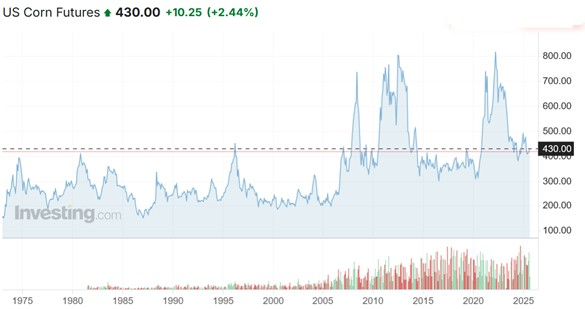
\includegraphics[width=0.5\textwidth]{figures/corn.jpg}
\end{center}

Mexico is structurally short yellow corn and imports most of it from the U.S., while white corn is central for tortillas. Policy has been in flux: Mexico's 2023 decree targeted biotech corn for human consumption and instructed a gradual substitution in other uses, triggering a USMCA dispute \citep{fas_mexico_decree_2023,ustr_usmca_biotech_2023}. In December 2024 the US prevailed at the USMCA panel \citep{ustr_usmca_biotech_win_2024}; Mexico has kept a domestic planting ban while adjusting import measures \citep{reuters_mexico_gm_ban_2025,fas_mexico_grain_annual_2025}. These shifts, together with U.S. supply and logistics, transmit into Mexican basis, feed costs, and tortilla inflation dynamics.

ZCZ5 denotes the CBOT Corn futures contract for December 2025 delivery (month code Z). Each contract is 5{,}000 bushels; tick size is $1/4$ cent per bushel (\$12.50 per contract) \citep{barchart_zc_specs}.
Recent U.S. balance-sheet news also matters: USDA has projected very large 2025 U.S. corn production, which weighs on deferred contracts like ZCZ5, all else equal \citep{reuters_record_crop_2025}.
% (Optional) Add a footnote if you want month codes spelled out.
\footnote{CBOT month codes: H=Mar, K=May, N=Jul, U=Sep, Z=Dec \citep{barchart_zc_specs}.}

\subsection{Interpretation of \texorpdfstring{ZCZ25}{ZCZ25} (one-day read)}

\begin{center}
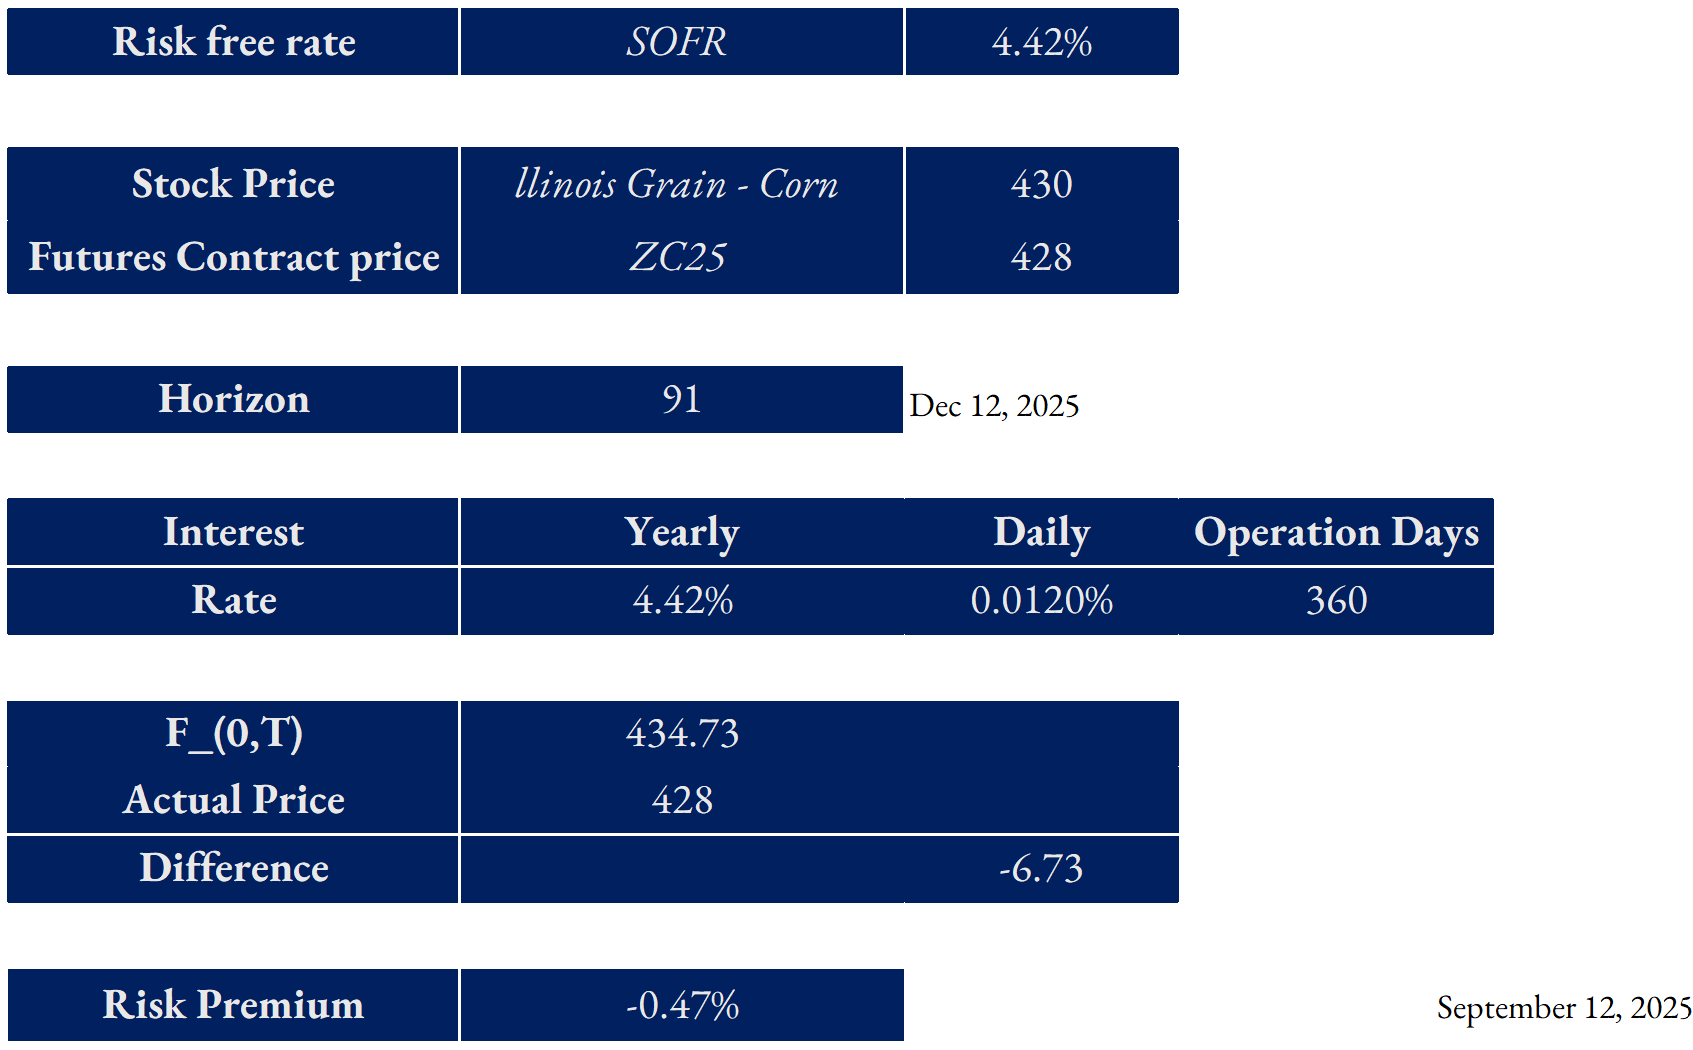
\includegraphics[width=0.5\textwidth]{figures/corn2.png}
\end{center}

A 91-day horizon (ACT/360) is used with $S=430.00$ ¢/bu for Illinois cash corn, $F=428.00$ ¢/bu for \textbf{ZCZ5}, and $r=4.41\%$. The no-carry fair value is obtained from $F^{\*}=S\,e^{rT}$, yielding
\[
T=\tfrac{91}{360},\quad F^{\*}=430\,e^{0.0441\cdot T}\approx \mathbf{434.72}\ \text{¢/bu}.
\]

A price difference of $\mathbf{-6.72}$ ¢/bu is observed $(F-F^{\*})$, which equals \textbf{26.9 ticks} and \textbf{\$336 per 5,000-bu contract}. The spot–futures return $F/S-1$ is $\mathbf{-0.47\%}$.

For interpretation, the cost-of-carry relation
\[
F=S\,e^{(r+u-y)T}
\]
is used, where $u$ represents storage and insurance costs and $y$ the convenience (or inventory) yield. The market carry is inferred as
\[
c_{\text{mkt}}=\frac{1}{T}\ln\!\frac{F}{S}
=\frac{1}{91/360}\ln\!\frac{428}{430}\approx \mathbf{-1.84\%}\ \text{per year}.
\]

It follows that the net convenience yield is obtained as
\[
y-u \approx r-c_{\text{mkt}}\approx 4.41\%-(-1.84\%)=\mathbf{6.25\%}\ \text{per year}.
\]

Therefore, a \textbf{negative basis} and $F<S e^{rT}$ are consistent with \textbf{backwardation}: near-dated corn is priced below pure financing carry because inventory availability, storage constraints, or location basis premia raise the value of holding physical grain now. The deviation is explained by $y$ and operational frictions, so it is interpreted as an inventory/logistics signal rather than a tradable arbitrage.

\subsection{Futures terms structure (12 Sep 2025)}

\paragraph{Rule of thumb:} Corn quotes are \textbf{cents per bushel}. Format \texttt{430'0} = \textbf{430.00 ¢/bu}. Tick \texttt{'2} = \textbf{0.25 ¢} = \textbf{\$12.50} per 5,000-bu contract. \textbf{1 ¢ = \$50}.

\subsubsection*{Curve and carries}

\begin{itemize}
  \item \textbf{Up to Jul-26:} rising settles $\Rightarrow$ \textbf{contango}.
    \begin{itemize}
      \item Z25 430'0 $\rightarrow$ H26 447'2: spread \textbf{+17'2 = 17.25 ¢}. Roughly 3 months $\Rightarrow$ carry $\approx 17.25/430 \approx 4.0\%$ over the period, \textbf{$\sim$16\% annualized}.
      \item H26$\rightarrow$K26: \textbf{+9'6 = 9.75 ¢}.
      \item K26$\rightarrow$N26: \textbf{+6'4 = 6.50 ¢}.
    \end{itemize}
  \item \textbf{Harvest kink:} N26 463'4 $\rightarrow$ U26 459'6 = $-3'6 = -3.75$ ¢. New-crop discount at harvest.
  \item \textbf{Back to carry:} U26 459'6 $\rightarrow$ Z26 469'0 = $+9'4 = 9.50$ ¢.
  \item \textbf{Far strip:} classic pattern repeats. N27 492'0 $\rightarrow$ U27 470'6 = $-21'4$ big harvest discount, then U27$\rightarrow$Z27 $+2'6$.
\end{itemize}

\textbf{Interpretation:} Ample old-crop stocks and positive financing/storage net of convenience yield pre-harvest. \textbf{Harvest months invert} on expected supply surge, then carries re-emerge as grain moves into storage.


\subsection{Weekly term-structure diagnostics (5–12 Sep 2025)}

\subsubsection*{Daily move}

Parallel bull. \textbf{Z25 +10'2 = +10.25 ¢ ($\sim$+2.4\%)}, H26 +10'0, tails +6'2 to +9'0. Shape largely intact. Rally is spot-led rather than curve-shape driven.

\subsubsection*{Liquidity}

Heavy near-dated flow. \textbf{Z25 vol 343k, OI 852k.} H26 111k vol. Back months thin and mostly marks. Use Z-H-K-N for execution and for clean curve reads.

\subsubsection*{Carry economics}

Cost-of-carry model $F=S\,e^{(r+u-y)T}$. Contango says $r+u>y$. Inversions at \textbf{U} reflect higher convenience yield around harvest or anticipated large new-crop availability. If rates fall or stocks tighten, carries \textbf{compress}; harvest inversions \textbf{shrink} or flip.

\subsubsection*{Tactics}

\begin{itemize}
  \item \textbf{Directional bull:} prefer \textbf{near months} for higher spot beta. Hedge roll with a \textbf{flattener} if you expect stocks to tighten.
  \item \textbf{Carry view:}
    \begin{itemize}
      \item Expect \textbf{more carry} $\rightarrow$ position for \textbf{steepeners} (near cheaper vs far).
      \item Expect \textbf{tightness} $\rightarrow$ \textbf{flatteners} (long near, short far) benefit if Z-H narrows from +17'2.
    \end{itemize}
  \item \textbf{Hedgers:}
    \begin{itemize}
      \item \textbf{Producers} forward-sell deferred to lock today’s rich carries.
      \item \textbf{Users} favor near coverage and layer into harvest dips.
    \end{itemize}
\end{itemize}

\subsubsection*{Quick conversions}

\begin{itemize}
  \item \textbf{Z25 settle 430'0 = \$4.300/bu.}
  \item \textbf{Z25--H26 +17'2} = \textbf{\$0.1725/bu} carry $\approx$ \textbf{\$862.50/contract} over the quarter.
\end{itemize}

\section{Crude Oil}

\subsection{Recent developments}
Crude oil remains anchored by the classical triad of fundamentals, policy coordination, and dollar conditions. Global demand growth and inventory paths continue to govern the balance; OPEC+ supply management modulates prompt availability; and the USD transmits monetary conditions into non-USD purchasing power \citep{eia_prices_2023,eia_opec_2024,bis_usd_commodity_2023,ecb_oil_usd_2024}. Into mid-September 2025, front-WTI traded in the low \$60s per barrel while carry signals pointed to persistent, though not extreme, prompt tightness.

\subsection{Spot \& futures}
WTI spot reflects contemporaneous physical scarcity and the USD level; by contrast, the futures curve prices the intertemporal trade-off between holding inventory and deferring delivery. The standard cost-of-carry relation is used:
\[
F_T=S_0\,e^{(r+u-y)T},
\]
with \(r\) the USD funding rate, \(u\) storage/insurance, and \(y\) the convenience (lease) yield. Backwardation (\(F_T<S_0e^{rT}\)) occurs when \(y>r+u\); contango when \(y<r+u\). Contract units and expiries follow CME specifications for WTI (1{,}000 bbl, USD/bbl) \citep{cme_cl_specs,cme_cl_calendar}. Risk-neutral “no-carry” fair values in this report use \(F^{*}=S_0 e^{rT}\) with SOFR-based \(r\) \citep{frbny_sofr}.

\subsection{Mexico-linked implications}
For Mexico, oil levels and curve shape transmit through fiscal and external accounts. Higher spot improves upstream realized prices and state revenues; pronounced backwardation raises the value of prompt barrels relative to deferrals, but compresses the forward cover available to hedge future cash flows. Conversely, contango lowers prompt realizations but cheapens deferred hedges. Given Pemex’s financing and investment plans, a stable, shallow backwardation is operationally preferable to extreme tightness: it supports near-term cash margins while avoiding destabilizing roll dynamics \citep{reuters_oil_peak_2008,worldbank_oil_spike_2008}. Policy levers that reduce logistics and storage frictions effectively lower \(u\) and stabilize basis, improving the translation from global prices to domestic income.

\paragraph{Transmission channels.}
Three first-order channels transmit crude dynamics into Mexico’s macro-financial stance: (i) the \emph{fiscal} channel via upstream realized prices, production volumes \(Q_t\), and the Maya/WTI differential; (ii) the \emph{external} channel through the hydrocarbon trade balance (crude exports vs.\ refined-product imports); and (iii) the \emph{financial} channel via USD/MXN, sovereign risk premia, and the equity cost of capital for energy-linked corporates. Formally, upstream cash margin is \(M_t \approx Q_t\,[S_t-\delta_t]-\text{OPEX}_t\), where \(S_t\) is the benchmark (WTI/Brent proxy), \(\delta_t\) the quality/location discount (e.g., Maya to WTI), and \(\text{OPEX}_t\) operating costs. Fiscal intake and external balances scale with \(M_t\) and with the sign of refined-product net imports.

\paragraph{Role of curve shape for cash-flow timing.}
With \emph{orderly backwardation} and modest day-to-day parallel level moves, prompt barrels are valued above deferred. This configuration is advantageous for near-term monetization but reduces the forward price available for long-dated hedges. In accounting terms, a government or SOE hedger that sells \(n\) futures across a ladder \(\{T_i\}\) locks
\[
\mathbb{E}[\text{Revenue}] \approx \sum_i Q_{T_i}\,F_{T_i},
\]
so backwardation (\(F_{T_i}<S_0 e^{rT_i}\)) lowers hedge strikes even as it supplies \emph{positive roll} to long consumers. Conversely, contango would raise forward strikes but erode consumer roll. The week’s diagnostics show stable \(y-u\) at short horizons; hedge design can therefore prioritize \emph{tenor diversification} rather than chasing transient slope noise.

\paragraph{Logistics, storage, and basis.}
Domestic logistics and storage conditions map into the effective \(u\) and into location basis \(\delta_t\). Lower pipeline/terminal frictions reduce \(u\) and compress \(\delta_t\), improving pass-through from global benchmarks to domestic realizations. In backwardation, low working inventories are rational; however, excessively lean stocks amplify downside tail risk if \emph{y} spikes. A policy mix that keeps minimum operational inventories while upgrading storage flexibility reduces the volatility of \(M_t\) without materially sacrificing carry.

\paragraph{FX and monetary-policy interactions.}
Higher crude supports the terms of trade and, conditional on global risk, can be MXN-supportive. Yet FX pass-through to domestic fuel prices affects headline inflation. If policy opts for partial smoothing (implicit fuel-price stabilization), fiscal buffers must be pre-committed or hedged. Otherwise, inflation volatility tightens the constraint set for monetary policy. Practically, energy-linked issuers should pair oil hedges with FX overlays to stabilize MXN cash flows; otherwise, USD price gains can be offset by MXN appreciation.

\paragraph{Corporate treasury and investor implementation.}
For upstream exposure, a \emph{laddered short} in the liquid front two or three contracts balances execution depth and slope risk; the documented stability of short-dated \(y-u\) argues for systematic rebalancing rather than discretionary timing. For refiners/marketers, \emph{long prompt / short deferred} structures monetize positive roll in backwardation while capping input-cost spikes. Cross-asset investors can express macro views via \emph{curve trades}: expected inventory rebuilds or lower USD rates support flatteners (long near/short far); persistent OPEC+ discipline or logistics constraints support steepeners in backwardation.

\paragraph{Policy and operating priorities.}
(i) \emph{Lower \(u\)}: invest in storage reliability and throughput to reduce effective storage/operational costs and to smooth basis.  
(ii) \emph{Standardize hedging governance}: publish a clear tenor ladder and risk limits; disclose hedge strikes and coverage ratios to anchor funding costs.  
(iii) \emph{Integrate FX and commodity risk}: mandate MXN cash-flow stabilization targets with coordinated oil–FX overlays.  
(iv) \emph{Transparency on quality differentials}: regular disclosure of the Maya/WTI (or delivered) differential \(\delta_t\) improves revenue forecasting and reduces uncertainty premia.

\paragraph{Net assessment.}
Given spot in the low \$60s and shallow, stable backwardation, near-term upstream margins are supported while roll dynamics remain manageable. The configuration benefits Mexico if logistics keep \(u\) contained and if hedging policy converts favorable prompt economics into stable, multi-quarter MXN cash flows. The principal risks are a shock to inventories (deepening backwardation and basis) or a USD-driven tightening in global financial conditions; both warrant pre-defined hedge and liquidity triggers.


\subsection{Futures term structure (12 Sep 2025)}
\textbf{Shape and slopes.} The strip exhibits \emph{orderly backwardation}:
\[
\text{Oct-25 } \mathbf{62.69} \;\rightarrow\; \text{Dec-25 } \mathbf{62.19}
\;\rightarrow\; \text{Mar-26 } \mathbf{61.95}
\;\rightarrow\; \text{Dec-26 } \mathbf{61.77}
\;\rightarrow\; \text{Oct-27 } \mathbf{62.08}.
\]
The 1-year slope (Oct-25\(\to\)Oct-26) is \(61.74/62.69-1\approx \mathbf{-1.52\%}\) p.a., implying \(r+u-y\approx -1.5\%\) p.a. (therefore \(y>r+u\)). A slight re-steepening at the very back is consistent with normalization of tightness beyond one year.

\textbf{Daily move.} A near-parallel \(\,+0.32\) to \(+0.36\) USD/bbl shift is observed across the strip on the session, read as a \emph{spot-led} rally with curve shape broadly preserved—i.e., news raised the level, not the intertemporal premium.

\textbf{Carry and rolls.} Calendar spreads such as Oct/Nov \(+0.27\), Nov/Dec \(+0.23\), and Oct/Dec \(+0.50\) encode positive roll income for long-only consumers and negative roll for producer shorts in the current backwardation regime.

\subsection{Interpretation of \texorpdfstring{CLV25}{CLV25} (one-day read)}
Using \(S_0=\$62.69\), \(r=4.41\%\) (ACT/360), and \(T=10/360\), the no-carry fair is
\[
F^{*}=S_0 e^{rT} \approx 62.69\,e^{0.0441\cdot(10/360)}=\mathbf{62.765}.
\]
The observed settlement \(F=\mathbf{62.69}\) implies \(F<F^{*}\) by \(\$0.075\) (backwardation). Two equivalent diagnostics are used:

\(\bullet\) \emph{Market carry vs.\ spot:} \(c_{\text{mkt}}=\frac{1}{T}\ln(F/S_0)\approx 0\) p.a., since \(F\approx S_0\).

\(\bullet\) \emph{Net convenience minus storage:} from \(F/F^{*}=e^{(u-y)T}\),
\[
y-u=\frac{1}{T}\ln\!\Big(\frac{F^{*}}{F}\Big)\approx \mathbf{4.32\%}\ \text{p.a.}
\]
Numerically, \(y-u\) is close to \(r\), indicating that the discount to \(F^{*}\) is largely explained by convenience yield offsetting financing (with storage \(u\) small at the 10-day horizon). This is the canonical signature of \emph{mild but persistent prompt tightness} \citep{eia_backwardation_2013,milonas_convenience_2024}.

\subsection{Weekly term-structure diagnostics (5–12 Sep 2025)}
\textbf{Data.} SOFR ranged \(4.39\)–\(4.42\%\); horizons declined from 17 to 10 days. Spot and front futures were essentially equal each day; the theoretical no-carry fair \(F^{*}\) exceeded market by \(\$0.075\)–\(\$0.127\).

\textbf{Finding 1: stable backwardation intensity.} Although \((F-F^{*})\) becomes less negative through the week, this is \emph{mechanical time decay}—as \(T\downarrow\), the present-value gap from financing shrinks. The carry metric that nets out horizon effects,
\[
y-u=\frac{1}{T}\ln\!\Big(\frac{F^{*}}{F}\Big),
\]
is remarkably stable at \(\mathbf{4.30\%{-}4.33\%}\) p.a. each day. Hence, the convenience yield continues to offset funding with little drift.

\textbf{Finding 2: spot-led level variation, curve preserved.} Day-to-day price changes are dominated by spot (macro/USD) rather than by shifts in \((r+u-y)\). This matches the session commentary above: level up-moves occur with an approximately unchanged slope, consistent with fundamentals/news raising the spot anchor while physical tightness stays moderate \citep{eia_prices_2023,eia_opec_2024,bis_usd_commodity_2023}.

\textbf{Finding 3: micro implications.} For longs, backwardation provides positive roll yield into expiry; for producer shorts, rolls are a headwind but hedge effectiveness is high because \(y-u\) is stable. The absence of sharp slope changes reduces basis risk for short-dated hedges.

\subsection{Does this benefit Mexico? What should be done}
\textbf{Benefit.} The configuration—spot in the low \$60s with steady, shallow backwardation—supports upstream cash flow and state revenue without imposing extreme roll costs or volatility.

\textbf{Investor actions (policy-neutral).}
\begin{enumerate}
  \item \emph{Decompose risks.} Manage level risk (spot) and term risk (roll/carry) separately. Use short-dated futures for beta; use calendar spreads to express views on slope normalization.
  \item \emph{Hedge structure.} Producer hedges can be laddered in the front two contracts to exploit stable backwardation; consumers can pre-buy prompt barrels and keep deferred cover lighter to benefit from positive roll.
  \item \emph{Trigger mapping.} Monitor OPEC+ guidance and U.S. rate moves: a durable fall in \(r\) or inventory builds should flatten the curve; tightening logistics raises \(y\) and deepens backwardation.
\end{enumerate}

\textbf{Policy/operating recommendations for Mexico.}
\begin{enumerate}
  \item \emph{Lower logistics/storage frictions.} Reducing \(u\) via infrastructure and operational reliability improves realized margins and stabilizes basis.
  \item \emph{Hedge governance.} Standardize hedge programs that couple oil price hedges with FX overlays to dampen peso-revenue volatility.
  \item \emph{Transparency and cadence.} Publish regular hedge/carry metrics (e.g., inferred \(y-u\)) alongside production guidance to anchor market expectations and lower funding costs.
\end{enumerate}



\section{Crude Oil}
Crude oil is one of the most important energy commodities, powering transportation, industry, and heating. Therefore, its price is influenced by a complex array of factors. One of the most significant is the balance between global supply and demand. During periods of strong economic growth, demand for oil increases due to higher transportation and manufacturing activity. Conversely, economic recessions can lead to a sharp drop in demand and lower prices \citep{eia_prices_2023}.

The decisions made by the Organization of the Petroleum Exporting Countries (OPEC) and its allies (OPEC+) are also a primary influence on oil prices. This group coordinates production levels among major oil-exporting nations. By restricting or increasing output, they can directly tighten or loosen global supply to stabilize or manipulate the market \citep{eia_opec_2024}.

Geopolitical events are a major source of price volatility. Conflicts, sanctions, or political instability in key oil-producing regions (like the Middle East, Russia, or Venezuela) can disrupt supply chains and threaten actual production, leading to fears of a shortage and spiking prices \citep{eia_prices_2023}.

Furthermore, fluctuations in the U.S. dollar significantly affect oil prices. Since oil is globally traded in U.S. dollars, a stronger dollar makes oil more expensive for countries using other currencies, which can dampen demand. A weaker dollar makes oil cheaper on international markets, potentially boosting demand \citep{bis_usd_commodity_2023,ecb_oil_usd_2024}.

In 2008, crude oil prices reached a historic peak. That July, the price of West Texas Intermediate (WTI) crude oil futures hit an all-time nominal high of \$147.27 per barrel. This surge was driven by a combination of robust global demand, geopolitical tensions, and significant financial speculation. From the start of 2007 to this peak, the price had increased by over 200\%. The subsequent crash later that year, as the global financial crisis crushed demand, demonstrates the extreme volatility of the oil market \citep{reuters_oil_peak_2008,worldbank_oil_spike_2008}.

\textbf{CLV25} refers to the WTI (West Texas Intermediate) crude oil futures contract that expires in October 2025. Each contract represents 1{,}000 barrels and is quoted in U.S. dollars (USD) per barrel \citep{cme_cl_specs,cme_cl_calendar}.
This table compares the spot price, \$62.69, with what the futures price “should” be over 10 days using the 4.41\% annual risk-free rate and assuming there are no extra costs/benefits such as dividends \citep{frbny_sofr}.


\subsection{Interpretation of \texorpdfstring{CLV25}{CLV25} (one-day read)}
\begin{center}
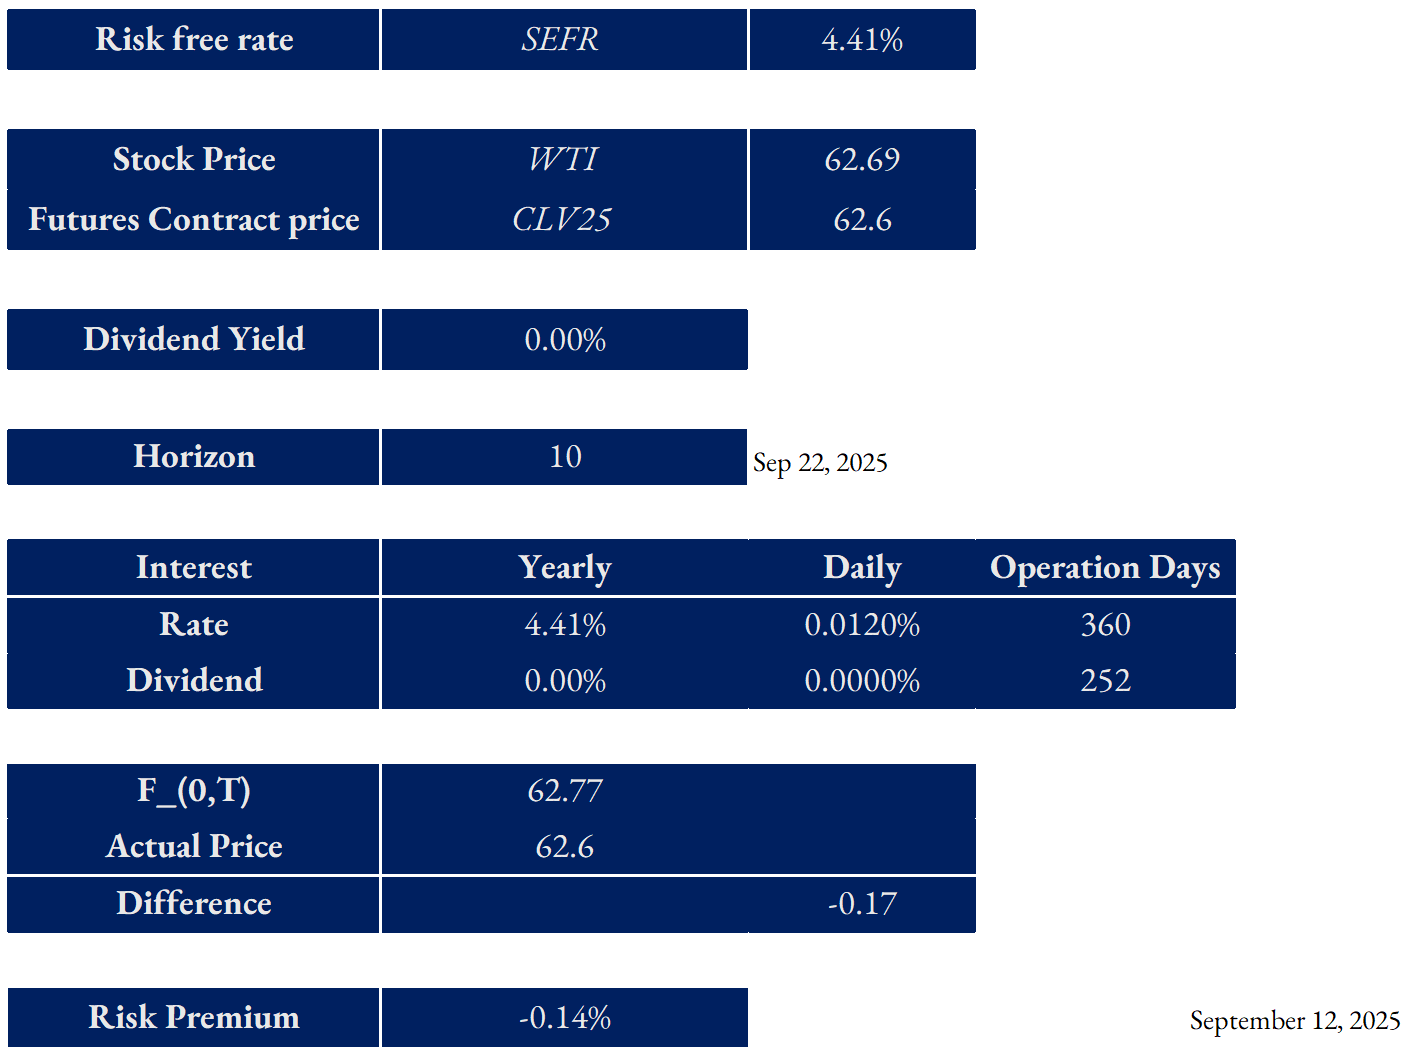
\includegraphics[width=0.5\textwidth]{figures/wti.png}
\end{center}

With those inputs, the theoretical price is computed as $F_{0,T} \approx S_0(1 + rT)$. For 10 days, $rT \approx 0.0441 \times \frac{10}{360} = 0.1225\%$. Therefore, $F_{0,T} \approx 62.69 \times (1 + 0.001225) = 62.77$. The market, however, is at 62.60. That means the actual futures price is \$0.17 per barrel below the theoretical value.

In percentage terms, the “risk premium” shown in the table is $-0.14\%$. That comes from comparing the futures price to spot: $62.60/62.69 - 1 \approx -0.14\%$. By contrast, the $-\$0.17$ difference you highlight is the gap between the market futures price and the theoretical futures price.

Economically, this discount indicates mild backwardation: the nearby contract is worth slightly less than what the interest rate alone would imply. In commodities like crude oil, this is often interpreted as an implicit convenience yield (the benefit of holding the physical now) that offsets the interest rate \citep{kaldor_working_brennan, eia_backwardation_2013, milonas_convenience_2024}. Roughly, the total deviation from the theoretical value is $\sim 0.2625\%$ over 10 days, which annualizes to about a $9.5\%$ convenience yield net of costs.

Practically speaking, for the standard contract size (1{,}000 barrels), that \$0.17 amounts to \$170 per contract \citep{cme_cl_specs}.


A 10-day valuation window is used with $S=62.69$, $F=62.60$, and $r=4.41\%$ (ACT/360). The no-carry fair value is computed as
\[
F^{\*}=S\,e^{rT}=62.69\,e^{0.0441\cdot(10/360)}\approx62.77.
\]

A price difference of
\[
-\$0.17
\]
per barrel is observed $(F-F^{\*})$, which corresponds to 17 ticks (\$170 per standard 1,000-barrel contract). In percentage terms, a spot–futures discount of
\[
\frac{F}{S}-1 \approx -0.14\%
\]
is obtained.

For interpretation, the cost-of-carry relation
\[
F=S\,e^{(r+u-y)T}
\]
is used, where $u$ denotes storage/insurance costs and $y$ denotes the convenience yield. The market carry is inferred as
\[
c_{\text{mkt}}=\frac{1}{T}\ln\!\frac{F}{S}\approx-5.17\%\ \text{per year},
\]
and the net convenience yield is obtained as
\[
y-u \approx r-c_{\text{mkt}}\approx 4.41\%-(-5.17\%)=9.6\% \ \text{per year}.
\]

Hence, the observed discount is consistent with \textbf{backwardation}: inventory is valued sufficiently highly (or storage is constrained) so that $y$ more than offsets financing $r$ and any $u$. No-arbitrage is preserved because $y$ and operational frictions are not directly tradable; the deviation is therefore read as a signal of tight near-term balances rather than a free arbitrage.

\subsection{Weekly term-structure diagnostics (5–12 Sep 2025)}


\subsection{Futures terms structure (12 Sep 2025)}
\paragraph{Backwardation.} Front $>$ deferred. Positive convenience yield.

\subsubsection*{Curve and slope}
\begin{itemize}
  \item Settles: \textbf{Oct-25 62.69 $\rightarrow$ Dec-25 62.19 $\rightarrow$ Mar-26 61.95 $\rightarrow$ Dec-26 61.77 $\rightarrow$ Oct-27 62.08}.
  \item 1-yr slope (Oct-25$\rightarrow$Oct-26): $61.74/62.69-1\approx -1.52\%$ $\Rightarrow$ $(r+u-y)\approx -1.5\%$ p.a. $\Rightarrow$ $y>r+u$.
  \item Back end re-steepens slightly into Oct-27.
\end{itemize}

\subsubsection*{Session move}
\begin{itemize}
  \item Near-parallel \textbf{+0.32 to +0.36 \$/bbl} across the strip. Spot-led rally, curve shape broadly unchanged.
\end{itemize}

\subsubsection*{Liquidity/microstructure}
\begin{itemize}
  \item Heavy flow front: \textbf{Oct-25 vol 313k, OI 157k}; \textbf{Nov-25 188k/260k}, \textbf{Dec-25 145k/280k}. Backs thinner; many \textbf{A/B} are quotes, not prints. Total \textbf{vol 913k, OI 1.95M}.
\end{itemize}

\subsubsection*{Calendar spreads (carry)}
\begin{itemize}
  \item \textbf{Oct/Nov +0.27}, \textbf{Nov/Dec +0.23}, \textbf{Oct/Dec +0.50} (front richer).
  \item Long-only roll is \textbf{positive} in backwardation: sell high near, buy lower deferred. Short roll is negative.
\end{itemize}

\subsubsection*{Economic read}
\begin{itemize}
  \item Backwardation signals \textbf{tight prompt balances} or expected \textbf{inventory draws}.
  \item If USD rates fall or inventories build, curve should \textbf{flatten} (less backwardation).
  \item Shape is cost-of-carry: $F=S\,e^{(r+u-y)T}$. Here $y$ dominates.
\end{itemize}

\subsubsection*{Tactics}
\begin{itemize}
  \item Directional bull: prefer near months for higher beta; hedge roll with \textbf{long near / short far} if you expect flattening.
  \item Producers: hedge in deferred where backwardation lowers forward price but roll works against shorts.
  \item Consumers: near-dated longs benefit from roll; layer hedges if you fear prompt spikes.
\end{itemize}

\subsubsection*{Next diagnostics (if you have spot $S$)}
Estimate convenience yield:
\[
y \approx r+u-\frac{1}{T}\ln\left(\frac{F_T}{S}\right),
\]
by month to see where tightness concentrates.










\section{Silver}

\subsection{Economic role and macro-financial channels}
Silver is a dual-use metal with a large industrial footprint (electronics, photovoltaics, medical and chemical applications) and a non-trivial investment component. As a result, its pricing is shaped by both end-use demand and financial conditions. Cyclical expansions raise manufacturing throughput and technology adoption, lifting physical offtake; global slowdowns reverse that impulse. Monetary policy and term premia transmit through discount rates and the USD: a stronger dollar tightens global financial conditions and lowers non-USD purchasing power, dampening demand for dollar-priced commodities; a softer USD does the opposite \citep{silver_institute_wss_2024,usgs_silver_mcs_2024,bis_usd_commodity_2023}.

\begin{figure}[h]
\centering
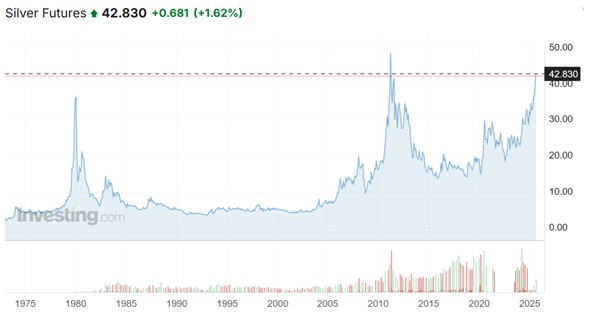
\includegraphics[width=0.7\textwidth]{figures/silver_time_series.jpg}
\caption{COMEX silver futures time series (illustrative). Source: Investing.com.}
\label{fig:silver_time_series}
\end{figure}

\subsection{Policy and geopolitical drivers}
Trade restrictions, tariffs, sanctions, and logistics frictions reallocate flows across refining hubs and end-user markets, altering local basis and inventory dynamics; these mechanisms operate alongside the macro channels above \citep{silver_institute_wss_2024}.

\subsection{Historical stress episode}
The 1980 episode (“Silver Thursday”) illustrates how leverage, concentrated positioning, and margining can dominate price discovery. After a speculative run-up to \$49.45/oz, rule changes and margin calls precipitated a sharp decline on March 27, 1980, with broader market spillovers \citep{britannica_silver_thursday,nyt_1980_silver_thursday}.

\subsection{Recent developments}
In early September 2025, spot silver traded above \$40/oz and marked 14-year highs amid rising Fed-easing probabilities and a weaker USD; research commentary highlighted ETF inflows and a persistent physical deficit \citep{reuters_silver_14y_sep1,reuters_tradingday_sep11,reuters_anz_raises_silver,lbma_q2_2025}. Corporate activity remains supportive for Mexico-centric supply, including consolidation around the Juanicipio asset \citep{reuters_paasmag}. Spot benchmarking relies on the LBMA Silver Price, while COMEX futures provide standardized exposure and hedging along the term structure \citep{lbma_prices,cme_silver_overview}.

\paragraph{Mexico: why it matters.}
Mexico is the world’s largest silver producer, so revenue, royalties, and FX inflows are sensitive to the level and volatility of silver. Higher prices improve internal cash generation and capex flexibility; conversely, regulatory or logistical frictions widen local basis and delay monetization. Through the terms-of-trade channel, stronger silver can be peso-supportive when broader macro conditions are aligned \citep{reuters_mx_top_silver}.

\subsection{Spot \& futures}
The spot price refers to unallocated silver in London (or a deliverable loco) and is used to value immediate transactions and inventories. COMEX futures internalize financing and inventory economics over horizon \(T\) via the cost-of-carry relation
\[
F=S\,e^{(r+u-l)T},
\]
with \(r\) the USD funding rate, \(u\) storage/insurance, and \(l\) the lease (convenience) rate. Tight nearby physical conditions raise \(l\) and can generate backwardation \((F<S\,e^{rT})\); abundant storage and higher financing tilt the curve toward contango. Thus, spot primarily reflects contemporaneous scarcity and dollar conditions, while futures reflect the intertemporal trade-off between owning inventory today versus financing delivery later.

The \emph{spot} benchmark is the LBMA Silver Price (or XAG/USD quotes for unallocated metal in London); it is used to value immediate physical transactions, inventory revaluation, and cash-market settlements \citep{lbma_prices}. The COMEX futures curve is used to transfer price risk across time and to standardize hedging and speculative exposure; contract design, margining, and delivery mechanics shape its microstructure \citep{cme_silver_overview}. In practice, three news-sensitive wedges separate spot from futures: (i) the \emph{financing–storage–lease} term in the cost-of-carry \(F=S\,e^{(r+u-l)T}\), (ii) \emph{location/quality} basis between London unallocated and COMEX-deliverable bars, and (iii) \emph{timing} basis linked to near-term ETF creations/redemptions and refinery/warehouse flows. When easing U.S. rate expectations strengthen non-USD demand and ETF creations accelerate, it is common that spot tightens faster than the curve (lease rate \(l\uparrow\)), generating transient backwardation; as inventories are replenished and funding/storage regain prominence, slight contango reappears. Hence, spot is used as a barometer of contemporaneous scarcity and USD conditions, whereas futures are used to price the intertemporal trade-off between carrying inventory and deferring settlement.

\subsection{Mexico-linked implications}
Near-term shipments monetize elevated spot first; medium-dated cash flows depend on the curve’s carry and roll costs. Hedge design should distinguish (i) price level risk (spot) from (ii) term-structure risk (roll yield and basis), recognizing that cross-currency and policy shocks can modulate both even when the global price is strong.

Mexico’s role as the world’s largest silver producer means that domestic cash flows, royalties, and FX receipts are highly exposed to these spot–futures dynamics \citep{reuters_mx_top_silver}. The following news-driven scenarios are operationally relevant:
\begin{enumerate}
  \item \textbf{ETF inflow surges and USD weakness.} Spot premia rise first; it is used by producers with near-term shipments to monetize higher LBMA realizations. If COMEX contango persists, rolling short futures hedges entails modest carry costs; if backwardation appears, rolls can be revenue-positive.
  \item \textbf{Refinery or logistics bottlenecks.} Delays in moving Mexico-origin doré or concentrates to refiners widen the location basis versus London. It is used to hedge with COMEX futures, but performance depends on the basis path; treasury policy should stress-test basis risk alongside price risk.
  \item \textbf{Funding-cost swings.} Shifts in dollar funding alter \(r\) and, with stable lease \(l\), move the curve even if spot is unchanged; this is used to reassess hedge tenors because forward premia/discounts change while realized sales prices do not.
  \item \textbf{Domestic policy shocks.} Changes in royalties, permitting, power tariffs, or labor conditions affect mining margins and supply timing; it is used to adjust production hedges and to reassess the mix of spot sales versus forward coverage given altered cash-need profiles.
  \item \textbf{FX interaction (USD/MXN).} Stronger silver improves Mexico’s terms of trade and can support MXN conditionally on global risk; however, a stronger MXN reduces peso revenues for unhedged USD sales. It is used to pair metal hedges with FX hedges to stabilize MXN cash flows.
\end{enumerate}
In summary, elevated spot levels benefit near-term Mexican exports directly, while the sign and size of the futures basis determine carry and roll outcomes on hedges. Policy- and logistics-sensitive basis risk is material; it is used to complement price hedging with explicit basis and FX risk management, recognizing that the curve reflects financing and inventory conditions that need not move one-for-one with spot.



\subsection{Futures term structure (12 Sep 2025, integrated read)}

\paragraph{Framework.}
The silver curve on \emph{12 Sep 2025} is interpreted through the cost-of-carry relation
\[
F_T = S_0\,e^{(r+u-l)T},
\]
where \(r\) is USD funding, \(u\) storage/insurance, and \(l\) the lease (convenience) rate. Curve \emph{shape} identifies the sign and size of \((r+u-l)\); parallel \emph{level} moves are used to diagnose spot-led shocks, while \emph{non-parallel} moves are used to diagnose changes in carry/inventory conditions.

\paragraph{Curve shape and levels.}
A clear \emph{contango} is observed across listed maturities:
\[
\text{SEP-25 } \mathbf{42.387}\ \rightarrow\ \text{DEC-25 } \mathbf{42.830}\ \rightarrow\ \text{MAR-26 } \mathbf{43.322}\ \rightarrow\ \text{DEC-26 } \mathbf{44.682}\ \rightarrow\ \text{MAR-27 } \mathbf{45.089}\ \rightarrow\ \text{SEP-27 } \mathbf{45.877}.
\]
The one-year slope (DEC-25 \(\rightarrow\) DEC-26) is
\[
\frac{44.682}{42.830}-1 \approx \mathbf{4.32\%}\ \text{p.a.},
\]
and the two-year slope (SEP-25 \(\rightarrow\) SEP-27) is
\[
\Big(\frac{45.877}{42.387}\Big)^{1/2}-1 \approx \mathbf{4.04\%}\ \text{p.a.}
\]
These slopes are used as reduced-form estimates of \((r+u-l)\) over the corresponding horizons, implying \(r+u-l\gtrsim 4\%\) p.a.; inventories are not tight enough to invert the curve (\(l\) does not dominate \(r+u\)).

\paragraph{Daily move and decomposition.}
A near-parallel increase of about \(\mathbf{+0.68}\) USD/oz along the strip (\(\sim \mathbf{+1.6\%}\) at the front) is observed. Parallelism is used to attribute the move primarily to a \emph{spot-led shock} (e.g., dollar softness and investor demand), while the persistence of contango indicates that intertemporal premia \((r+u-l)\) are broadly unchanged on the day. This diagnosis is consistent with the one-day SIZ25 read, where slight contango is obtained despite elevated spot.

\paragraph{Liquidity and microstructure.}
Open interest and volume concentrate in \textbf{DEC-25} (vol \(\approx 72{,}263\), OI \(\approx 133{,}690\)); \textbf{MAR-26} is the secondary node (vol \(\approx 2{,}265\), OI \(\approx 16{,}343\)). It is used to execute hedges and curve views primarily in these nodes to minimize execution and basis risk. Quotes in thin months are often marking references rather than active trading venues.

\paragraph{Carry and roll math.}
Calendar spreads summarize carry costs and roll P\&L:
\[
\text{DEC-25/MAR-26} \approx +0.492,\qquad \text{DEC-25/DEC-26} \approx +1.852.
\]
In contango, long futures positions face \emph{negative roll yield} if spot is unchanged (convergence down toward spot); short positions benefit from carry. This mapping is used in hedge design (e.g., producer shorts) and in curve trades (e.g., flatteners/steepeners).

\paragraph{Macro levers mapped to shape.}
Three levers are used to connect macro news to curve diagnostics: (i) \emph{rates}—lower USD rates compress \((r+u-l)\) and flatten contango; (ii) \emph{inventory/lease}—tight physical markets raise \(l\), flattening or inverting the curve; (iii) \emph{storage/operations}—changes in storage and insurance costs shift \(u\), steepening or flattening depending on direction. The observed contango with a parallel up-move is, therefore, read as “risk-on/spot-led, inventory not binding.”

\paragraph{Implementation tactics.}
Directional bulls are typically routed to near maturities for higher spot beta and may hedge roll via calendar spreads (e.g., long DEC-25 / short MAR-26) if carry is expected to compress. Industrial users hedging inputs are advised to lock deferred maturities knowingly that the quoted contango is the carrying cost they pay. Curve views are implemented as \emph{flatteners} if easing USD rates or tighter inventories are expected; otherwise, \emph{steepeners} are preferred.

\paragraph{Diagnostics for inference.}
When spot \(S_0\), USD term rates, and storage estimates are available, the convenience/lease component can be inferred as
\[
y \approx r + u - \frac{1}{T} \ln\!\Big(\frac{F_T}{S_0}\Big),
\]
and its time-variation is used as an early warning of physical tightness (rising \(y\) with flat \(r\)) or of storage/funding pressure (rising \(u\) or \(r\) with flat \(y\)).

\medskip
\noindent\emph{Synthesis.} The term structure on 12 Sep 2025 exhibits orderly contango with a spot-led parallel rally. It is used to conclude that intertemporal premia remain positive but contained, consistent with strong spot demand and adequate deliverable inventories. This conclusion coheres with the one-day SIZ25 basis and the week’s transition from mild backwardation to mild contango, linking news flow to a coherent curve narrative.


\subsection{Interpretation of \texorpdfstring{SIZ25}{SIZ25} (one-day read)}
A \emph{positive basis} is observed: \(F=42.83>F^{*}=42.74\), a premium of \$0.09/oz (18 ticks, \$450 per 5{,}000-oz contract). With \(S=42.195\) and \(T=108/360\), the market carry is
\[
c_{\mathrm{mkt}}=\frac{1}{T}\ln\!\frac{F}{S}
=\frac{1}{0.30}\ln\!\frac{42.83}{42.195}\approx 4.97\%\ \text{p.a.}
\]
Relative to \(r=4.41\%\), the implied net storage minus lease is
\[
u-l=c_{\mathrm{mkt}}-r\approx 0.6\%\ \text{p.a.},
\]
consistent with \emph{slight contango}: financing plus storage marginally exceed the lease rate, so the future sits above spot and above the pure-financing benchmark \(F^{*}=S\,e^{rT}\). This aligns with contemporaneous news: strong demand and a softer USD lift spot, yet lease rates have not risen enough to overcome carry costs over 108 days.

\begin{figure}[h]
\centering
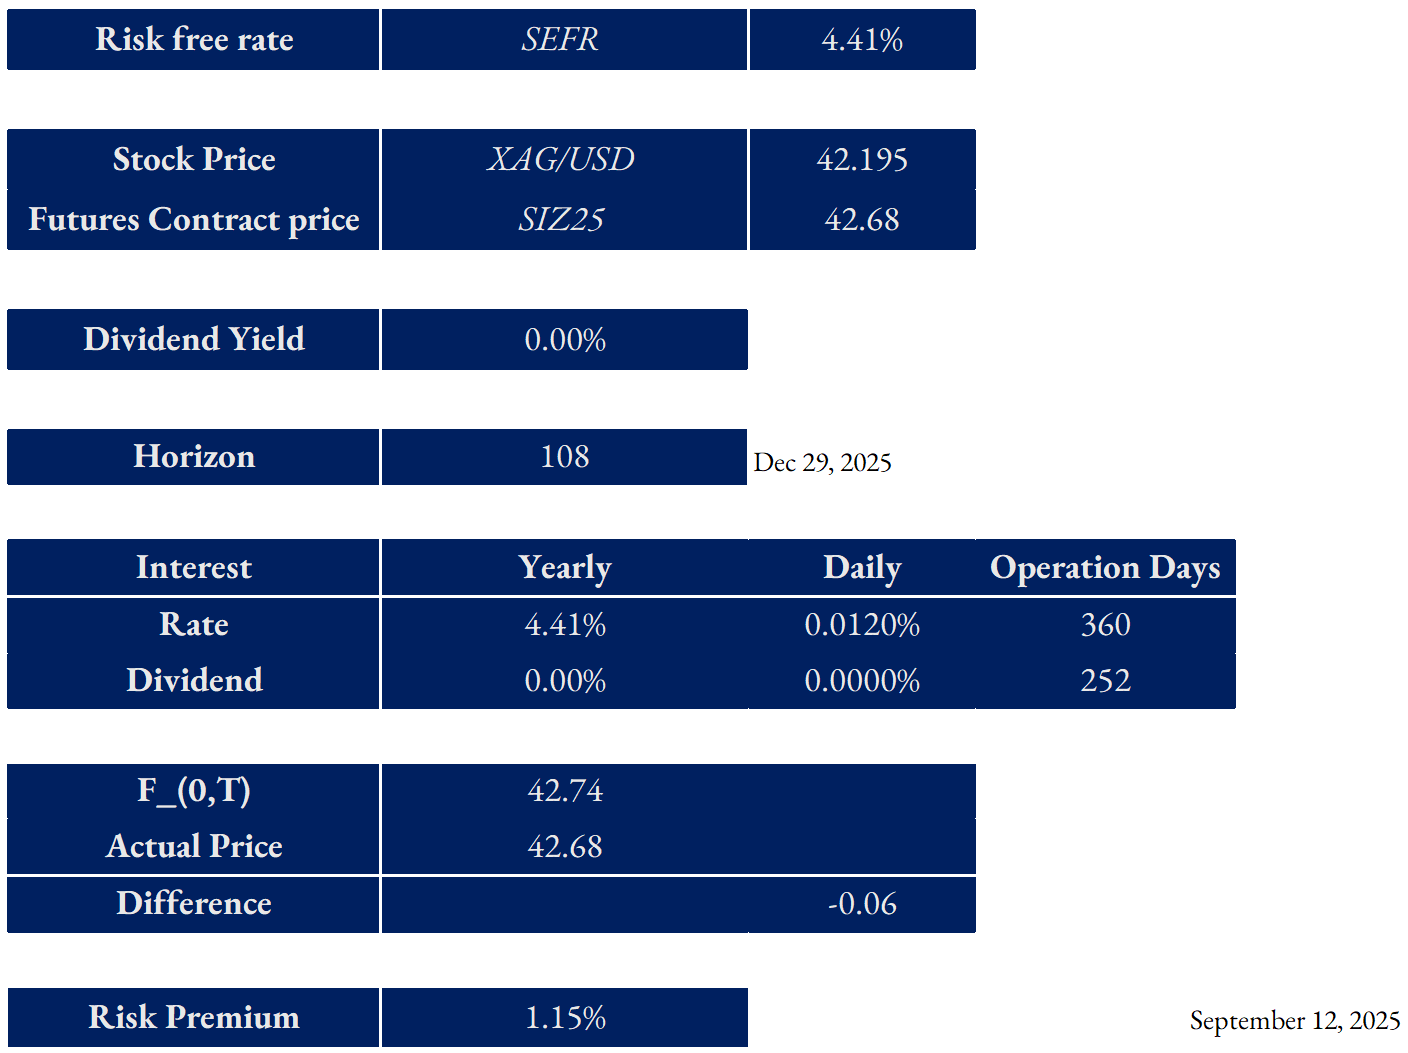
\includegraphics[width=0.7\textwidth]{figures/silver_pricing_one_day.png}
\caption{One-day pricing decomposition for SIZ25.}
\label{fig:silver_one_day}
\end{figure}


A small, but statistically meaningful, \emph{positive basis} is observed on \emph{September 12, 2025}: \(F=42.83>F^{*}=42.74\), i.e., a premium of \(\$0.09/\mathrm{oz}\) (18 ticks, \(\$450\) per 5{,}000-oz contract). With \(S=42.195\) and \(T=108/360\), the market-implied carry is
\[
c_{\mathrm{mkt}}=\frac{1}{T}\ln\!\frac{F}{S}=\frac{1}{0.30}\ln\!\frac{42.83}{42.195}\approx 4.97\% \ \text{p.a.}
\]
Given a funding benchmark \(r=4.41\%\), the net inventory term is obtained as
\[
u-l=c_{\mathrm{mkt}}-r\approx 0.60\%\ \text{p.a.}
\]
This decomposition is used to interpret the premium as \emph{slight contango}: financing and storage together exceed the lease (convenience) rate by a few basis points on an annualized basis, so the future prices above both spot and the pure-financing benchmark \(F^{*}=S\,e^{rT}\).


\paragraph{Why this is consistent with the news flow.}
Contemporaneous headlines emphasize (i) elevated spot levels on rising Fed-cut probabilities and a softer USD, (ii) ETF-related investor demand, and (iii) discussion of structural deficits. These elements are used to lift the \emph{subyacente} first; however, the futures price capitalizes financing and inventory over the next 108 days. The small, positive \(u-l\) indicates that, notwithstanding robust spot demand, lease rates have not surged enough to dominate funding and storage for this horizon. Adequate deliverable stocks, available storage, and year-end financing conditions can sustain a modest contango even as spot remains buoyant. Economically, this is read as a \emph{carry/liquidity configuration}, not as a dislocation or an arbitrage.




\medskip
\noindent\emph{Risk classification.} The premium sits well within typical no-arbitrage bands once bid–ask, exchange fees, collateral haircuts, and delivery frictions are recognized. Positioning should therefore emphasize curve-shape risk (carry and roll) rather than seeking to monetize an illusory mispricing.



\subsection{Weekly term-structure diagnostics (5–12 Sep 2025)}
Table-based evidence indicates a transition from \emph{mild backwardation} early in the week (negative Market \(-\) Theoretical) to \emph{mild contango} by Thursday–Friday (positive spreads). Interpreting \(u-l=\tfrac{1}{T}\ln(F/F^{*})\) with ACT/360:

\begin{figure}[h]
\centering
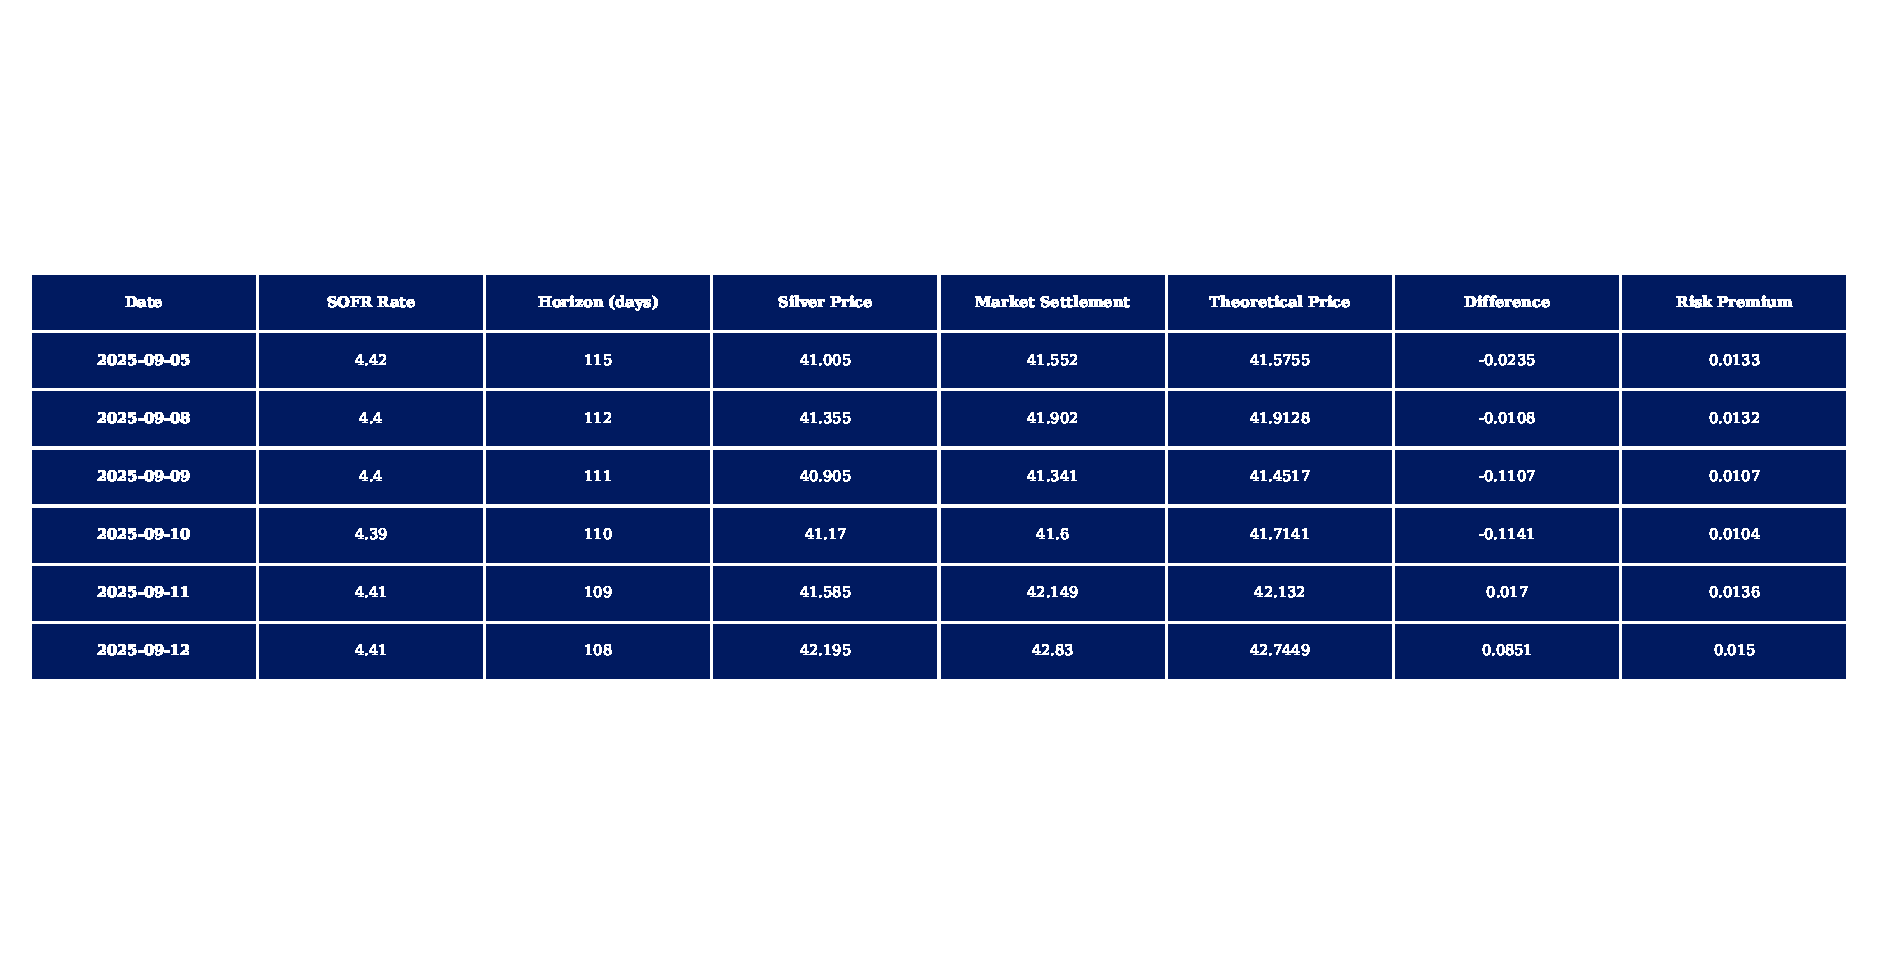
\includegraphics[width=\textwidth]{figures/silver_pricing_over_the_week.pdf}
\caption{Weekly evolution of Market \(-\) Theoretical and risk premium for SIZ25.}
\label{fig:silver_week}
\end{figure}

\begin{itemize}
  \item \textbf{9/5–9/10:} negative spreads (\(-\$0.02\) to \(-\$0.11\)/oz) imply \(l>r+u\): nearby inventory scarcity and/or elevated lease rates.
  \item \textbf{9/11–9/12:} positive spreads (\(+\$0.02\) to \(+\$0.09\)/oz) imply \(r+u>l\): easing tightness and/or stronger preference for futures exposure that capitalizes carry.
\end{itemize}
The “Risk Premium” \((F/S-1)\) remains small (≈1.06–1.50\%), dipping when spot outperforms and recovering as futures regain a modest premium. Economically, this premium summarizes carry (funding \(+\) storage \(-\) lease) and is best interpreted as a liquidity/carry effect rather than an arbitrage opportunity.

\begin{figure}[h]
\centering
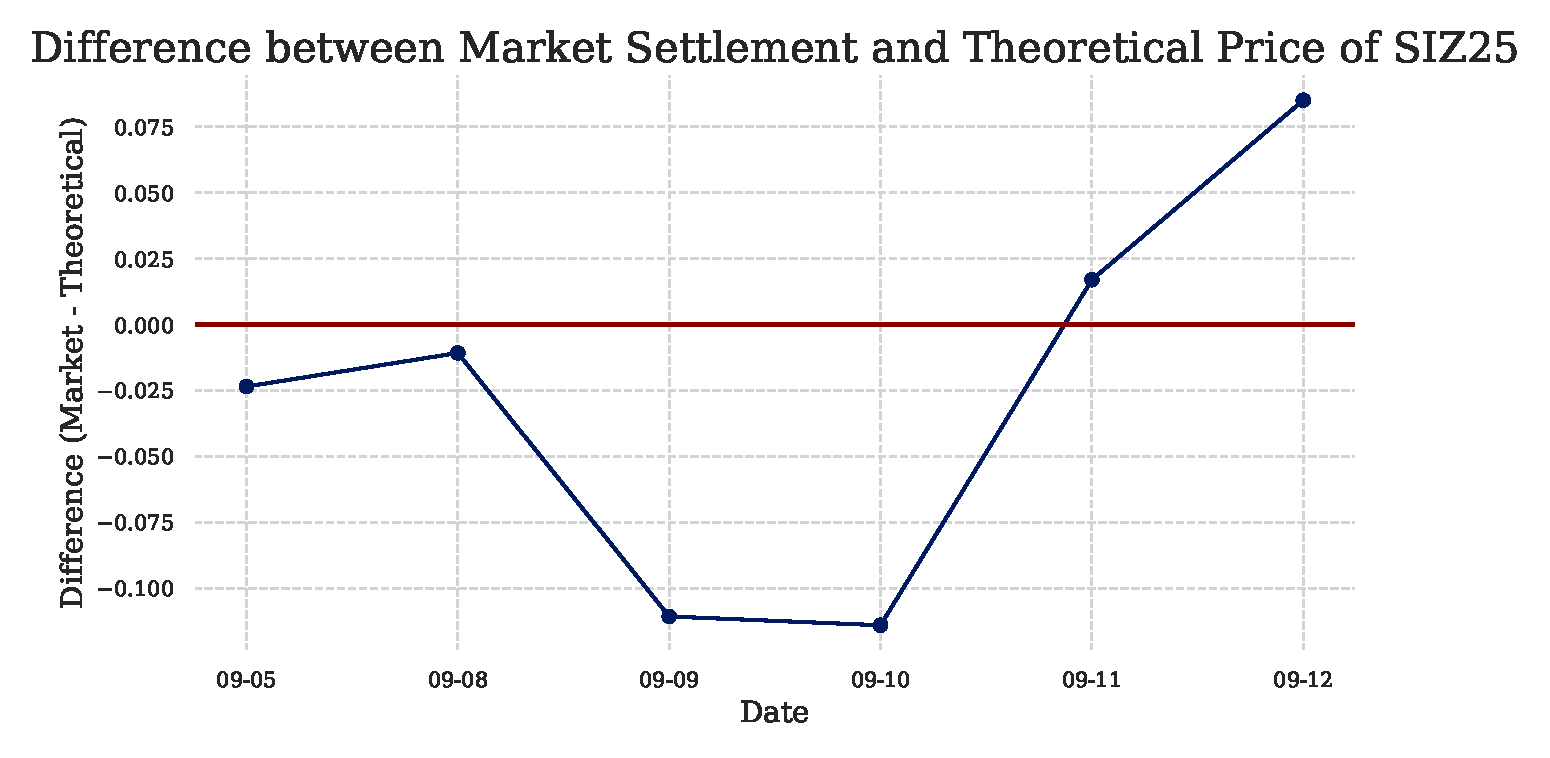
\includegraphics[width=0.7\textwidth]{figures/silver_difference.pdf}
\caption{Daily difference \(F-F^{*}\) and sign (backwardation vs.\ contango).}
\label{fig:silver_difference}
\end{figure}


The term structure transitions from \emph{mild backwardation} to \emph{mild contango} over the week. Early readings (\(F-F^{*}<0\)) are used to infer \(l>r+u\) for short horizons—consistent with transient tightness or elevated borrow in the physical market—while late-week readings (\(F-F^{*}>0\)) indicate \(r+u>l\) as funding and storage reassert dominance.

\paragraph{Day-by-day interpretation.}
Using \(u-l=\frac{1}{T}\ln(F/F^{*})\) (ACT/360; \(T\) declines from \(\sim 0.319\) to \(\sim 0.300\)):
\begin{itemize}
  \item \textbf{Fri 9/5:} \(F-F^{*}=-\$0.024\) \(\Rightarrow\) mild backwardation; \(u-l\approx-0.18\%\) p.a. It is used to read near-term inventory value as slightly elevated relative to carry.
  \item \textbf{Mon 9/8:} \(F-F^{*}=-\$0.011\) \(\Rightarrow\) mild backwardation; \(u-l\approx-0.08\%\) p.a. Tightness signal weakens; curve moves toward flat.
  \item \textbf{Tue 9/9:} \(F-F^{*}=-\$0.111\) \(\Rightarrow\) backwardation; \(u-l\approx-0.87\%\) p.a. A sharper spot-led impulse is used to widen the lease premium.
  \item \textbf{Wed 9/10:} \(F-F^{*}=-\$0.114\) \(\Rightarrow\) backwardation; \(u-l\approx-0.89\%\) p.a. Persistence of tightness; curve remains inverted at the front.
  \item \textbf{Thu 9/11:} \(F-F^{*}=+\$0.017\) \(\Rightarrow\) slight contango; \(u-l\approx+0.13\%\) p.a. The balance shifts; funding/storage begin to dominate.
  \item \textbf{Fri 9/12:} \(F-F^{*}=+\$0.085\) \(\Rightarrow\) contango; \(u-l\approx+0.66\%\) p.a. A normalized carry regime is used to characterize the close of the week.
\end{itemize}

\paragraph{Mechanistic drivers behind the flip.}
Three operational channels are typically implicated: (i) \emph{funding}—a rise in Fed-cut odds lowers expected discount rates but can steepen near-term collateral demand, dynamically affecting \(r\) relative to \(l\); (ii) \emph{inventory/warehouse}—refinery and warehouse flows can replenish deliverables, compressing lease premia; (iii) \emph{term demand}—investors may prefer futures exposure to defer physical handling, lifting \(F\) relative to spot once the initial spot-led surge abates. The observed risk premium \((F/S-1\approx 1.06\% \text{ to } 1.50\%)\) remains small; it is used as a summary statistic of carry rather than a tradable edge.

\subsection{Does this benefit Mexico? What should be done?}

\paragraph{Economic incidence for Mexico.}
As the leading global producer, Mexico is positioned to benefit from elevated spot and orderly term structure. The one-day contango and the week’s re-steepening are used to indicate that (i) near-term shipments monetize high spot realizations, and (ii) forward coverage can be implemented with manageable roll costs. FX pass-through matters: stronger silver improves terms of trade and is often peso-supportive, yet a stronger MXN reduces peso-denominated revenues unless currency risk is hedged.

\paragraph{Implications for investors (policy-neutral).}
\begin{enumerate}
  \item \textbf{Separate spot risk from curve risk.} It is used to treat price level (\(S\)) and roll/carry (\(F-S\), shape) as distinct. Long spot exposure benefits from the current level; futures strategies should model carry explicitly.
  \item \textbf{Hedge design.} For producers and MXN-based portfolios, it is used to pair metal hedges with FX hedges to stabilize peso cash flows. With slight contango, rolling short COMEX futures entails modest carry costs; in backwardation windows, rolls may be revenue-positive.
  \item \textbf{Tenor selection.} It is used to choose hedge tenors where \(u-l\) is stable and liquidity is deep (e.g., front two contract months), minimizing basis and execution risk.
  \item \textbf{Basis management.} Location and quality basis between London unallocated and COMEX deliverable bars should be monitored; treasury policy is used to set limits on basis drift and to pre-approve alternative hedging venues if needed.
\end{enumerate}

\paragraph{Implications for Mexico (policy and operating environment).}
\begin{enumerate}
  \item \textbf{Logistics and permitting reliability.} It is used to prioritize predictable permitting timelines and logistics corridors; stable, transparent processes compress location basis and reduce lease-rate spikes tied to bottlenecks.
  \item \textbf{Energy and power reliability.} Processing and refining require stable power; reliability improvements lower effective storage/operating costs \(u\), improving net margins across the cycle.
  \item \textbf{Market infrastructure and risk management.} It is used to encourage the adoption of standardized hedge programs (including FX overlays) among medium-size producers to align with best practices and reduce macro-volatility transmission to local cash flows.
  \item \textbf{Tax and royalty neutrality to hedging.} It is used to ensure that fiscal rules treat realized hedge outcomes neutrally relative to spot sales, avoiding distortions that discourage prudent risk transfer.
\end{enumerate}

\medskip
\noindent\emph{Synthesis.} The current configuration—high spot with slight, later-week contango—supports Mexican revenues while keeping roll costs contained. For investors, it is used to favor disciplined hedge-and-carry implementations that respect term-structure signals. For policymakers, reducing operational frictions and basis volatility enhances the capacity to translate favorable global prices into stable domestic income and investment.








\section{MXN/USD}

\subsection{Recent developments}
The peso entered mid-September 2025 near its strongest levels in over a year (\(\sim\)18.4–18.6 USD/MXN), supported by improved global risk appetite and rising odds of U.S. rate cuts. Market focus has been on: (i) the Federal Reserve path toward easing, which compresses U.S.–Mexico rate differentials and is typically MXN-supportive; (ii) Banxico’s gradualism, which preserves domestic carry; (iii) fiscal guidance that points to a narrower 2026 deficit; (iv) trade-policy proposals on autos that raise tail risks for the external sector; and (v) evolving Pemex support that can compress sovereign-linked risk premia if execution holds \citep{reuters_usdmxn_quote,reuters_mx_markets_11sep,reuters_mx_markets_12sep,reuters_fed_poll_2025,reuters_cenbank_graphic_2025,reuters_banxico_jun26_2025,banxico_calendar_2025,reuters_budget_2026_2025,reuters_tariffs_autos_2025,reuters_pemex_plan_2025,reuters_fitch_pemex_2025}.

\subsection{Spot \& futures}
Quoting follows CME convention: \emph{price = USD per MXN} (\$/MXN). To obtain the usual USD/MXN, invert. Spot (\(S\)) summarizes contemporaneous USD conditions and Mexico’s macro risk. Futures/forwards transfer FX risk across time under \emph{covered interest parity} (CIP):
\[
F = S\,e^{(r_{\mathrm{USD}}-r_{\mathrm{MXN}})T},
\]
with \(r_{\mathrm{USD}}\) a USD risk-free proxy (SOFR) and \(r_{\mathrm{MXN}}\) an MXN money-market rate. Because \(r_{\mathrm{MXN}}>r_{\mathrm{USD}}\) in typical regimes, \(\$/{\rm MXN}\) forwards price \emph{below} spot (equivalently, USD/MXN forwards \emph{above} spot). Deviations at very short tenors can reflect fixing times, holidays, and margin conventions; persistent deviations signal cross-currency basis \citep{bis_cip_2016,bis_cip_2024,frbny_sofr,frbny_sofr_index,cme_fx_overview,cme_mxn_product,cme_mxn_rulebook}.

\subsection{Mexico-linked implications}
FX levels and forward structure transmit into inflation, real incomes, and public finances. A firm MXN lowers traded-goods inflation and import costs, but compresses peso revenues for USD-earning sectors unless hedged. For the sovereign and large corporates, credible fiscal signals and Pemex risk reduction compress term premia that feed into longer-dated forwards. For real-money and corporate treasuries, CIP-implied discounts in \(\$/{\rm MXN}\) encode carry; hedge design should pair FX with underlying commodity or rate exposures to stabilize peso cash flows.

\subsection{Futures term structure (12 Sep 2025)}
\paragraph{Levels and shape.}
\[
\text{SEP-25 } \mathbf{0.054210}\ (\approx 18.447\ \text{USD/MXN})\ \rightarrow\ 
\text{DEC-25 } \mathbf{0.053700}\ (\approx 18.622)\ \rightarrow\ 
\text{MAR-26 } \mathbf{0.053170}\ (\approx 18.808)\ \rightarrow\ 
\text{SEP-26 } \mathbf{0.052100}\ (\approx 19.194)\ \rightarrow\
\text{DEC-26 } \mathbf{0.051550}\ (\approx 19.399)\ \rightarrow\
\text{MAR-27 } \mathbf{0.051010}\ (\approx 19.604).
\]
The curve is \emph{downward} in \(\$/{\rm MXN}\) (\(F<S\)), which corresponds to an \emph{upward} USD/MXN forward path. Annualized, SEP-25\(\to\)MAR-27 implies \(\sim 4.0\%\) p.a. MXN depreciation under CIP, consistent with \(r_{\mathrm{MXN}}-r_{\mathrm{USD}}\) for those tenors.

\paragraph{Microstructure.}
Activity concentrates in SEP- and DEC-25 (high volume and OI). Thinly traded months are marks-to-curve; treat small kinks with caution. With the curve sloping down in \(\$/{\rm MXN}\), long-MXN positions (long futures) face \emph{negative roll}, while short-MXN (long USD) earns forward carry.

\subsection{Interpretation of \texorpdfstring{MPZ25}{MPZ25} (one-day read)}
Using \(\$/{\rm MXN}\) spot \(S=0.05427\), front settlement \(F=0.05421\), and \(T=3/360\), the forward sits slightly \emph{below} spot by \(-6\times 10^{-5}\) \$/MXN (\(-0.11\%\) of spot). Under CIP:
\[
\frac{F}{S}=e^{(r_{\mathrm{USD}}-r_{\mathrm{MXN}})T}\;\Rightarrow\;
r_{\mathrm{MXN}}-r_{\mathrm{USD}}=\frac{1}{T}\ln\!\Big(\frac{S}{F}\Big).
\]
At such short horizons this annualizes to a large number due to \(T\ll 1\); economically it simply states \(r_{\mathrm{MXN}}>r_{\mathrm{USD}}\). The magnitude is well within no-arbitrage bands once day-counts, holiday effects, and bid–ask are recognized. Directionally, the sign matches the macro backdrop: Fed-easing expectations and Banxico gradualism favor a small forward \emph{discount} in \(\$/{\rm MXN}\).

\subsection{Weekly term-structure diagnostics (5–12 Sep 2025)}
\paragraph{Data (CME \$/MXN, ACT/360).}
\begin{center}
\begin{tabular}{lrrrrrr}
\toprule
Date & SOFR (\%) & \(T\) (days) & \(S\) & \(F\) & \(F^{*}=S e^{r_{\mathrm{USD}}T}\) & \(F{-}F^{*}\) \\
\midrule
2025-09-05 & 4.42 & 10 & 0.05343 & 0.05342 & 0.053494 & \(-7.4\times10^{-5}\) \\
2025-09-08 & 4.40 & 7  & 0.05359 & 0.05357 & 0.053635 & \(-6.5\times10^{-5}\) \\
2025-09-09 & 4.40 & 6  & 0.05370 & 0.05367 & 0.053739 & \(-6.9\times10^{-5}\) \\
2025-09-10 & 4.39 & 5  & 0.05377 & 0.05378 & 0.053802 & \(-2.2\times10^{-5}\) \\
2025-09-11 & 4.41 & 4  & 0.05417 & 0.05409 & 0.054196 & \(-1.06\times10^{-4}\) \\
2025-09-12 & 4.41 & 3  & 0.05427 & 0.05421 & 0.054290 & \(-8.0\times10^{-5}\) \\
\bottomrule
\end{tabular}
\end{center}

\paragraph{Read-through.}
\begin{itemize}
  \item \textbf{Sign and stability.} \(F<S\) on five of six days (tiny exception on 9/10), consistent with \(r_{\mathrm{MXN}}>r_{\mathrm{USD}}\). The daily forward discount vs.\ spot (\(F/S-1\)) ranges from about \(-0.02\%\) to \(-0.15\%\), small in economic terms yet directionally coherent.
  \item \textbf{Proper benchmark.} The negative \(F-F^{*}\) relative to \(F^{*}=S e^{r_{\mathrm{USD}}T}\) is \emph{expected} in FX because the correct fair value is CIP, \(S e^{(r_{\mathrm{USD}}-r_{\mathrm{MXN}})T}\). Using only USD funding overstates fair by the MXN carry component.
  \item \textbf{News linkage.} Fed-easing expectations (USD rates lower) and Banxico gradualism (MXN rates still high) maintain the forward \emph{discount} in \(\$/{\rm MXN}\). The small 9/10 blip (\(F\gtrsim S\)) is noise at \(T\leq 5\) days, plausibly from fixing and liquidity effects. Fiscal signals and Pemex support compress longer-dated premia but have little impact at one-week horizons; tariff headlines can widen risk premia episodically, yet the short-dated strip remained carry-driven.
\end{itemize}

\subsection{Does this benefit Mexico? What should be done?}
\paragraph{Assessment.}
A firm MXN with CIP-consistent forward discounts lowers imported-inflation pressure and stabilizes local financing conditions. For exporters and remitters, the stronger currency tightens peso revenues, which increases the importance of hedge overlays. The observed structure is benign: it rewards USD-based investors who hedge into MXN (positive carry) and allows domestic treasuries to pre-fund USD at predictable forward points.

\paragraph{Actions (policy-neutral investors).}
\begin{enumerate}
  \item \textbf{Separate level from carry.} Manage spot risk (USD/MXN) and carry risk (forward points) independently. Use short-dated forwards for cash-flow alignment; employ calendar rolls to manage carry.
  \item \textbf{Pair hedges.} Combine FX hedges with commodity or rate hedges where revenues or costs are joint (e.g., silver exporters hedging both XAG and MXN) to stabilize MXN cash flows.
  \item \textbf{Tenor discipline.} Favor liquid fronts (SEP, DEC) for execution; stair-step coverage to reduce fixing risk. Avoid annualizing micro-tenor signals.
\end{enumerate}

\paragraph{Actions (Mexico’s operating environment).}
\begin{enumerate}
  \item \textbf{Credible fiscal and Pemex execution.} Sustained consolidation and transparent Pemex support compress term premia embedded in longer-dated forwards.
  \item \textbf{Hedge accounting clarity.} Neutral tax and accounting treatment for FX hedges reduces frictions and encourages systematic risk transfer.
  \item \textbf{Market plumbing.} Robust local money markets and settlement infrastructure shrink cross-currency basis and improve CIP pass-through.
\end{enumerate}



\section{MXN/USD}
The exchange rate of the Mexican Peso (MXN) against the US Dollar (USD) is a crucial indicator of the Mexican economy and is influenced by a complex mix of domestic and international factors. One of the most important is the monetary policy of the US Federal Reserve (Fed). When the Fed raises its interest rates, the dollar strengthens, attracting investment into dollar-denominated assets and commonly causing a depreciation of the peso (i.e., it takes more pesos to buy one dollar). Similarly, interest rate decisions by the Bank of Mexico (Banxico) impact the exchange rate; higher rates can strengthen the peso by attracting foreign investment \citep{dallasfed_peso_2023,banxico_regional_2024}.

The overall state of the worldwide economy and investors' willingness to engage in risk are also pivotal determinants. The MXN is considered a "risk currency" or an "emerging market currency." During periods of global optimism and stability, investors often seek higher returns in emerging markets like Mexico, which appreciates the peso. Conversely, in times of uncertainty, geopolitical tension, or global recessions, investors seek safe-haven assets like the US dollar, triggering a massive sell-off of pesos and its depreciation \citep{bis_eme_internationalisation_2022}.

Internal factors and Mexico's economic situation play a fundamental role. Macroeconomic data such as GDP growth, the unemployment rate, inflation, and consumer confidence affect the perception of the country's stability. Furthermore, political events like elections, changes in fiscal policy (budgets, taxes), or the implementation of structural reforms can generate volatility in the exchange rate by impacting the confidence of foreign investors \citep{banxico_regional_2024}.

A historical event that exemplifies the MXN's extreme volatility was the Tequila Crisis in 1994. In December of that year, the Mexican government was forced to devalue the peso, which in a matter of days went from a fixed exchange rate of approximately 3.50 MXN per USD to over 7.00 MXN per USD—a devaluation of over 100\%. This crisis was triggered by a combination of a current account deficit, capital flight, and a crisis of confidence in economic policy \citep{imf_tequila_2012,yale_tequila_2012}.


\textbf{MPZ25} refers to the Mexican peso futures contract (MXN/USD quoted in \text{USD per 1 MXN}) that expires in December 2025. The current contract price shown is \(0.0537\) USD per MXN (equivalent to \(\sim 18.62\) MXN per USD). The spot used in the table is \(0.054266721\) USD per MXN (\(\sim 18.43\) MXN per USD) \citep{cme_mxn_product,cme_mxn_rulebook}.

This table compares the spot with what the futures price “should” be over \(94\) days using a USD risk-free rate (SEFR) of \(4.41\%\) and no extra costs/benefits. With those inputs, the theoretical price would be \(F_{0,T} \approx S_0(1+rT)\). For \(94\) days, \(rT \approx 0.0441 \times \frac{94}{360} = 0.01152\). Then \(F_{0,T} \approx 0.054266721 \times (1+0.01152) \approx \mathbf{0.05489}\) \citep{frbny_sofr}.\footnote{SEFR is commonly referred to as SOFR; data and methodology: \citep{frbny_sofr,frbny_sofr_index}.}
The market, however, is at \(0.0537\). This implies the futures price is \(0.00118\) below the theoretical value (\(\approx -2.17\%\) relative to that calculation).

In percentage terms versus spot, the table reports a “risk premium” of \(-1.04\%\), which comes from \(0.0537/0.054266721 - 1 \approx -1.04\%\).
The fair forward in FX follows covered interest parity: \(F \approx S_0 \frac{1 + r_{\text{USD}} T}{1 + r_{\text{MXN}} T}\) \citep{bis_cip_2016,bis_cip_2024}.

Since MXN rates are usually higher than USD rates, the MXN/USD forward is normally below the spot (i.e., the USD is expected to be more expensive in the future), which is exactly what your table shows. For example, if you assume an MXN rate around \(10\%\) annually for that tenor, the theoretical price is approximately \(F \approx 0.05427 \times \frac{1 + 0.0441 \cdot 94/360}{1 + 0.10 \cdot 94/360} \approx 0.0535\), very close to the \(0.0537\) in the market \citep{bis_cip_2016}.

\begin{figure}[h]
\centering
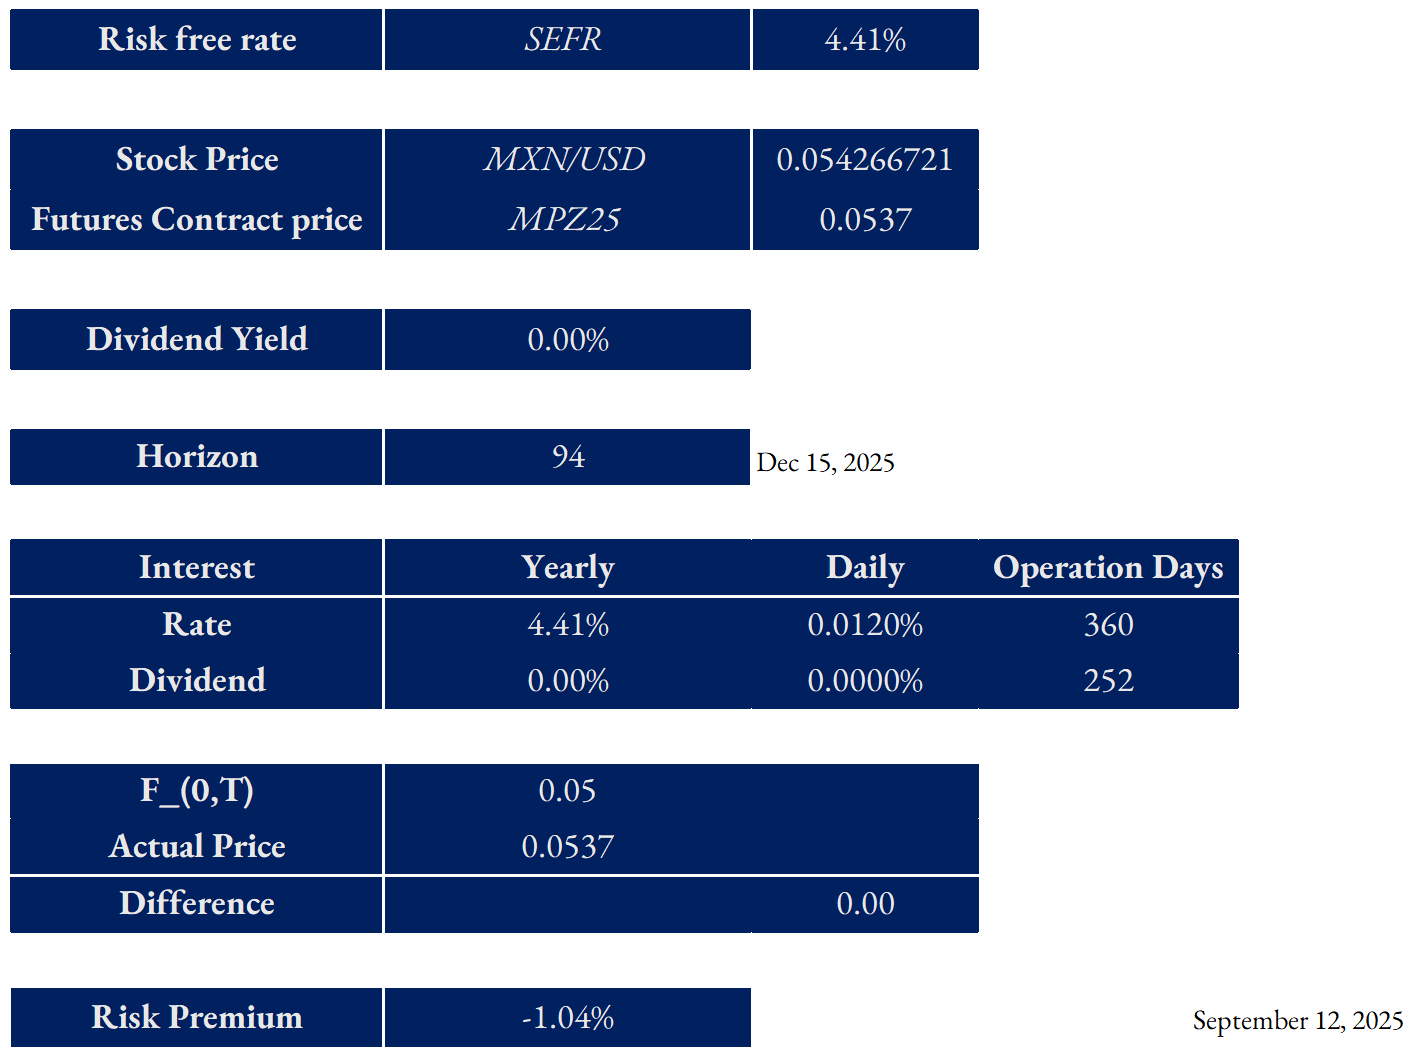
\includegraphics[width=0.7\textwidth]{figures/usdmxn.png}
\caption{Silver price series. Source: Investing.com.}
\end{figure}


\subsection{Futures term structure (12 Sep 2025)}
\paragraph{Interpretation uses CME quoting:} \emph{price = USD per MXN}. To compare with the usual \emph{USD/MXN}, invert.

\subsubsection*{Levels and curve}
\begin{itemize}
  \item \textbf{Fronts:} SEP-25 \textbf{0.054210} $\approx$ 18.447 USD/MXN; DEC-25 \textbf{0.053700} $\approx$ 18.622.
  \item \textbf{Outs:} MAR-26 \textbf{0.053170} $\approx$ 18.808; SEP-26 \textbf{0.052100} $\approx$ 19.194; DEC-26 \textbf{0.051550} $\approx$ 19.399; MAR-27 \textbf{0.051010} $\approx$ 19.604.
  \item \textbf{Shape:} \emph{Downward} in \$/MXN $\Rightarrow$ \emph{USD/MXN upward}. Implies \emph{gradual MXN depreciation}: $\approx$ \textbf{+6.3\%} from SEP-25 to MAR-27 ($\sim$\textbf{4.1\% p.a.}).
\end{itemize}

\subsubsection*{What the slope says}
\begin{itemize}
  \item Covered-interest-parity signal: with \textbf{MXN rates $>$ USD rates}, forwards price \textbf{MXN at a discount}. The $\sim$3.7--4.1\% annualized fall in \$/MXN from SEP$\rightarrow$DEC-25 and out the curve is consistent with that rate differential, not a pure macro ``view.''
\end{itemize}

\subsubsection*{Daily move}
\begin{itemize}
  \item \textbf{SEP-25 change +0.000120:} \$/MXN \textbf{+0.22\%}. Inverted, \textbf{USD/MXN $-0.22\%$} $\rightarrow$ \textbf{MXN strengthened} on the day.
  \item \textbf{DEC-25 change +0.000120} similar sign and size.
\end{itemize}

\subsubsection*{Liquidity and microstructure}
\begin{itemize}
  \item \textbf{Very active:} \textbf{Est. volume 82,475}, \textbf{OI 267,710}. Concentration in \textbf{DEC-25 (53,457 vol, 170,511 OI)} and \textbf{SEP-25 (29,018 vol, 97,132 OI)}.
  \item ``B/A'' marks are quotes (bid/ask), not prints. Zero volume months are \emph{marks to curve}; treat small kinks there cautiously.
\end{itemize}

\subsubsection*{Trading reads}
\begin{itemize}
  \item \textbf{Direction:} Long future = long MXN (profits if \$/MXN rises / USD/MXN falls).
  \item \textbf{Carry/roll:} With downward \$/MXN curve, \emph{long-MXN has negative roll}; \emph{short-MXN (long USD)} earns forward carry.
  \item \textbf{Macro sensitivity:} A faster-than-priced narrowing of the \emph{Banxico--Fed} gap flattens the curve (backs up in \$/MXN; downs in USD/MXN). Policy surprises dominate short-dated moves; rate-differential path drives the back.
\end{itemize}

\subsubsection{USD/MXN: recent news and pricing implications}
\paragraph{Spot context.}
As of mid-September 2025, USD/MXN trades near 18.45, the peso having reached its strongest levels in over a year amid improved global risk sentiment and lower U.S. rate expectations \citep{reuters_usdmxn_quote,reuters_mx_markets_11sep,reuters_mx_markets_12sep}.

\paragraph{Key developments.}
\begin{enumerate}
  \item \textbf{Federal Reserve path.} A 25 bp cut at the September meeting is widely expected, with markets pricing additional easing by year end; this lowers U.S. rate differentials against MXN and is typically peso-supportive \citep{reuters_fed_poll_2025,reuters_cenbank_graphic_2025}. 
  \item \textbf{Banxico stance and calendar.} Banxico reduced the policy rate to 8.0\% on June 26 and has signaled a gradual path thereafter; the next decision falls on a Thursday at 13:00 CST per the published calendar. A slower easing cadence preserves carry in MXN \citep{reuters_banxico_jun26_2025,banxico_calendar_2025}. 
  \item \textbf{Fiscal guidance.} The draft 2026 budget foresees a narrower deficit (4.1\%/GDP) and includes so-called ``healthy taxes''; improved fiscal optics tend to compress sovereign risk premia and modestly support MXN \citep{reuters_budget_2026_2025}. 
  \item \textbf{Trade policy.} A plan to impose 50\% tariffs on vehicles from non-FTA countries is being advanced; tighter trade measures can weigh on Mexico’s external sector and raise risk premia, which is MXN-negative \citep{reuters_tariffs_autos_2025}. 
  \item \textbf{Pemex credit and sovereign linkages.} A government plan to reduce Pemex debt and a rating upgrade to BB reflect stronger support; improved Pemex credit metrics can narrow Mexico’s risk premium and aid MXN, though execution risk remains \citep{reuters_pemex_plan_2025,reuters_fitch_pemex_2025}. 
\end{enumerate}

\paragraph{Mapping to spot and futures.}
For spot, U.S. rate cuts and steady domestic carry are associated with USD weakness and MXN strength; adverse trade shocks or Pemex slippage work in the opposite direction. For futures, interest-rate parity is used:
\[
F \approx S \, e^{(r_{\mathrm{USD}} - r_{\mathrm{MXN}})T},
\]
so a downward shift in the Fed path (\(r_{\mathrm{USD}}\downarrow\)) is used to lower \(F\) relative to \(S\), while a faster Banxico easing (\(r_{\mathrm{MXN}}\downarrow\)) is used to raise \(F\). Fiscal consolidation and Pemex support compress risk premia that are often embedded in longer-dated forwards, while tariff risks and global-growth shocks are used to widen them \citep{cme_mxn_quotes,cme_fx_overview}.


\paragraph{Measurement.} A small \textbf{positive basis} is observed: the futures price exceeds the theoretical cost-of-carry value by \textbf{20.64 points} $(F=61{,}840 > F^{\*}=61{,}819.36)$, which corresponds to \textbf{0.07\%} on the index. In equity-index pricing, $F^{\*}=S\,e^{(r-q)T}$ is used; therefore a positive $F-F^{\*}$ indicates that the \textbf{market-implied carry} $\hat{c} = \tfrac{1}{T}\ln(F/S)$ is slightly \textbf{above} the model’s $(r-q)$, equivalently that the \textbf{effective dividend drag} expected to expiry is a bit lower than assumed (or that marginal funding is a bit higher).

\paragraph{Interpretation with the news backdrop.} The recent macro mix—Fed easing expectations, supportive global risk appetite, a relatively firm MXN, and locally gradual Banxico guidance—creates a setting in which index futures demand is used to obtain fast beta exposure and dividend-timing risk is perceived as limited. Under these conditions, a \textbf{modestly richer future} vs.\ fair is consistent with: (i) pro-risk positioning that lifts $F$ marginally, (ii) slightly lower expected dividends before expiry, and (iii) liquidity/carry effects as equities trade near highs. The signal is small and lies within typical no-arbitrage frictions; it is read as a \textbf{mild, pro-risk tilt} rather than a standalone mispricing.

\subsection{Futures term structure (Sep 12, 2025)}

\subsection{Interpretation of \texorpdfstring{MPU25}{MPU25} (one-day read)}
\subsection{Weekly term-structure diagnostics (5–12 Sep 2025)}




\newpage
\section{TIIE}


The TIIE is today the central reference for the cost of overnight peso funding; it is the base price of money used by banks and firms to set interest on loans, bonds, and other instruments. It is estimated with one-day wholesale repo operations settled at INDEVAL, with government or equivalent collateral, and with banks and broker-dealers as participants. Based on these transactions, Banxico reports a representative daily rate and, in addition, \textbf{composition indices} that accumulate daily factors over business or calendar days and ``forward compounded'' versions useful for contracts that require explicit capitalization. The result reflects what actually happened in the market \citep{banxico_methodology,banxico_indices}.

At the CME, the futures contract allows trading the compounded rate; Futures price = 100 − expected compounded F-TIIE (annualized) over the contract’s reference period. By convention it is quoted as \textbf{Index = 100 - 100R}. For example, today the rate is 8.0126\% and its CME futures price for the TIEU25 contract maturing on September 30, 2025 is 92.28

Where For a monthly TIE with $D$ calendar days and daily F-TIIE fixes $r_i$ applying to $d_i$ days each:

  $$
  R=\Bigg(\prod_{i}^n\big(1+\tfrac{1}{360}r_i\big)-1\Bigg)\cdot \tfrac{360}{n},\qquad
  {\text{Futures price}=100-R}
  $$

In this work it is assumed expect F-TIIE to be flat for the next horizon days. Then the compounded average annualizes back to

$$
R=\Bigg(\big(1+\tfrac{1}{360}r_i\big)^n-1\Bigg)\cdot \tfrac{360}{n}.
$$

For example, today at September 12, the rate is 8.0126\% for 18 days to expire on September 30, 2025. Then  

\begin{align*}
  F^* &= 100 - 100\cdot \Bigg(\big(1+\tfrac{1}{360}(8.0126)\big)^{18}-1\Bigg)\cdot \tfrac{360}{18}. \\
  & = 91.97
\end{align*}


A \textbf{+1 bp} change in the expected annualized rate moves the futures \textbf{−1 tick bp}, \textbf{P\&L = −MXN 200/contract}; the \textbf{minimum tick 0.5 bp = MXN 100}.

\begin{center}
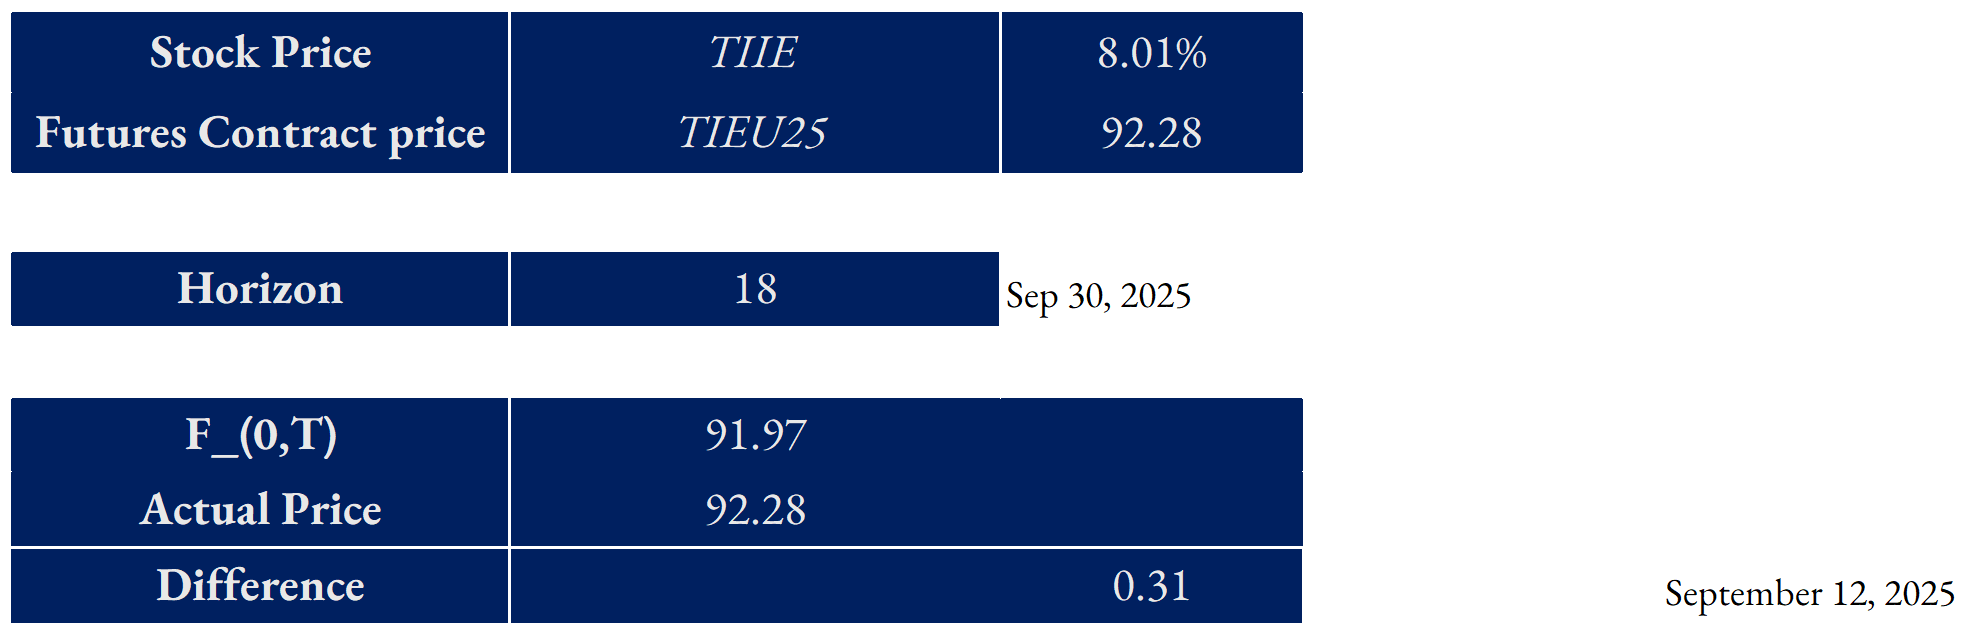
\includegraphics[width=0.5\textwidth]{figures/tiie_pricing_sep12.png}
\end{center}

A \textbf{positive basis in price} is observed: the \textbf{futures contract} $F=92.28$ is \textbf{above} the theoretical fair value $F^*=92.16$. The \textbf{implied monthly market rate} is therefore about \textbf{12 bps lower} than the model rate, since the market is discounting a \textbf{lower average TIEU25} for the remainder of the month than assumed by the fair value that is, a smoother downward path of rates. In other words, the expectation is for average rates to drift lower. Under the futures convention \textbf{Index = 100 - 100·R}, a \textbf{higher price implies a lower implied rate}. 

From this perspective, the market is effectively pricing a rate of:
\begin{itemize}
  \item \textbf{Market-implied}: $R_{\text{mkt}} = \tfrac{100-92.28}{100} = \mathbf{7.72\%}$.
  \item \textbf{Model (fair)}: $R_{\text{mod}} = \tfrac{100-92.16}{100} = \mathbf{7.84\%}$.
\end{itemize}

\textbf{Current level} (spot TIIE 28d $\approx 8.01\%$): since 12 days have already accrued at $\sim8.01\%$ and 18 days remain, in order for the monthly average to settle at $7.72\%$, the remaining path must evolve near \textbf{7.49\%}. This indicates a market signal of \textbf{gradual softening} of the TIEU25 for the rest of the month.

It is important to emphasize that this reflects an \textbf{expectation of the monthly average}, not a guarantee of an immediate policy cut. The 7.72\% already incorporates carry and the days elapsed; it may be achieved through a steady mild decline or fluctuations around $\sim7.5$--$7.6\%$. If the basis were negative (price $<$ fair), the interpretation would be reversed: an \textbf{implicit rise} in the expected average.

This could be caused by the fact that the Federal Reserve (Fed) is considering rate cuts because the labor market shows signs of cooling, with job creation revised down and unemployment slightly higher, which reduces wage and aggregate demand pressures \citep{reuters2025a}. In addition, inflation, while still above 2\%, shows some moderation and anchored expectations, which allows room for maneuver without eroding credibility \citep{ycharts2025}. At the same time, the policy rate remains in restrictive territory, above neutral, creating the risk of excessive slowdown \citep{ycharts2025}. Moreover, the U.S. economy faces stagnation signals and weaker growth, while the global environment increases vulnerabilities \citep{reuters2025b}. Finally, institutions such as the IMF have noted that the Fed has space to ease its stance given the deterioration in labor dynamics \citep{reuters2025c}, and Powell himself has acknowledged employment risks as an argument to open the door to cuts \citep{reuters2025d}.

If the Fed starts cutting and the peso remains stable, the market usually anticipates that the rate $R$ will decline; then the TIIE futures price rises. The approximate profit or loss per contract is 
\[
\Delta \text{P\&L} \approx 50{,}000 \times \Delta \text{Index} \quad \text{MXN}
\]
\citep{banxico2023,cme2025a,cme2025b,reuters2025a}. 

The process can be described as follows:

\begin{enumerate}
    \item New information arrives. For example, lower inflation signals in the U.S. and Fed guidance toward \textbf{consecutive cuts} \citep{reuters2025}.
    \item Very short-term USD rates fall. Dollar funding becomes cheaper and the expected path shifts downward.
    \item Global financial conditions ease. Lower risk aversion and often a weaker USD reduce imported inflationary pressure in Mexico.
    \item Banxico assesses the local picture. If inflation and the exchange rate cooperate, the market anticipates local cuts with a \textbf{lag} relative to the Fed. That \textbf{expected path} is what matters for derivatives.
    \item The expected TIEU25 for the quarter decreases. The compounded TIEU25 of the period, $R$, falls if each daily ``drop'' is slightly smaller.
    \item The futures price rises. By convention, \textbf{lower $R \Rightarrow$ higher Index}, because Index $= 100 - R$. A change of $-25$ bp in $R$ implies $+\!0.25$ index points.
\end{enumerate}

As an example, suppose the market expects an annualized compounded rate of $R = 10.00\%$. The futures contract trades near $100 - 10.00 = 90.00$. If, after cut guidance, consensus shifts to $R = 9.75\%$, the price would be 90.25. The approximate variation for a long contract is:

\[
\Delta \text{P\&L} \approx (90.25 - 90.00)\times 50{,}000 = \textbf{12{,}500 \ \text{MXN}}.
\]

Of course, this is not always the case, for several reasons:

\begin{itemize}
    \item \textbf{Local decoupling.} A rebound in Mexican inflation or a peso depreciation may lead Banxico to delay or cut less; $R$ falls less and the futures price rises less or corrects.
    \item \textbf{Technical factors.} Term premiums, paper supply, repositioning, or calendar effects. The compounding methodology extends the last published rate on weekends and holidays, introducing small differences across months and quarters and a \textbf{basis} between what you want to hedge and what the contract settles \citep{cme2025a,cme2025b}.
\end{itemize}

\subsection{TIIE futures term structure (as of Sep 12, 2025)}
Reading rule: \textbf{Price = 100 $-$ implied annualized F-TIIE}. So each settle gives an implied rate $R$.

Key reads from your strip (implied $R=100-\text{Settle}$):

\begin{itemize}
  \item \textbf{Term-structure}: downward. Market prices \textbf{easing} $\approx -91$ bp from \textbf{SEP-25 7.740\%} to \textbf{AUG-27 6.830\%}, then a small \textbf{rebound +17.5 bp} into \textbf{SEP-27 7.005\%}.
  \item \textbf{Front vs late-2025}: big steps early $\rightarrow$ expected cuts concentrated in \textbf{Q4-25}:
    \begin{itemize}
      \item SEP-25 \textbf{7.740\%}, OCT-25 \textbf{7.535\%} ($-20.5$ bp m/m), NOV-25 \textbf{7.350\%} ($-18.5$ bp), DEC-25 \textbf{7.240\%}.
    \end{itemize}
  \item \textbf{2026}: flatter, small humps.
    \begin{itemize}
      \item JUN-26 \textbf{7.015\%}, DEC-26 \textbf{6.980\%}. Micro kinks suggest meeting-month risk or illiquidity marks.
    \end{itemize}
  \item \textbf{2027}: trough around \textbf{6.83--6.85\%} through AUG, then \textbf{SEP-27 up to 7.005\%}. Read as mild re-steepening/term premium rather than a new cycle.
  \item \textbf{Liquidity signal}: Est. Volume = 0 almost everywhere; OI material only in \textbf{OCT-25 (492)} and \textbf{SEP-25 (120)}. Most far maturities are \textbf{marks to curve}, not traded prints. Treat kinks cautiously.
  \item \textbf{Microstructure}: each contract settles to the \textbf{monthly compounded overnight F-TIIE}, linearly annualized. A single policy cut inside a month drags that month’s average, but not one-for-one with the policy rate.
  \item \textbf{Carry math}: 1 bp move in implied $R$ = \textbf{MXN 200/contract}. Long futures wins if the market reprices to a \textbf{lower} implied rate; short wins if repriced \textbf{higher}.
  \item \textbf{Spot check vs today’s fix}: if today F-TIIE $\approx$ \textbf{8.0126\%}, then \textbf{SEP-25 at 7.740\%} implies the remaining September days are expected \textbf{below today’s fix} on average.
\end{itemize}

\textbf{Actionable take:}
\begin{itemize}
  \item Express a \textbf{cuts view} by going \textbf{long} the near contracts you believe are too high in $R$ (too low in price).
  \item Hedge path risk by spreading adjacent months if your view is about \textbf{timing} of cuts, not total magnitude.
  \item Use the OI cluster (SEP/OCT-25) for tighter execution; far months are curve proxies.
\end{itemize}

Signal quality. With zero volume, “Change” is weak evidence of shifting expectations. Use swap/OIS quotes or nearby active months to infer policy path.

Tactics. Prefer limit orders and the months with OI; consider calendar spreads for timing views; for size or precision use OTC MXN OIS vs F-TIIE.



\subsection{TIIE futures term structure (as of Sep 8, 2025)}


Read as \textbf{price = 100 $-$ implied annualized F-TIIE}. Your settles imply these rates:

\begin{itemize}
  \item \textbf{SEP-25 92.2500 $\rightarrow$ 7.7500\%} ($\Delta$price $-0.0100$ $\Rightarrow$ rate \textbf{+1.0 bp} d/d)
  \item \textbf{OCT-25 92.4600 $\rightarrow$ 7.5400\%} (unch)
  \item \textbf{NOV-25 92.6600 $\rightarrow$ 7.3400\%} (\textbf{+1.5 bp lower} d/d in rate since price $+0.0150$)
  \item \textbf{DEC-25 92.7600 $\rightarrow$ 7.2400\%} (price $+0.0050$ $\Rightarrow$ rate $-0.5$ bp)
  \item \textbf{JAN-26 92.7300 $\rightarrow$ 7.2700\%}, \textbf{FEB-26 92.7850 $\rightarrow$ 7.2150\%}, \textbf{MAR-26 92.8650 $\rightarrow$ 7.1350\%}
  \item \textbf{Apr--Aug-26 $\approx$ 7.06--7.03\%}, \textbf{late-26 $\approx$ 7.10$\rightarrow$7.06\%}
  \item \textbf{Jan--Aug-27 7.05$\rightarrow$6.935\%}, then \textbf{SEP-27 92.8450 $\rightarrow$ 7.1550\%} (kink up)
\end{itemize}

\textbf{Observations:}
\begin{itemize}
  \item \textbf{Curve shape:} Clear easing path from \textbf{7.75\% (Sep-25)} toward \textbf{$\sim$6.94\% (Aug-27)}, then a \textbf{re-steepening} in \textbf{Sep-27}. That last jump likely reflects illiquidity or a marking artifact, not a firm macro call.
  \item \textbf{Cut timing:} Steep drops into \textbf{Nov--Dec-25} imply cuts clustered in Q4-25. Monthly comp means a 25 bp policy cut mid-month pulls the month’s average by $\approx$12--13 bp, not 25 bp.
  \item \textbf{Microstructure:} \textbf{Estimated volume = 2} (only \textbf{NOV-25} traded). \textbf{DEC-25 ``92.7650B''} is a \textbf{bid}, not a trade. Almost all other lines are \textbf{clearing marks}. Treat daily ``Change'' as curve marking, not price discovery.
  \item \textbf{Liquidity:} \textbf{OI 653} total, concentrated in \textbf{SEP-25 (120)} and \textbf{OCT-25 (492)}. Far maturities with OI=0 are curve placeholders.
  \item \textbf{Day-over-day signal:} Front months barely moved in rate terms ($\pm$0--1.5 bp). Far months were marked higher in price by \textbf{3--10+ ticks} ($\approx$1.5--5 bp lower in implied rate), consistent with gentle long-end bull-flattening.
  \item \textbf{Relative to today’s fix (8.0126\%):} Near contracts imply the remainder of Sep-25 averages \textbf{below 8\%}, consistent with expected easing path already underway.
  \item \textbf{P\&L units:} \textbf{1 bp} change in implied rate = \textbf{MXN 200/contract}; min tick \textbf{0.5 bp = MXN 100}. With \textbf{OI 653}, market DV01 $\approx$ \textbf{MXN 130.6k per bp}.
  \item \textbf{Tactics:} Express a view in \textbf{SEP/OCT-25} where OI exists. Use \textbf{calendar spreads (e.g., OCT/NOV, NOV/DEC)} if your view is about \textbf{cut timing}. Treat \textbf{Sep-27 kink} as low-quality unless volume appears.
\end{itemize}


\subsection{Interpretation of \texorpdfstring{TIEU25}{TIEU25} (one-day read)}
\subsection{Weekly term-structure diagnostics (5–12 Sep 2025)}

\section{TIIE}

\subsection{Recent developments}
Policy signaling and inflation data point to a gradual easing cycle in Mexico, conditioned by external monetary policy and exchange-rate dynamics. On \emph{Aug 7, 2025}, Banco de México lowered the policy rate to \textbf{7.75\%} in a divided vote, noting headline inflation around the target band and weak activity \citep{reuters_banxico_cut_aug25,banxico_mps_aug7_2025}. Into mid-September, softer U.S.\ labor data raised the probability of a Federal Reserve cut at the September meeting, weakening the USD and easing global financial conditions \citep{reuters_global_cuts_sep11a,reuters_global_cuts_sep11b}. MXN strengthened and Mexican equities set record highs, consistent with easier external conditions \citep{reuters_mxn_sept15}. These forces are typically transmitted to the local front end: \emph{Funding TIIE} (F-TIIE) fixes in the near term, and the \emph{term structure} of implied monthly compounded F-TIIE via futures \citep{frbny_sofr_page,fred_sofr}.

\subsection{Spot \& futures}
The \emph{Overnight Funding TIIE} is a transaction-based reference rate calculated from peso repo trades settled at INDEVAL; Banxico also publishes compounding indices on business and calendar bases that allow exact accrual over arbitrary periods \citep{banxico_f_tiie_method,banxico_indices_page,banxico_on_method_en}. CME’s \emph{Mexican Funding TIIE (Monthly)} futures settle to the annualized compounded average of each day’s F-TIIE over the contract month, quoted as
\[
\textbf{Index} \equiv 100 - 100\,R_{\text{comp}},
\]
with ACT/360 convention and final settlement equal to \(100 - R_{\text{month}}\) \citep{cme_tiie_monthly_overview,cme_tiie_monthly_specs,cme_tiie_monthly_method,cme_tiie_quarterly_overview}. Hence, a higher futures price implies a lower \emph{implied} compounded monthly rate, and a 1~bp change in the implied rate corresponds to \(\pm \textbf{MXN 200}\) per contract (tick \(=0.5\)~bp \(=\) MXN~100) \citep{cme_tiie_monthly_specs}.

\subsection{Mexico-linked implications}
Because F-TIIE underpins Bondes~F and cascades into bank funding curves, the monthly compounded futures are used to transfer near-term policy-path risk from balance sheets to the market \citep{cme_tiie_monthly_overview,cme_ftiie_article}. Easing expectations raise the index (lower implied \(R\)), delivering mark-to-market gains to longs; conversely, stickier inflation or MXN weakness can reprice the front months lower. The curve’s \emph{shape} encodes the distribution of expected Banxico cuts across calendar months; microstructure matters because some listed months are \emph{marks to curve} rather than traded prints.

\paragraph{Transmission map.}
Monthly F--TIIE futures translate into prices (i) the expected path of Banco de México’s policy stance, (ii) wholesale MXN funding dynamics, and (iii) external shocks (Fed, USD). By convention,
\[
\text{Futures Price} \equiv 100 - 100\,R_{\text{comp}},
\]
so higher price $\Leftrightarrow$ lower implied monthly compounded rate. Contract sensitivity: $\Delta \mathrm{P\&L} \approx 50{,}000 \times \Delta \text{Index}$ MXN per contract; $1$ bp in $R$ $\Rightarrow \pm$ MXN $200$; minimum tick $=0.5$ bp $=$ MXN $100$.

\paragraph{Banks (ALM and net interest margins).}
\begin{itemize}
  \item \textbf{NIM mechanics.} Funding costs typically adjust faster than asset yields on variable-rate books. A first-order margin response is
  \[
  \Delta \mathrm{NIM} \simeq w_A\,\beta_A\,\Delta r \;-\; w_L\,\beta_L\,\Delta r,
  \]
  where $w_A,w_L$ are asset/liability weights and $\beta_{A,L}$ are repricing betas. If $\beta_L>\beta_A$ initially, easing can widen NIM before convergence.
  \item \textbf{Hedging.} Long monthly F--TIIE futures (benefit from price up) protect margins in a cuts repricing; shorts protect against a hawkish reversal. Timing risk is better expressed with \emph{calendar spreads} (e.g., OCT/NOV) than outright notional.
  \item \textbf{Basis risk.} Futures settle to the \emph{monthly} compounded overnight index (ACT/360), while effective funding mixes business-day patterns, liquidity buffers, and idiosyncratic spreads. Manage this basis via limits, backtesting, and mapping rules from F--TIIE to transfer-pricing curves.
\end{itemize}

\paragraph{Pension funds, insurers, and mutual funds.}
\begin{itemize}
  \item \textbf{Tactical duration and carry.} Falling implied $R$ supports long-carry in Mbonos/Bondes F. Monthly futures provide a clean front-end overlay to \emph{nowcast} policy moves without disturbing strategic allocations.
  \item \textbf{Execution.} Concentrate orders in high-OI near months; predefine roll windows and size caps to mitigate market impact.
\end{itemize}

\paragraph{Corporates and treasuries.}
\begin{itemize}
  \item \textbf{Financing cost.} Easing reduces MXN floating-rate expense and expands debt capacity. Align hedges (long monthly F--TIIE) with months of peak cash interest outflow.
  \item \textbf{Dollarized revenues.} For USD-revenue firms with MXN liabilities, pair long F--TIIE with FX hedges to stabilize MXN margins.
\end{itemize}

\paragraph{Households and consumption.}
\begin{itemize}
  \item Variable-rate credit costs ease gradually (cards, payroll, auto). Mortgage transmission is slower. The debt-service relief supports consumption with lags; monitor inflation risks via MXN.
\end{itemize}

\paragraph{Sovereign and state-owned enterprises.}
\begin{itemize}
  \item \textbf{Rollover costs.} Lower front-end rates reduce near-term funding expense and anchor Bondes F auctions. Staggered hedging across liquid months minimizes slippage and basis volatility.
  \item \textbf{Governance.} Neutral tax and accounting treatment of hedge outcomes preserves incentives for prudent use of monthly futures.
\end{itemize}

\paragraph{Money-market and microstructure considerations.}
\begin{itemize}
  \item \textbf{Path extraction.} The monthly futures curve encodes \emph{when} and \emph{how much} easing is priced. Kinks with low open interest are often \emph{marks}, not firm views.
  \item \textbf{Conventions.} Weekend/holiday compounding extends the last fix and can generate small inter-month differences; document ACT/360 assumptions in internal pricing policy.
\end{itemize}

\paragraph{External channel and MXN.}
\begin{itemize}
  \item Fed cuts typically ease global financial conditions and weaken USD. MXN appreciation lowers tradables inflation and permits Banxico to ease with less risk to expectations. Adverse USD shocks invert this logic and can delay the local cycle.
\end{itemize}

\paragraph{Operational scenarios.}
\begin{itemize}
  \item \textbf{Faster-than-expected cuts.} Futures prices rise in the front cluster; longs benefit; liability managers gain relief. Tighten limits on F--TIIE vs.\ internal funding basis and re-estimate repricing betas.
  \item \textbf{Delayed or data-dependent path.} Prices fall; shorts protect NIM and margins. Use \emph{calendar spreads} to express “delay” without overcommitting gross notional.
  \item \textbf{FX shock (MXN weaker).} Harder easing path; hedge both $R$ and FX to bound MXN P\&L.
\end{itemize}

\paragraph{Synthesized recommendations.}
\begin{enumerate}
  \item Separate \emph{level risk} (implied $R$) from \emph{timing risk} (monthly compounding). Use front contracts for direction and adjacent spreads for timing.
  \item Execute in high-OI nodes; manage and report the basis between monthly F--TIIE and internal funding metrics.
  \item Integrate rate and FX hedges where revenue/cost currencies differ; adopt standardized hedge accounting to preserve fiscal neutrality.
\end{enumerate}


\subsection{Futures term structure (12 Sep 2025)}
Rule of thumb for reading: \(\text{Implied }R = 100 - \text{Settle}\). The observed strip (CME monthly) shows a clear easing path from the front:
\[
\text{SEP-25 } \sim \mathbf{7.74\%}\ \to\ \text{OCT-25 } \sim \mathbf{7.53\%}\ \to\ \text{NOV-25 } \sim \mathbf{7.40\%}\ \to\ \text{DEC-25 } \sim \mathbf{7.37\%},
\]
flattening into 2026 near \(7.0\%\), troughing around \(6.83\%\) by mid–late 2027, then a mild re-steepening \citep{cme_tiie_monthly_quotes}. This configuration is consistent with clustered cuts over \(\text{Q4-2025}\) followed by a slower cadence, not a sharp overshoot. Liquidity is concentrated in the nearest listed months; far maturities should be treated as curve marks \citep{cme_tiie_monthly_overview,cme_tiie_monthly_quotes}.

\subsection{Interpretation of \texorpdfstring{TIEU25}{TIEU25} (one-day read, 12 Sep 2025)}
Using your inputs for \emph{Sep 12}:
\[
\text{Settle} = \mathbf{93.035}\ \Rightarrow\ R_{\text{mkt}}=\mathbf{6.965\%}.
\]
Your \emph{model} fair \((F^{*})\) built by extending the latest daily fix across the horizon implies
\[
F^{*}=\mathbf{91.6369}\quad\Rightarrow\quad R_{\text{mod}}=\mathbf{8.363\%}.
\]
Hence, the \emph{price basis} \(F-F^{*}=\mathbf{+1.398}\) index points maps to an \emph{expected-path gap} of \(\sim\mathbf{140}\)~bp: the market discounts a monthly-compounded average materially below the flat-at-spot benchmark. Economically, this is a \emph{front-loaded easing} signal: with days already accrued near \(8.01\%\), the remaining path must average lower to deliver \(6.97\%\) for the target month \citep{banxico_on_method_en,cme_tiie_monthly_method}.

\subsection{Weekly term-structure diagnostics (5–12 Sep 2025)}
\paragraph{Data snapshot.} Your weekly table shows \(\text{Settle}\uparrow\) from \(\mathbf{92.855}\) to \(\mathbf{93.035}\) as the horizon decays \(390\to383\) days; implied rate falls \(\mathbf{7.145\%\to6.965\%}\) (\(\approx \mathbf{-18}\)~bp). The model fair \(F^{*}\) is stable near \(91.62\)–\(91.64\), so the basis widens from \(\sim\!+1.24\) to \(\sim\!+1.40\) points.

\paragraph{Interpretation.} The \emph{direction} (higher price, lower implied \(R\)) aligns with global news that boosted odds of a Fed cut and softened the USD \citep{reuters_global_cuts_sep11a,reuters_global_cuts_sep11b}. That external easing channel, plus Banxico’s August 25~bp cut and guidance, rationalizes a modest bull-flattening of the near curve \citep{reuters_banxico_cut_aug25,banxico_mps_aug7_2025}. The persistent positive basis relative to your flat-at-spot model encodes \(\sim\)1.3–1.4~pp of cumulative easing over the next year. Day-count decay (ACT/360) explains why the \(|F-F^{*}|\) drifts only slowly even as the view strengthens.

\paragraph{Microstructure note.} CME monthly F-TIIE shows concentrated open interest in the front cluster; far-month marks are less informative intraday. For higher-fidelity path inference, cross-check with MXN OIS and Banxico-dated IRS where available.

\subsection{Does this benefit Mexico? What should be done?}
\textbf{Banks.} A lower expected path compresses deposit and wholesale funding costs first; asset yields on variable-rate loans reprice with lags. Net interest margins narrow unless liabilities reprice faster. Use front-month \textbf{short} F-TIIE futures to protect NIM against a hawkish repricing; use \textbf{long} positions if liability relief is the objective \citep{cme_ftiie_article}.

\textbf{Corporates.} For MXN debt, easing lowers interest expense and raises debt capacity. Treasury teams should pair MXN OIS or monthly F-TIIE longs with FX overlays if revenues are USD-linked.

\textbf{Households/consumers.} Variable-rate credit costs ease gradually; mortgage and durable-goods financing become more affordable. Inflation risks from MXN swings should be monitored.

\textbf{Sovereign/Pemes.} Lower front-end rates reduce rollover costs. Transparent hedge governance can lock favorable funding while avoiding concentration in a single month.

\textbf{Tactics.} 
(i) Express a \emph{cuts} view by going \textbf{long} near-month contracts; 
(ii) express \emph{timing} via calendar spreads (e.g., OCT/NOV) because monthly comp averages dilute within-month decisions; 
(iii) manage execution in months with open interest; 
(iv) track MXN and U.S.\ rates as primary catalysts.

\medskip
\noindent\emph{Synthesis.} The weekly drift higher in price and the sustained positive basis versus a flat-at-spot model are consistent with an easing path concentrated in \(\text{Q4-2025}\) and moderating thereafter. For Mexico, this configuration supports a measured decline in funding costs without destabilizing curve kinks. Implementation should separate \emph{level} risk (the implied rate \(R\)) from \emph{timing} risk (month-by-month comp effects) and align hedge tenors with liquidity nodes.



\section{IPC}

\subsection{Recent developments}
Mexico’s benchmark \emph{S\&P/BMV IPC} printed fresh highs into \emph{12 Sep 2025} as global risk appetite improved on rising Fed-easing probabilities and a firm peso backdrop \citep{reuters_ipc_record_2025,reuters_usdmxn_quote}. Local conditions remain supportive but gradual: Banxico’s pace of easing is measured amid stable inflation expectations, while fiscal messaging and quasi-sovereign considerations (Pemex) shape equity risk premia and multiples \citep{bloomberg_mx_inflation_2025,mnd_inflation_band_2025,reuters_budget_2025,reuters_pemex_plan_2025}. Trade-policy headlines (e.g., prospective auto tariffs) interact with the nearshoring narrative and the industrial complex, generating sectoral rotations \citep{reuters_tariffs_china_autos_2025,reuters_border_jobs_2025}.

\subsection{Spot \& futures}
The IPC is float-adjusted, market-cap weighted under published rules \citep{spdj_ipc_page,spdj_bmv_methodology}. Spot index levels reflect contemporaneous earnings, discount rates, and MXN conditions; futures on MexDer transfer price risk across time. The fair-value relation
\[
F_T = S_0\,e^{(r-q)T}
\]
is used, where \(r\) is the relevant funding rate and \(q\) the dividend yield over \([0,T]\). In practice, thin trading in deferred IPC maturities and dividend-timing uncertainty add microstructure noise around this benchmark \citep{mexder_ipc_fut}. In the accompanying tables, SOFR is used as the working \(r\) for consistency across assets; ideally an MXN funding curve would be applied for precision. This choice does not alter the qualitative reading of the week’s carry dynamics.

\subsection{Mexico-linked implications}
Equity levels and futures carry transmit into financing conditions for issuers, pension/wealth portfolios, and the hedging cost of domestic asset managers. A steeper contango (\(r>q\)) raises the “cost of carry” for long futures exposure but eases the roll for short index overlays; compressing contango (via lower \(r\) or higher \(q\)) does the opposite. Policy credibility (fiscal/Pemex) and Banxico guidance compress risk premia, supporting spot while also affecting the slope through the \(r\) channel.

\paragraph{Transmission channels.}
The IPC level and its futures carry transmit to Mexico’s real and financial economy through five primary channels:
\begin{enumerate}
  \item \textbf{Sovereign and macro risk premia.} Credible fiscal guidance and Pemex execution compress sovereign spreads, supporting equity multiples and lowering the \emph{required} discount rate; this improves spot and, via the rate channel, can compress \(r-q\) on the strip \citep{reuters_budget_2025,reuters_pemex_plan_2025}.
  \item \textbf{FX and external balance.} Pro–risk global conditions and favorable terms of trade strengthen MXN, which reduces imported inflation and supports real income, but dampens exporters’ MXN revenues unless FX is hedged; IPC futures help neutralize equity beta while FX overlays manage currency co-movement \citep{reuters_usdmxn_quote}.
  \item \textbf{Corporate financing and issuance windows.} Higher spot and lower equity risk premia improve primary/secondary equity issuance conditions; modest contango (\(r>q\)) raises the carry cost of long index overlays used by issuers and asset managers to warehouse market exposure while deals are executed \citep{spdj_ipc_page,spdj_bmv_methodology}.
  \item \textbf{Pension and wealth portfolios.} Afores and local managers use IPC futures to control beta around rebalances; with \(r-q\approx 3\%\) p.a., maintaining long overlays has a measurable but manageable carry cost, which falls if Banxico eases in line with disinflation \citep{bloomberg_mx_inflation_2025,mnd_inflation_band_2025}.
  \item \textbf{Sectoral earnings sensitivity.} Trade-policy shocks (e.g., prospective auto tariffs) and nearshoring dynamics rotate earnings leadership across consumer, industrial, and materials sectors; derivatives are used to implement temporary tilts while stock-specific catalysts arrive \citep{reuters_tariffs_china_autos_2025,reuters_border_jobs_2025}.
\end{enumerate}

\paragraph{Derivatives-specific incidence.}
\begin{itemize}
  \item \textbf{Carry and roll.} With modest contango, long futures positions incur negative roll yield absent price appreciation; short overlays benefit. If Fed cuts arrive and Banxico follows gradually, \(r\downarrow\) compresses \(r-q\) and reduces long-carry drag \citep{reuters_ipc_record_2025}.
  \item \textbf{Dividend timing.} Near-expiry basis is sensitive to ex-dividend dates of large constituents; it is used to align rolls with the dividend calendar to minimize slippage. The one-year strip embeds an \emph{expected} \(q\)-path that can diverge from realized distributions.
  \item \textbf{Liquidity concentration.} Trading and OI cluster in the front contract; far maturities are marks. Hedgers should stage coverage along liquid nodes to reduce execution and basis risk \citep{mexder_ipc_fut}.
\end{itemize}

\paragraph{Sectoral and policy linkages.}
\begin{itemize}
  \item \textbf{Industrials/nearshoring.} Improved logistics and regulatory clarity raise earnings durability and support higher multiples; IPC futures hedge interim market swings while capacity is built.
  \item \textbf{Energy and quasi-sovereign complex.} Transparent Pemex funding plans lower tail risk and compress the equity risk premium market-wide; slope effects come via the rate channel \citep{reuters_pemex_plan_2025}.
  \item \textbf{Trade regime.} Auto-tariff decisions reprice supply chains and consumer prices, altering margins; managers use index futures plus sector tilts to bridge event risk \citep{reuters_tariffs_china_autos_2025}.
\end{itemize}

\paragraph{Actionable playbook (Mexico focus).}
\begin{enumerate}
  \item \textbf{Issuers and treasuries.} Use spot strength to pre-hedge equity-linked issuance with short IPC overlays; collapse overlays post-allocation to lock funding at improved valuations.
  \item \textbf{Asset owners (Afores).} Separate beta and carry: maintain target equity beta with front IPC futures and manage \(r-q\) via calendar spreads if a slope compression is anticipated from Fed/Banxico sequencing.
  \item \textbf{FX integration.} Pair IPC overlays with USD/MXN hedges when liability currency or benchmark is MXN, recognizing that pro–risk rallies can strengthen MXN and alter MXN-denominated tracking.
  \item \textbf{Policy levers.} Reinforce fiscal signaling and Pemex transparency to lower macro risk premia; deepen far-month futures liquidity to reduce basis noise and improve hedge effectiveness across horizons.
\end{enumerate}

\paragraph{Scenario map (link to news).}
\begin{description}
  \item[\textit{Faster Fed easing, gradual Banxico.}] Spot supported; \(r\downarrow\) compresses \(r-q\), flattening contango. Bias: favor long beta with lighter carry drag; calendar flatteners (long near/short far) gain.
  \item[\textit{Tariff escalation or growth scare.}] Spot vulnerability; MXN may weaken. Bias: protective short overlays; pair with FX hedges. \(q\) risk rises if dividend guidance is cut; \(r-q\) may widen if local rates stay firm.
  \item[\textit{Pemex/fiscal credibility gains.}] Risk premia compress; issuance windows improve; slope impact via lower \(r\). Bias: opportunistic issuance and overlay reduction; extend hedge tenors as basis stability improves.
\end{description}

\paragraph{Monitoring set.}
Track (i) implied \(r-q(T)=\frac{1}{T}\ln(F_T/S_0)\) across tenors, (ii) front-month basis vs.\ ex-dividend calendar, (iii) slope changes around Banxico/Fed events, and (iv) liquidity/roll metrics in the front two contracts. These diagnostics are used to translate news into implementable positioning while maintaining MXN-aware risk control.


\subsection{Futures term structure (as of 12 Sep 2025)}
\paragraph{Shape and slope.}
The strip is in \emph{modest contango}. From \textbf{SEP-25} to \textbf{SEP-26} settlements rise by \(\sim 2{,}009\) points. The one-year slope is
\[
\frac{F_{1\mathrm{Y}}}{F_{0}}-1 \approx \frac{63{,}767}{61{,}758}-1 \approx \mathbf{3.25\%},
\qquad
\Rightarrow\quad r-q \approx \ln\!\Big(\frac{F_{1\mathrm{Y}}}{S_0}\Big)\approx \mathbf{3.20\%\ \text{p.a.}}
\]
under risk-neutral pricing. Interpretation: funding exceeds expected dividends by \(\sim 3.2\%\) over the next year.

\paragraph{Level move.}
The curve shifted up almost in parallel on the session (\(+0.23\%\) front; \(+0.30\%\)–\(0.32\%\) deferred), a spot-led move consistent with the news backdrop, with limited change in \((r-q)\).

\paragraph{Liquidity note.}
Trading concentrates in \textbf{SEP-25}; far maturities showed near-zero volume and OI. Deferred marks should be treated as carry proxies, not high-conviction levels.

\subsection{Interpretation of one day (12 Sep 2025)}
A small \emph{positive basis} is observed: \(F=61{,}840>F^{*}=61{,}819.36\), a premium of \(20.64\) points (\(\sim \mathbf{0.07\%}\)). In the fair-value map \(F_T=S_0 e^{(r-q)T}\), this is read as a market-implied carry \(\hat c=\frac{1}{T}\ln(F/S_0)\) that is marginally above the model’s \((r-q)\), i.e., a slightly lower effective dividend drag or marginally higher funding over the remaining days. Economically, it signals a \emph{modest pro-risk tilt} amid supportive global conditions, not an arbitrage.

\subsection{Weekly term-structure diagnostics (5–12 Sep 2025)}
\paragraph{Observed path.}
Across the week, the futures premium to spot \((F/S_0-1)\) drifts from \(\mathbf{+0.40\%}\) (9/5) to \(\mathbf{-0.07\%}\) (9/12), with interim readings of \(+0.27\%\), \(+0.13\%\), \(+0.32\%\), and \(+0.10\%\). The market–model gap (\(F-F^{*}\)) narrows mechanically as \(T\) shortens, while daily \((F,S_0)\) co-move with equities’ risk-on tone.

\paragraph{Carry inference.}
Using the horizon-specific reading \(r-q=\frac{1}{T}\ln(F/S_0)\), the \emph{implied} \((r-q)\) oscillates around small positive values early week and turns slightly negative into 9/12 as \(F\) slips below \(S_0\) on very short \(T\). This is consistent with (i) rising proximity to dividend accruals and (ii) session-specific microstructure (basis and last/settle timing). Given the short horizons, annualized inferences are volatile; the one-year strip discussed above is the appropriate gauge for the structural \(r-q\) of \(\sim 3.2\%\).

\paragraph{News linkage.}
The pattern matches the backdrop: Fed-cut expectations lift spot and compress forward premia; Banxico’s gradualism maintains positive carry at longer maturities; dividend timing and index-lending dynamics dominate the front-days basis. Net effect: a curve that is \emph{up in level} with \emph{modest contango} intact, while near-expiry prints toggle around flat as ex-dividend proximity and microstructure bite.

\subsection{Does this benefit Mexico? What should be done? How does it affect it?}
\paragraph{Benefit.}
Higher spot IPC levels support wealth effects and lower equity risk premia, aiding funding conditions for issuers. A modest contango implies limited carry costs for maintaining long futures exposure and stable hedging for pension funds and domestic managers.

\paragraph{Investor actions (policy-neutral).}
\begin{enumerate}
  \item \emph{Decompose risks.} Manage spot beta and carry separately. Use front contracts for beta; use calendar spreads to express views on \((r-q)\) compression if Fed cuts and dividend seasonality are expected to flatten the slope.
  \item \emph{Hedge design.} For MXN-based portfolios, pair IPC futures with USD/MXN overlays when relevant to stabilize peso-denominated performance, recognizing the FX–equity interaction in risk-off episodes.
  \item \emph{Dividend timing.} Near-expiry basis is sensitive to ex-div schedules. Align rebalancing and roll dates with the dividend calendar to minimize slippage.
\end{enumerate}

\paragraph{Policy and operating implications.}
\begin{enumerate}
  \item \emph{Signal clarity.} Transparent fiscal guidance and Pemex execution reduce sovereign risk premia, supporting spot and compressing \((r-q)\) via the rate channel.
  \item \emph{Market depth.} Measures that deepen far-month liquidity reduce basis noise and improve hedge effectiveness across horizons.
  \item \emph{Macro mix.} A gradual Banxico path consistent with nominal anchors maintains credible carry while avoiding abrupt slope shifts that raise hedging costs.
\end{enumerate}

\medskip
\noindent\emph{Synthesis.} Into mid-September 2025, the IPC exhibits a spot-led advance with a modest, orderly contango. One-day and weekly diagnostics are coherent with the news flow: supportive global rates and steady local policy compress front premia while leaving the one-year \(r-q\) near \(\sim 3.2\%\). For Mexico, this configuration improves funding optics and portfolio transmission; for investors, it favors disciplined beta plus carry-aware implementation; for policymakers, credibility and market depth are the levers that translate favorable conditions into durable risk premia compression.


\section{IPC}

The S\&P/BMV IPC is the flagship index of the Mexican equity market, designed to measure the performance of the largest and most liquid stocks listed on the Bolsa Mexicana de Valores (BMV). It is float-adjusted, market-cap weighted, and maintained under published rules with regular rebalances \citep{spdj_ipc_page,spdj_bmv_methodology}.

\paragraph{Derivatives and implementation.}
Exposure and hedging are available via IPC futures listed at MexDer; these contracts are designed to manage equity-market risk tied to the Mexican market benchmark \citep{mexder_ipc_fut}.

\paragraph{Nowcasting the next move: macro–market linkages.}
As of \emph{September 12, 2025}, the IPC printed a new all-time high near 61{,}900, supported by risk-on flows as markets price imminent Fed cuts; the peso hovered around 18.4 per USD \citep{reuters_ipc_record_2025,reuters_usdmxn_quote}. This backdrop interacts with Mexico’s local cycle and policy mix:

\begin{enumerate}
    \item \textbf{Fed trajectory and global risk appetite.} Rising odds of a September Fed cut lowered U.S. yields and improved EM risk sentiment, historically supportive for Mexico’s equities and currency \citep{reuters_ipc_record_2025}.
    \item \textbf{Banxico path and inflation.} Recent data show headline inflation ticking up, prompting a slower easing cadence even as inflation expectations remain near target; net effect: supportive discount-rate impulse, but gradual \citep{bloomberg_mx_inflation_2025,mnd_inflation_band_2025}.
    \item \textbf{Fiscal stance and sovereign risk.} The 2026 budget narrative points to a slightly narrower deficit after 2025, with attention on execution and quasi-sovereign exposures (e.g., Pemex) that shape risk premia and equity multiples \citep{reuters_budget_2025,reuters_pemex_plan_2025}.
    \item \textbf{Trade/industrial policy shocks.} Proposed 50\% tariffs on vehicles from non-FTA countries would rewire EV/auto pricing in Mexico, with potential rotation across consumer, industrial, and materials names via supply-chain and price-elasticity channels \citep{reuters_tariffs_china_autos_2025}.
    \item \textbf{Nearshoring vs.\ frictions.} The medium-term nearshoring thesis coexists with cyclical frictions; recent reports of border-maquiladora job losses tied to U.S. tariff dynamics illustrate downside risk to industrial earnings momentum \citep{reuters_border_jobs_2025}.
\end{enumerate}

\paragraph{Base case and risks.}
Netting these forces, the near-term base case is a \emph{carry-and-liquidity-supported drift} while the Fed turns, tempered by Banxico’s gradualism and policy noise. Upside risks: faster global disinflation and credible domestic fiscal/Pemex execution that compress risk premia. Downside risks: renewed inflation pressure, sharper USD strength, escalation of tariff frictions, or disappointing growth that erodes earnings leverage \citep{reuters_ipc_record_2025,bloomberg_mx_inflation_2025,reuters_budget_2025,reuters_pemex_plan_2025,reuters_tariffs_china_autos_2025}.

\begin{figure}[h]
\centering
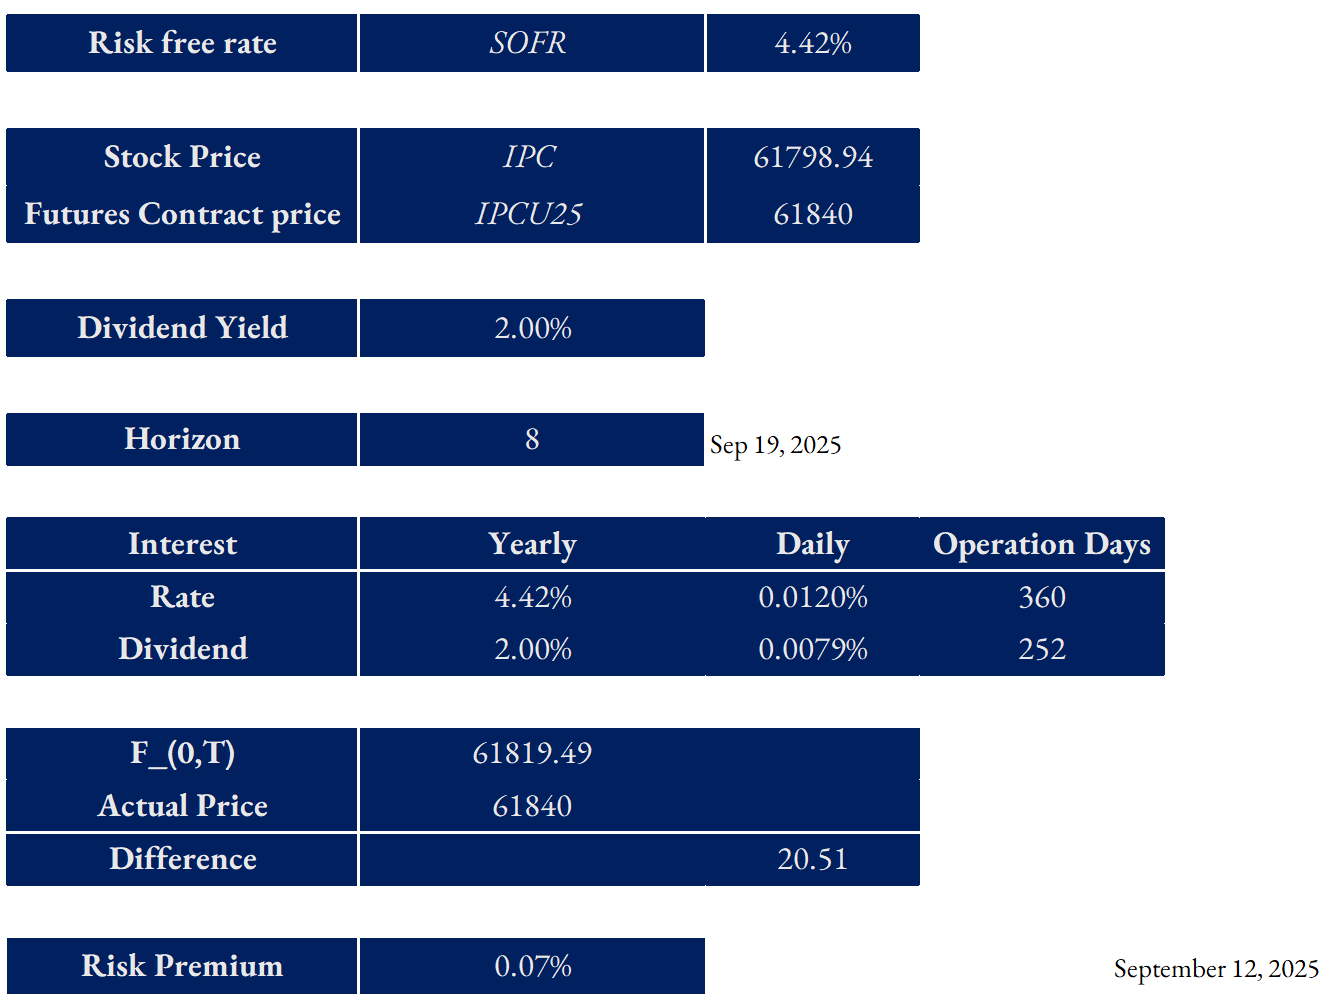
\includegraphics[width=0.7\textwidth]{figures/ipc.png}
\caption{Silver price series. Source: Investing.com.}
\end{figure}

\paragraph{Measurement.} A small \textbf{positive basis} is observed: the futures price exceeds the theoretical value by \textbf{20.64 points} $(F=61{,}840 > F^{*}=61{,}819.36)$. In equity-index futures priced via the cost-of-carry relation $F^{*}=S\,e^{(r-q)T}$, a positive $F-F^{*}$ is interpreted as a market-implied carry $\hat{c} = \tfrac{1}{T}\ln(F/S)$ that is \textbf{slightly above} the model’s $(r-q)$. Equivalently, the market is embedding a \textbf{lower effective dividend yield} over the remaining horizon (or marginally higher funding) than the one used in the model. Expressed on the underlying, the premium equals \textbf{$\approx 0.07\%$}, which is economically small and typically falls within no-arbitrage frictions (bid–ask, financing haircuts, dividend-timing uncertainty, and LAST vs SETTLE timing).

\paragraph{Interpretation with the news background.} In a setting where risk appetite is supported by anticipated Fed easing, a firm MXN, and benign local discount-rate dynamics, a \textbf{slightly richer future} is consistent with: (i) \textbf{long-demand in futures} to gain rapid benchmark exposure, (ii) \textbf{temporarily lower dividend-drag} expected between now and expiry, and (iii) \textbf{carry-and-liquidity effects} when equity rallies compress index lending spreads. The signal is therefore read as a \textbf{modest, pro-risk tilt}—not a standalone arbitrage—indicating that the market prices a marginally easier near-term environment for Mexican equities than implied by the model inputs.

\subsection{Futures term structure (as of Sep 12, 2025)}

The IPC futures term structure as of September 12, 2025, is shown in the Appendix. The front contract (SEP-25) expires on September 19, 2025. (\hyperref[fig:ipc_settlements]{View the Appendix for the future price settlements}).

Read rule: equity index future. \textbf{Fair value $F_T = S_0\,e^{(r-q)T}$} where $r$ is the MXN funding rate and $q$ is the IPC dividend yield over $[0,T]$. Price is in index points.

Key reads from your strip:

\begin{itemize}
  \item \textbf{Liquidity:} Only \textbf{SEP-25} traded. \textbf{Est. volume 196}, \textbf{OI 65}. \textbf{DEC-25+} show \textbf{0 volume, 0 OI}---mostly \textbf{marks}, not prints. The ``B/A'' on SEP means best bid/ask quotes, not trades.
  \item \textbf{Session move:} SEP-25 \textbf{+144 pts} $\approx$ \textbf{+0.23\%}; deferred marks \textbf{+195--200 pts} $\approx$ \textbf{+0.30--0.32\%}. Curve shifted up in parallel, slightly larger at the back.
  \item \textbf{Term-structure:} Contango. Settles rise from \textbf{61758 (SEP-25)} to \textbf{63767 (SEP-26)}. Quarterly steps: \textbf{+531, +492, +493, +493}. From front to 1-yr out: \textbf{+2009 pts} $\rightarrow$ slope $\approx$
  \[
    \frac{F_{1Y}}{F_{0}}-1 \approx \frac{63767}{61758}-1 \approx 3.25\%
    \quad\Rightarrow\quad
    r-q \approx \ln\left(\frac{63767}{61758}\right)\approx 3.20\%~\text{p.a.}
  \]
  Interpretation: under risk-neutral pricing the market implies \textbf{funding $>$ dividend yield by $\sim$3.2\%} over the next year.
  \item \textbf{Carry/basis mechanics:} With weeks to SEP expiry, $F-S$ should be small and tends to $S\,(r-q)\,T$ at short $T$. Positive contango is consistent with $r>q$. It is \emph{not} an equity growth forecast; it is cost-of-carry.
  \item \textbf{Sensitivity to Banxico:} Cuts lower $r$. All else equal, contango compresses and deferred futures cheapen vs.\ near. Calendar \emph{long SEP / short DEC or MAR} benefits if $r-q$ falls faster than implied.
  \item \textbf{Dividend risk:} The back-month marks embed an assumed $q$ path. High dividend seasons steepen contango less; dividend downgrades steepen it more for a given $r$.
  \item \textbf{Signal quality:} With 0 volume and 0 OI past SEP-25, far-month levels are curve proxies. Use them for carry math, not as standalone conviction.
\end{itemize}

What to compute next (if you have spot $S$ and an $r$ curve):

\[
q_{\text{impl}}(T)=r-\frac{1}{T}\ln\left(\frac{F_T}{S}\right).
\]

Compare $q_{\text{impl}}$ to realized IPC dividends to test if the slope is rich or cheap.



\section{Bibliography}
\bibliography{refs}


\section{Appendix A: \\ Price Settlements \\ (Sep 12, 2025)}
\newpage

%% add another pdf
\begin{figure}[h]
  \centering
  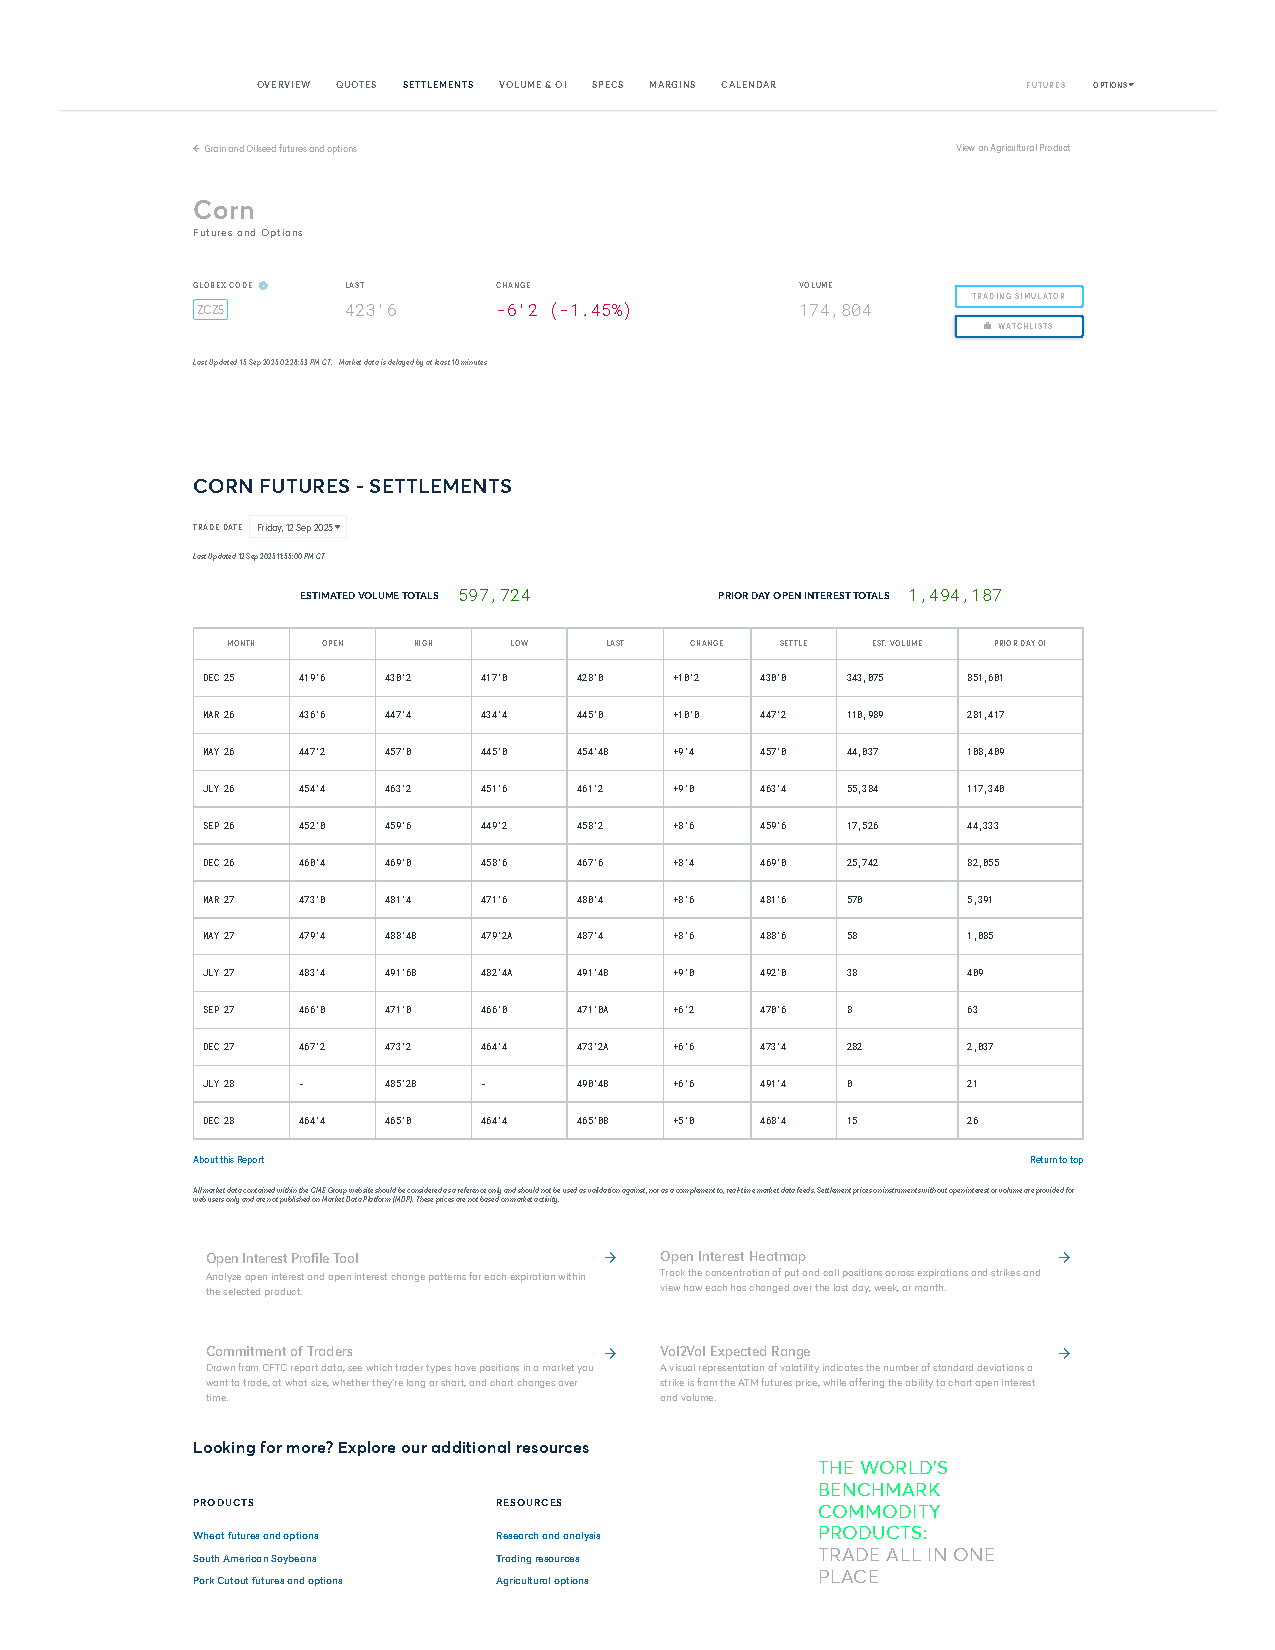
\includegraphics[width=0.99\textwidth]{appendix/CORN12SEP.pdf}
  \caption{Daily difference \(F-F^{*}\) and sign (backwardation vs.\ contango).}
  \label{fig:corn_settlements}
\end{figure}

\begin{figure}[h]
  \centering
  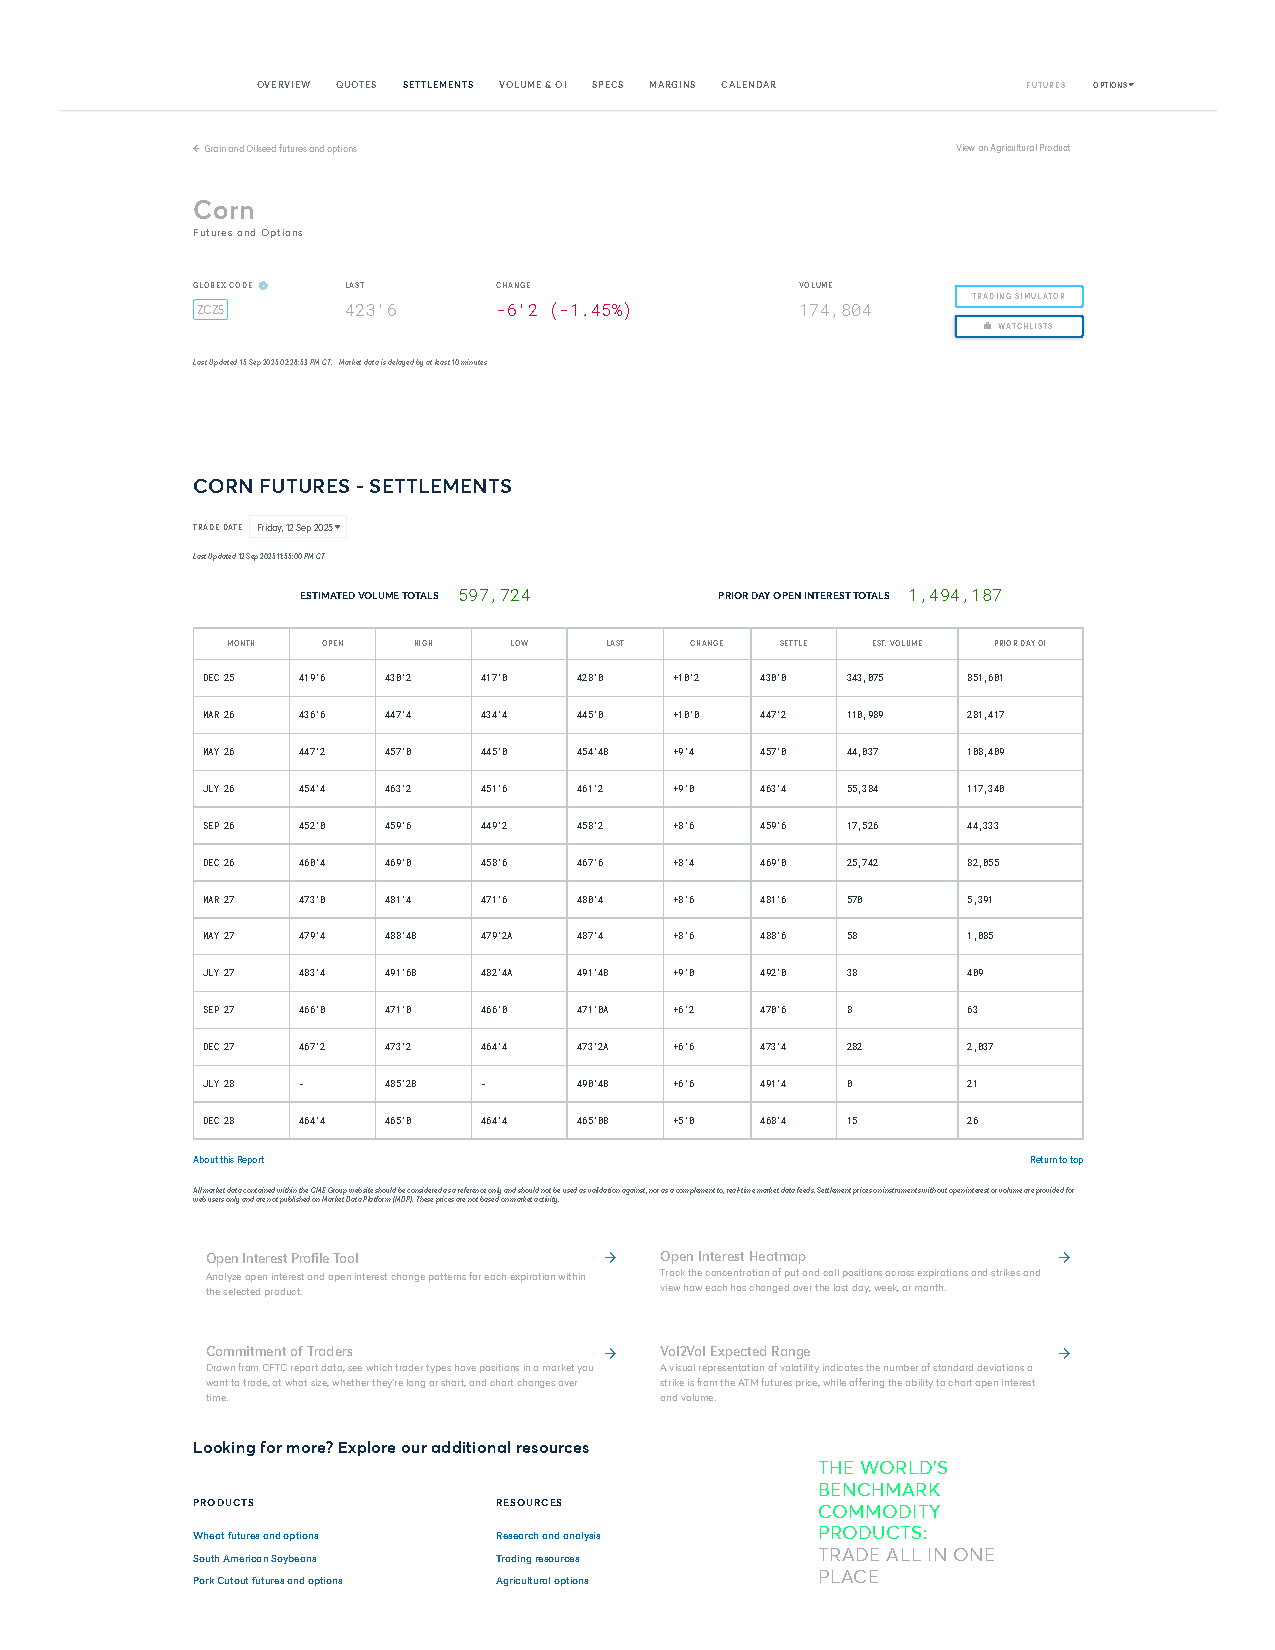
\includegraphics[width=0.99\textwidth]{appendix/CORN12SEP.pdf}
  \label{fig:corn_settlements}
\end{figure}

\begin{figure}[h]
  \centering
  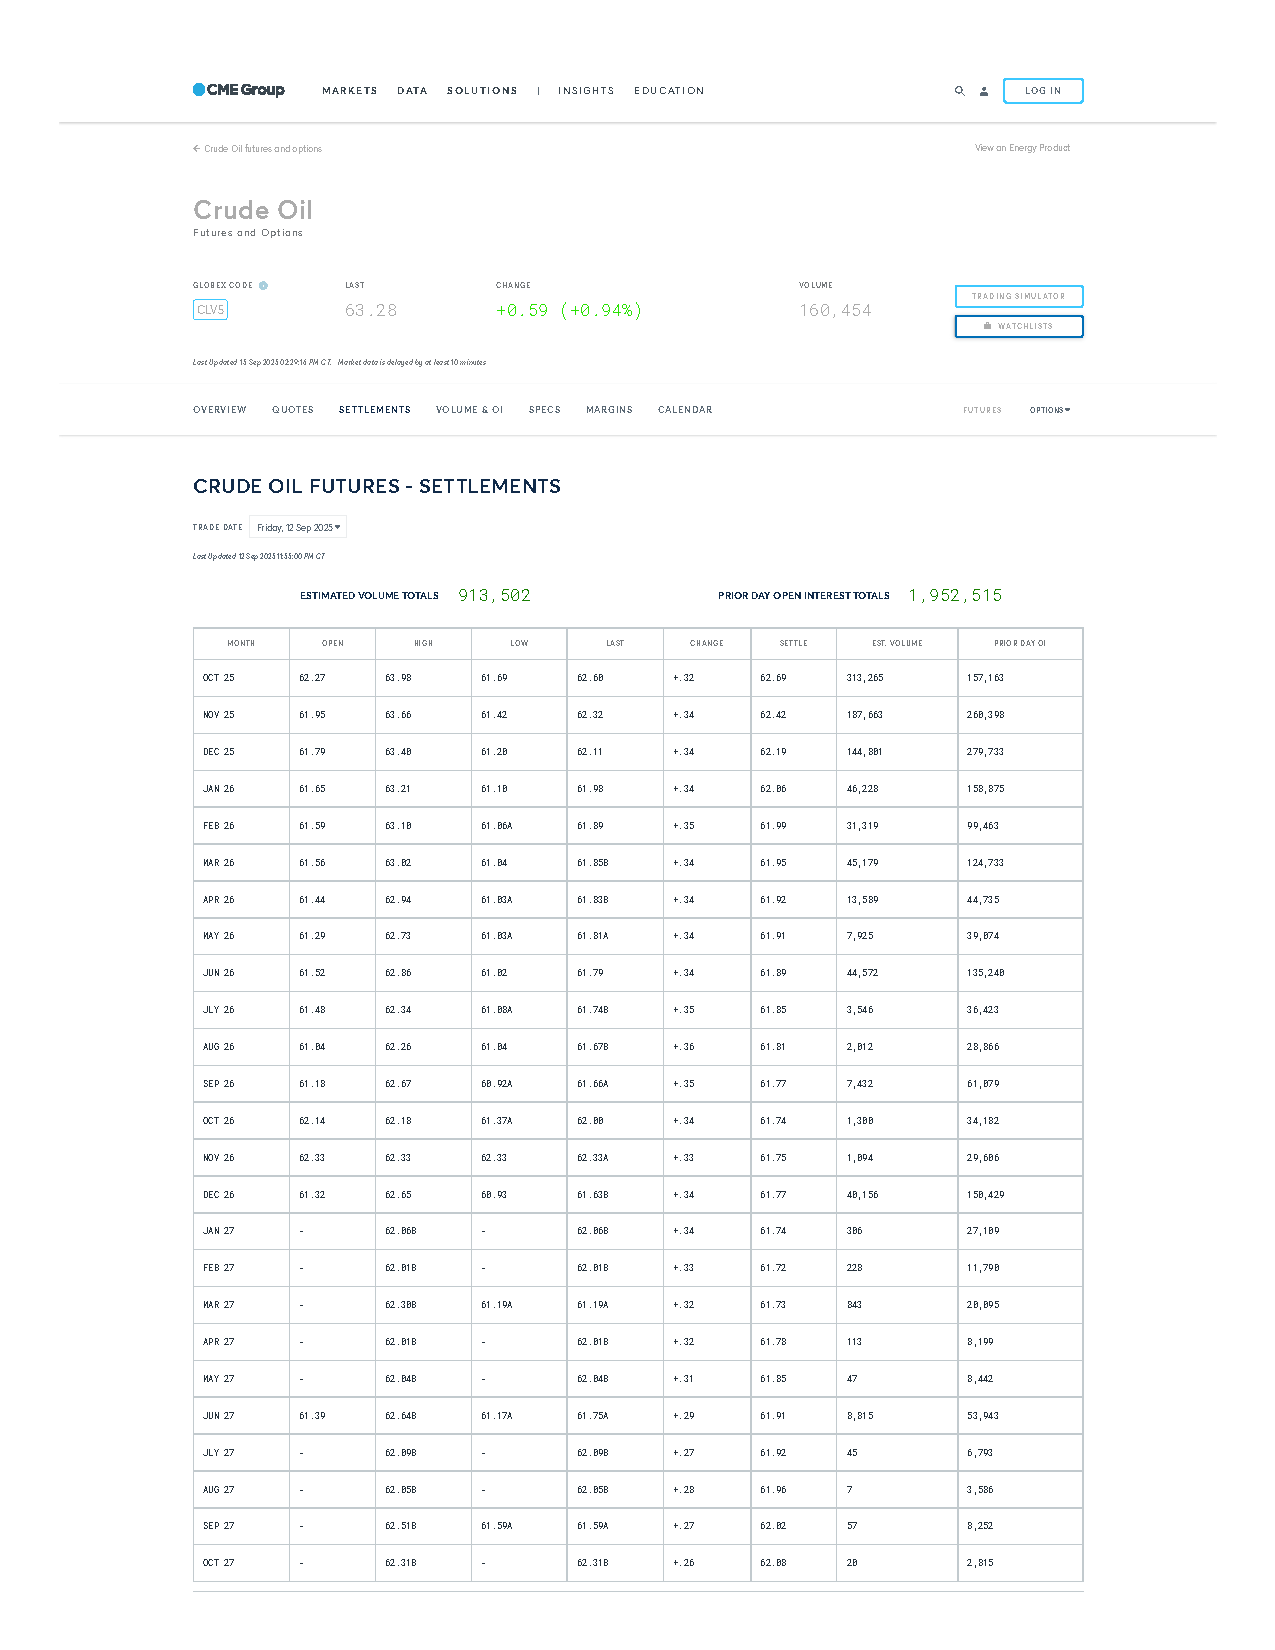
\includegraphics[width=0.99\textwidth]{appendix/CRUDEOIL12SEP.pdf}
  \label{fig:crudeoil_settlements}
\end{figure}

\begin{figure}[h]
  \centering
  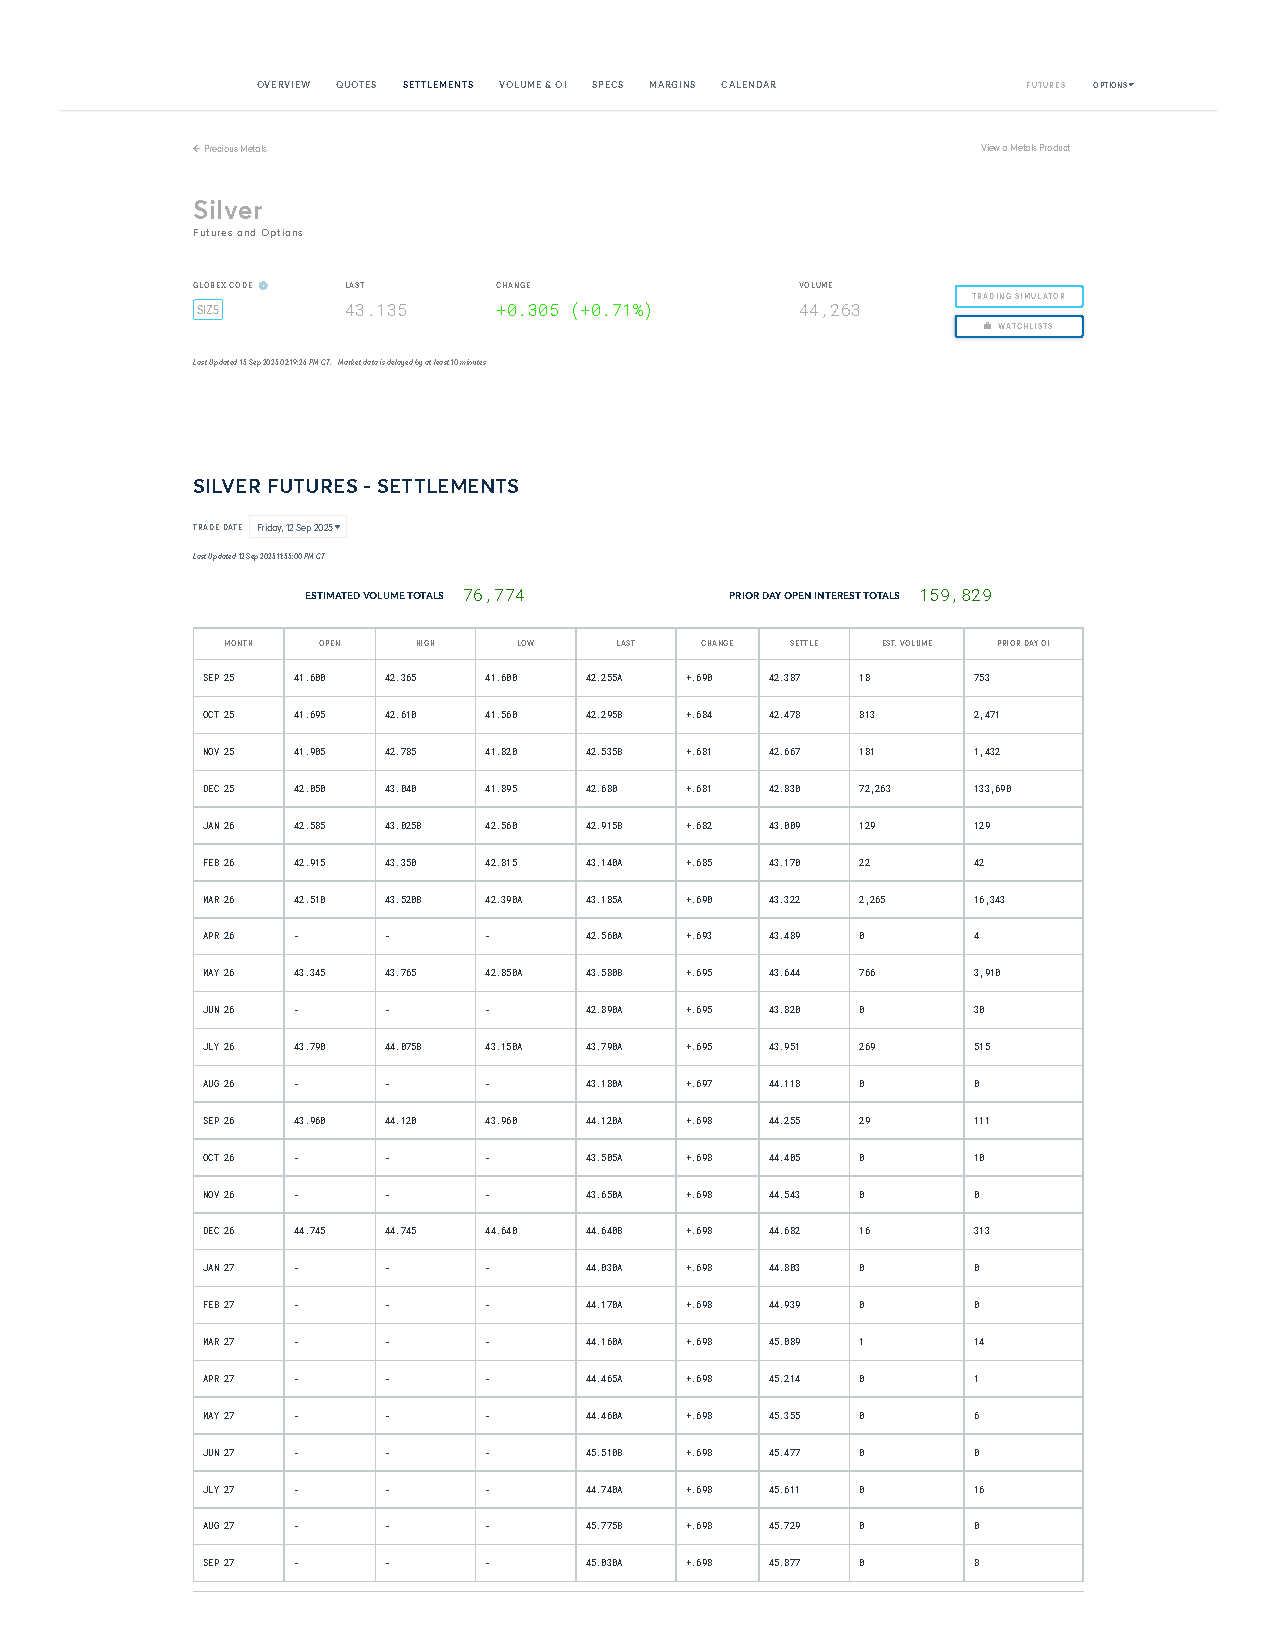
\includegraphics[width=0.99\textwidth]{appendix/SILVER12SEP.pdf}
  \label{fig:silver_settlements}
\end{figure}

\begin{figure}[h]
  \centering
  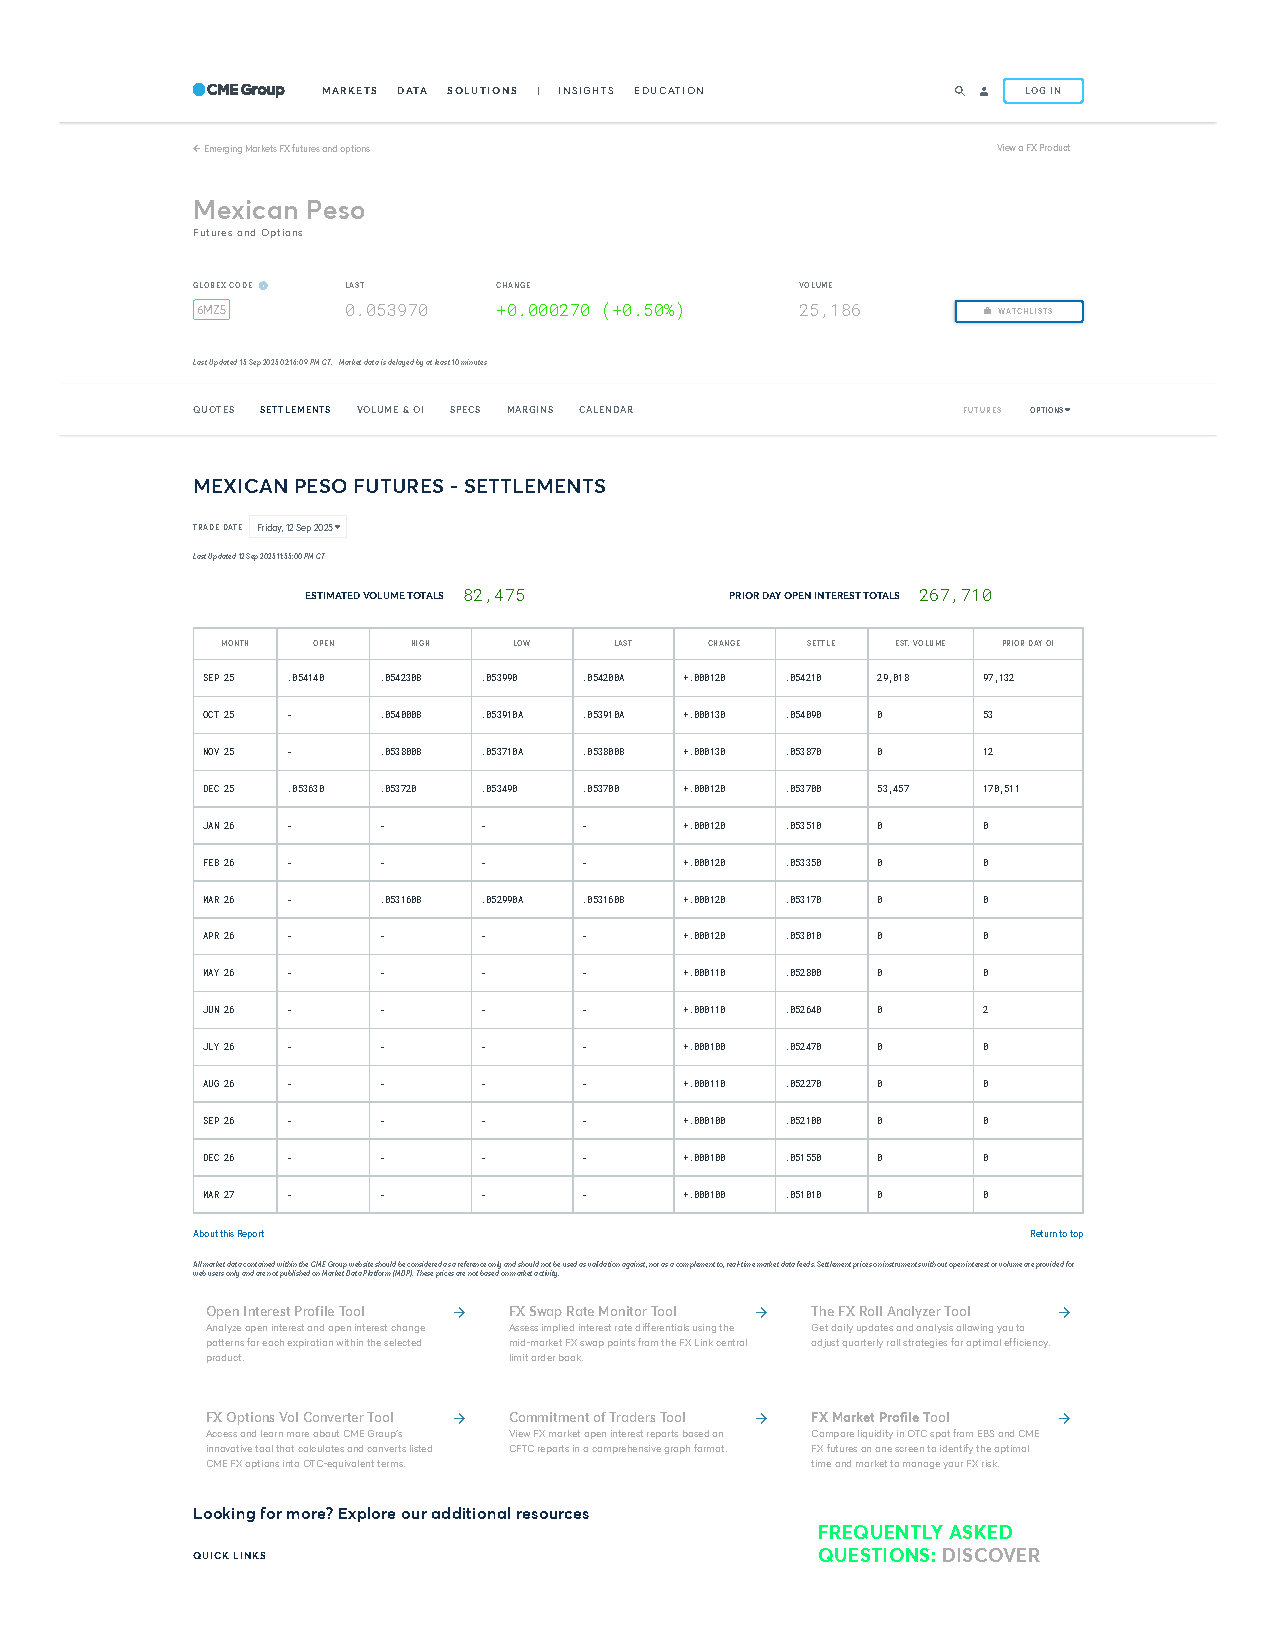
\includegraphics[width=0.99\textwidth]{appendix/MXNUSD12SEP.pdf}
  \label{fig:mxnusd_settlements}
\end{figure}

\begin{figure}[h]
  \centering
  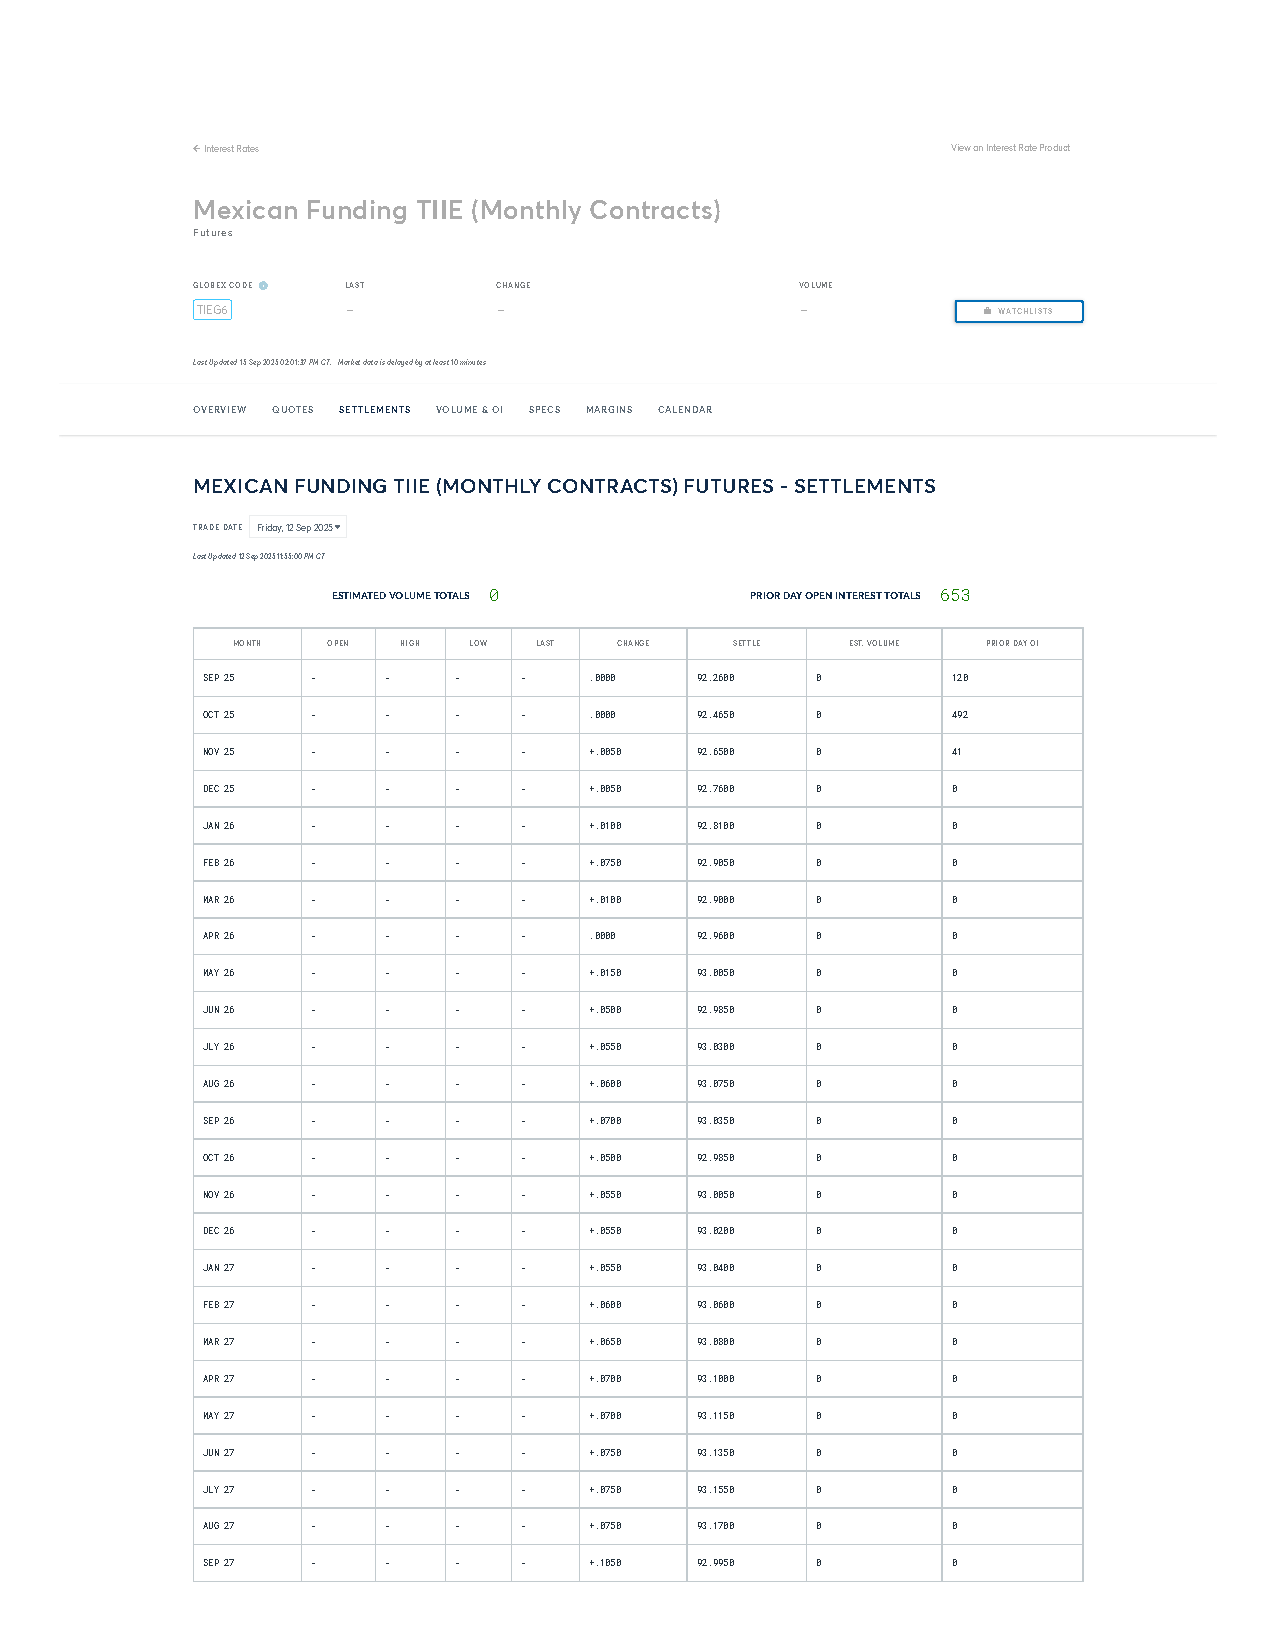
\includegraphics[width=0.99\textwidth]{appendix/TIIE12SEP.pdf}
  \label{fig:tiie_settlements}
\end{figure}

\begin{figure}[h]
  \centering
  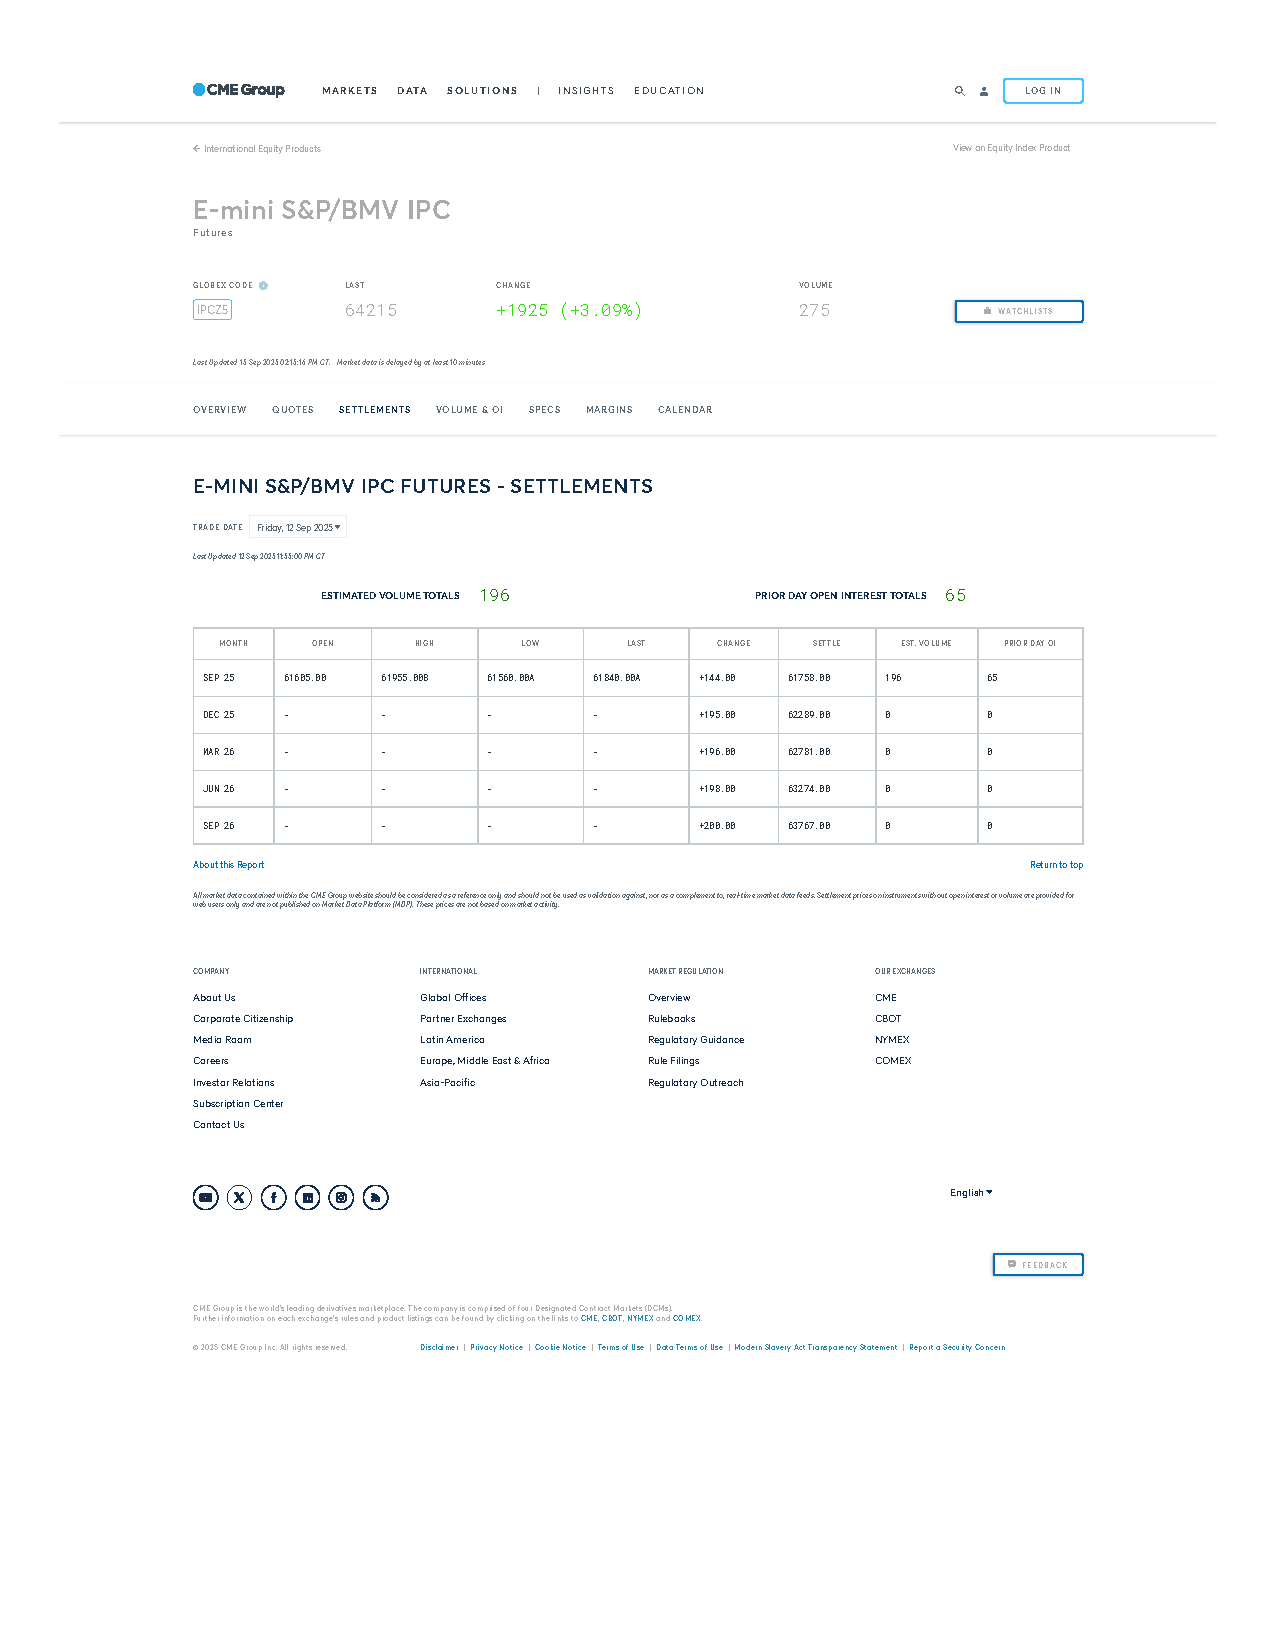
\includegraphics[width=0.99\textwidth]{appendix/IPC12SEP.pdf}
  \label{fig:ipc_settlements}
\end{figure}

\section{Appendix B: \\ Python Notebook }
\includepdf[pages=2-]{appendix/appendixB.pdf}

\end{document}